\documentclass[11pt]{book}
\usepackage{amsmath,mathtools}
\usepackage[utf8]{inputenc}
\usepackage[ngerman]{babel}
\usepackage{acronym}
\usepackage{graphicx} 
\usepackage{epstopdf}
\usepackage{svg}
\usepackage{multirow}
\usepackage{amssymb}
\usepackage{trfsigns}
\usepackage{setspace}
\usepackage{yfonts}

\onehalfspacing


%Hyperlinks package, links aus inhaltsverzeichnis
\usepackage{hyperref}
\hypersetup{
    colorlinks=false, %set true if you want colored links
    linktoc=all
}
%Blattformatierung
\usepackage{geometry}
\geometry{a4paper, top=25mm, left=30mm, right=20mm, bottom=20mm}

%Listing
\usepackage{courier}
\usepackage{listings}
\usepackage{color}
 \lstset{
   frame=tb,
   framexleftmargin=2.5em,
   basicstyle=\small\linespread{0.9}\bfseries\ttfamily,
   emph={square}, 
   emphstyle=\color{blue}\texttt,
   emph={[2]root,base},
   emphstyle={[2]\color{yac}\texttt},
   showstringspaces=false,
   flexiblecolumns=false,
   tabsize=2,
   numbers=left,
   numberstyle=\small\bfseries\ttfamily,
   numberblanklines=false,
   stepnumber=1,
   numbersep=10pt,
   xleftmargin=25pt
 }

\begin{document}
\tableofcontents
\def\presuper#1#2%
	{\mathop{}%
	\mathopen{\vphantom{#2}}^{#1}%
	\kern-\scriptspace%
	#2}
%Display vecotr in a reference frame
\newcommand{\vecBS}[4]{\presuper{#1}{\begin{pmatrix}
#2 \\ #3 \\ #4
\end{pmatrix}}}
%Boldsymbol shortcut
\newcommand{\bs}[1]{\boldsymbol{#1}}
%Bezugssystemdefinition
\newcommand{\defBS}[1]{\{#1\} [ \bs{e}_{{#1}_1},\bs{e}_{{#1}_2}, \bs{e}_{{#1}_3} ]}
%Projektionsmatrix
\newcommand{\pMat}[2]{\presuper{#1}{\bs{P}}^{#2}}
%Differenation in Respekt zu BS
\newcommand{\diffIn}[3]{\frac{\presuper{#1}{d{#2}}}{d#3}}
\newcommand{\partialDiffIn}[3]{\frac{\presuper{#1}{\partial{#2}}}{\partial #3}}
%Geschwindigkeit/Beschleunigung
\newcommand{\vel}[3]{\presuper{#1}{\bs{#2}}^{#3}}

%Rightarrow with spaceing
\newcommand{\rArrow}{\hspace{5pt}\rightarrow\hspace{5pt}}
%Inneres Produkt
\newcommand{\inProd}[2]{\langle {#1}, {#2} \rangle}

%System macro
\newcommand{\cSS}[3]{\textfrak{S}($\bs{#1}$,$\bs{#2}$,$\bs{#3}$)}
\newcommand{\dSS}[3]{\textfrak{D}($\bs{#1}$,$\bs{#2}$,$\bs{#3}$)}

%Laplace transform sign with spaces
\newcommand{\myLaplace}{\hspace{15pt}\laplace\hspace{15pt}}

\newcommand*{\signed}[1]{%
        \nolinebreak[3]\hspace*{\fill}\mbox{\emph{#1}}
    }

\ifx\FORMAT\undefined
\documentclass[11pt]{book}
\usepackage{amsmath,mathtools}
\usepackage[utf8]{inputenc}
\usepackage[ngerman]{babel}
\usepackage{acronym}
\usepackage{graphicx} 
\usepackage{epstopdf}
\usepackage{svg}
\usepackage{multirow}
\usepackage{amssymb}
\usepackage{trfsigns}
\usepackage{setspace}
\usepackage{yfonts}
%\usepackage{HsKatitle11}

\onehalfspacing


%Hyperlinks package, links aus inhaltsverzeichnis
\usepackage{hyperref}
\hypersetup{
    colorlinks=false, %set true if you want colored links
    linktoc=all,
    linkbordercolor = {white}
}
%Blattformatierung
\usepackage{geometry}
\geometry{a4paper, top=25mm, left=30mm, right=25mm, bottom=20mm}

%Listing
\usepackage{courier}
\usepackage{listings}
\usepackage{color}
 \lstset{
   frame=tb,
   framexleftmargin=2.5em,
   basicstyle=\small\linespread{0.9}\bfseries\ttfamily,
   emph={square}, 
   emphstyle=\color{blue}\texttt,
   emph={[2]root,base},
   emphstyle={[2]\color{yac}\texttt},
   showstringspaces=false,
   flexiblecolumns=false,
   tabsize=2,
   numbers=left,
   numberstyle=\small\bfseries\ttfamily,
   numberblanklines=false,
   stepnumber=1,
   numbersep=10pt,
   xleftmargin=25pt
 }
 
 \def\presuper#1#2%
	{\mathop{}%
	\mathopen{\vphantom{#2}}^{#1}%
	\kern-\scriptspace%
	#2}
%Display vecotr in a reference frame
\newcommand{\vecBS}[4]{\presuper{#1}{\begin{pmatrix}
#2 \\ #3 \\ #4
\end{pmatrix}}}
%Boldsymbol shortcut
\newcommand{\bs}[1]{\boldsymbol{#1}}
%Bezugssystemdefinition
\newcommand{\defBS}[1]{\{#1\} [ \bs{e}_{{#1}_1},\bs{e}_{{#1}_2}, \bs{e}_{{#1}_3} ]}
%Projektionsmatrix
\newcommand{\pMat}[2]{\presuper{#1}{\bs{P}}^{#2}}
%Differenation in Respekt zu BS
\newcommand{\diffIn}[3]{\frac{\presuper{#1}{d{#2}}}{d#3}}
\newcommand{\partialDiffIn}[3]{\frac{\presuper{#1}{\partial{#2}}}{\partial #3}}
%Geschwindigkeit/Beschleunigung
\newcommand{\vel}[3]{\presuper{#1}{\bs{#2}}^{#3}}

%Rightarrow with spaceing
\newcommand{\rArrow}{\hspace{5pt}\rightarrow\hspace{5pt}}
%Inneres Produkt
\newcommand{\inProd}[2]{\langle {#1}, {#2} \rangle}

%System macro
\newcommand{\cSS}[3]{\textfrak{S}($\bs{#1}$,$\bs{#2}$,$\bs{#3}$)}
\newcommand{\dSS}[3]{\textfrak{D}($\bs{#1}$,$\bs{#2}$,$\bs{#3}$)}

%Laplace transform sign with spaces
\newcommand{\myLaplace}{\hspace{15pt}\laplace\hspace{15pt}}

\newcommand*{\signed}[1]{%
        \nolinebreak[3]\hspace*{\fill}\mbox{\emph{#1}}
    }
\begin{document}
\fi

\chapter{Modellbildung Würfel auf Kante}
Dieses Kapitel widmet sich der Herleitung der Bewegungsgleichungen für den Fall, dass der Würfel auf einer seiner Kanten steht. Hierfür wird Kanes Methodik [Kane] angewandt, welche sich in die Untersuchung der kinematischen und kinetischen Gegebenheiten unterteilen lässt. Bei der Kinematikanalyse werden zunächst generalisierte Koordinaten eingeführt um die Konfiguration des Systems zu beschreiben. Des weiteren werden Bezugssysteme verwendet um einzelnen Körper des Gesamtsystems im dem mathematischen Modell darzustellen. Die kinematische Untersuchung endet mit der Definition der generalisierten Geschwindigkeiten und Bestimmung der partiellen Geschwindigkeiten, welche als Betrag und Richtung der Systembewegung interpretiert werden können.
In dem zweiten Teil des Kapitels wird die Kinematik betrachtet. Zu Beginn werden die resultierenden Drehmomente formuliert, welche auf die verschiedenen Körper wirken. Diese werden verwendet um mit Hilfe der partiellen Geschwindigkeiten die generalisierten aktiven Kräfte $F_i$ zu ermitteln. Analog werden die Trägheitsmomente und daraus die generalisierten Trägheitskräfte $F^*_i$ berechnet, welche mittels Kanes Gleichung $F_i+F^*_i=0$ auf die gesuchten Bewegungsgleichungen führen. Zuletzt wird die Auswirkung der generalisierten Geschwindigkeiten auf die resultierenden Bewegungsgleichungen an Hand eines einfachen Beispiels diskutiert.
\newpage
\section{Untersuchung der Kinematik}
Der erste Schritt besteht darin die kinematischen Zusammenhänge des Systems zu analysieren. Im Fall, dass der Würfel auf einer Kante balanciert, verfügt dieser über zwei rotatorische Freiheitsgrade. Der erste wird von der generalisierten Koordinate $\varphi$ beschrieben und gibt die Orientierung des Würfelgehäuses wieder. Die zweite generalisierte Koordinate $\psi$ erfasst die Rotation der Schwungmasse relativ zu dem Würfelgehäuse.
\begin{figure}[!ht]
\centering
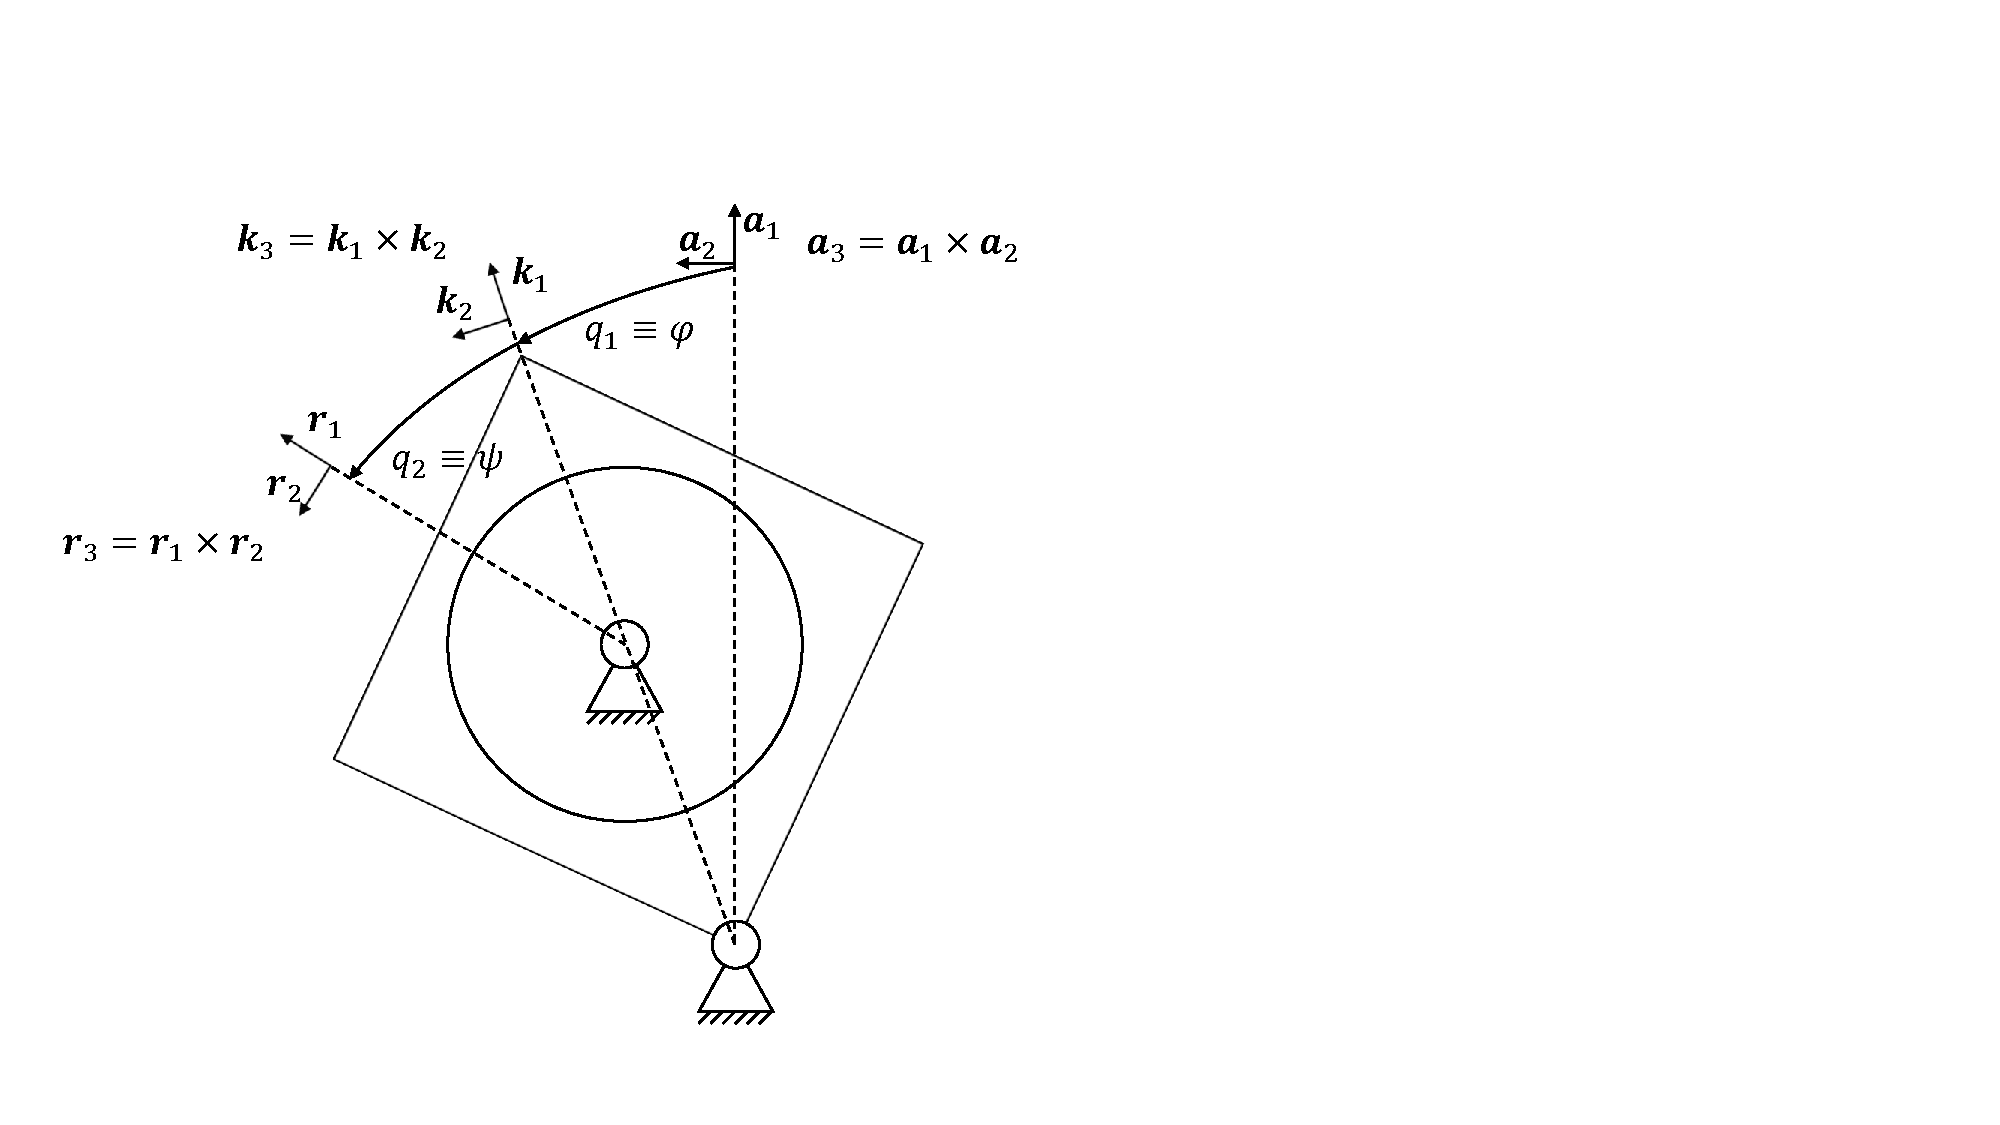
\includegraphics[width=0.6\linewidth, trim={1cm 1.5cm 18cm 3.5cm}, clip]{img/ModellWuerfelseite}
\caption{Kinematikplan des Würfels auf einer Kante, Quelle: eigene Darstellung}
\label{skizze_dynamik_edge}
\end{figure}

Um die Körper des Systems zu modellieren werden im nächsten Schritt die Bezugssysteme $A$, $K$ und $R$ eingeführt, wobei ein beliebiges Bezugssystem $B$ durch drei Vektoren $\bs{b_i} \ i \in \{1,2,3\}$ definiert wird. Die Vektoren $\bs{b_i}$ werden als Vektorbasis bezeichnet.\footnote{Allgemein genügen drei linear unabhängige Vektoren als Vektorbasis, allerdings werden in dieser Arbeit ausschließlich paarweise orthogonale Einheitsvektoren verwendet, da diese eine einfachere Handhabung ermöglichen. Im weiteren Verlauf wird nicht explizit erwähnt, dass es sich bei den Vektorbasen um paarweise orthogonale Einheitsvektoren handelt.} In diesem Fall ist $A$ ein Intertialsystem, das heißt die Ausrichtung der Vektoren $\bs{a_i}$ ist konstant. Deshalb wird $A$ bzw. dessen Vektorbasis auch als raumfest bezeichnet. Bei $K$ handelt es sich um ein körperfestes Bezugssystem, die Vektoren $\bs{k_i}$ sind an dem Würfelgehäuse fixiert und ändern ihre Ausrichtung in Abhängigkeit von $\varphi$. Das Bezugssystem $R$ ist ebenfalls körperfest, wobei die Vektorbasis an der Schwungmasse fixiert ist. Foglich beschreiben die Koordiaten $\varphi$ und $\psi$ die Rotation von $K$ relativ zu $A$ bzw. von $R$ gegenüber $K$. 

Mittels eines Bezugssystems kann ein bliebiger Vektor als Linearkombination der Vektorbasis dargestellt werden. Als Beispiel sei der Ortsvektor $\bs{c}$ des Würfelschwerpunktes geannt, wobei das verwendete Bezugssystem durch den vorangehenden Superskript gekennzeichnet wird.
\begin{equation}
\bs{c} = l\idx{C} \cdot \bs{k}\idx{1} + 0 \cdot \bs{k}\idx{2} + 0 \cdot \bs{k}\idx{3} = \vecBS{K}{l\idx{C}}{0}{0}
\end{equation}
Um nun die Komponenten $\alpha_i$ des Vektors $\bs{c}$ in dem Bezugssystem $A$ zu erhalten, muss das Skalarprodukt $\inProd{\bs{a}_i}{\bs{c}}$ berechnet werden. Wird dieser Ansatz auf alle drei Komponenten appliziert ergibt sich der Zusammenhang\footnote{Um die allgemeine Gültigkeit der linearen Abbildung zu verdeutlichen wird in dieser Gleichung die Definition $\bs{c}=\vecBS{K}{l_C}{0}{0}\equiv\vecBS{K}{\beta_1}{\beta_2}{\beta_3}$ verwendet.}
\begin{equation}
\begin{split}
\bs{c} &= \vecBS{A}{\alpha\idx{1}}{\alpha\idx{2}}{\alpha\idx{3}} = \inProd{\bs{c}}{\bs{a}\idx{1}}\cdot \bs{a}\idx{1} + \inProd{\bs{c}}{\bs{a}\idx{2}}\cdot\bs{a}\idx{2} + \inProd{\bs{c}}{\bs{a}\idx{3}}\cdot\bs{a}\idx{3} 
= \vecBS{A}{\inProd{\bs{c}}{\bs{a}\idx{1}}}{\inProd{\bs{c}}{\bs{a}\idx{2}}}{\inProd{\bs{c}}{\bs{a}\idx{3}}}
\\
&= \vecBS{A}
{\beta\idx{1}\cdot\inProd{\bs{a}\idx{1}}{\bs{k}\idx{1}} + \beta\idx{2}\cdot\inProd{\bs{a}\idx{1}}{\bs{k}\idx{2}} + \beta\idx{3}\cdot\inProd{\bs{a}\idx{1}}{\bs{k}\idx{3}}}
{\beta\idx{1}\cdot\inProd{\bs{a}\idx{2}}{\bs{k}\idx{1}} + \beta\idx{2}\cdot\inProd{\bs{a}\idx{2}}{\bs{k}\idx{2}} + \beta\idx{3}\cdot\inProd{\bs{a}\idx{2}}{\bs{k}\idx{3}}}
{\beta\idx{1}\cdot\inProd{\bs{a}\idx{3}}{\bs{k}\idx{1}} + \beta\idx{2}\cdot\inProd{\bs{a}\idx{3}}{\bs{k}\idx{2}} + \beta\idx{3}\cdot\inProd{\bs{a}\idx{3}}{\bs{k}\idx{3}}}
\\
&= \presuper{K}{\begin{pmatrix}
\underbrace{
\begin{bmatrix}
\inProd{\bs{a}\idx{1}}{\bs{k}\idx{1}} & \inProd{\bs{a}\idx{1}}{\bs{k}\idx{2}} & \inProd{\bs{a}\idx{1}}{\bs{k}\idx{3}} \\
\inProd{\bs{a}\idx{2}}{\bs{k}\idx{1}} & \inProd{\bs{a}\idx{2}}{\bs{k}\idx{2}} & \inProd{\bs{a}\idx{2}}{\bs{k}\idx{3}} \\
\inProd{\bs{a}\idx{3}}{\bs{k}\idx{1}} & \inProd{\bs{a}\idx{3}}{\bs{k}\idx{2}} & \inProd{\bs{a}\idx{3}}{\bs{k}\idx{3}}
\end{bmatrix}}_{\equiv \pMat{K}{A}} \cdot \underbrace{\begin{bmatrix}
\beta\idx{1} \\ \beta\idx{2} \\ \beta\idx{3}
\end{bmatrix}}_{= \presuper{K}{\bs{c}}}
\end{pmatrix}} 
= \presuper{A}{\begin{pmatrix}
\begin{bmatrix}c_{\varphi} & -s_{\varphi} & 0 \\ s_{\varphi} & c_{\varphi} & 0 \\ 0 & 0 & 1 \end{bmatrix} \cdot \presuper{K}{\bs{c}} \end{pmatrix}}\,.
\end{split}
\end{equation}
Somit handelt es sich bei der Projektion eines Vektors, welcher in einem beliebigen Bezugssystem $A$ dargestellt ist, in ein weiteres Bezugssystem $B$ um eine lineare Abbildung. Die Abbildungsvorschrift wird durch die Matrix $\pMat{B}{B}$ definiert. Des weiteren zeigt dieses Beispiel die perspektivische Bedeutung eines Bezugssystem. Wird der Vektor $\bs{c}$ in $K$ dargestellt hängt er lediglich von der Länge $l_C$ ab und ist folglich konstant. Aus der Perspektive von $A$ ist der Vektor eine Funktion von $\varphi$ und somit variabel. Die Begründung hierfür ist, dass das Intertialsystem $A$ die Bewegung des Würfels im Raum wahrnimmt, wodurch der Ortsvektor des Schwerpunktes variable erscheint.
Im Gegensatz dazu erfasst das köperfeste Bezugssystem $K$ einen Vektor aus der Perspektive des Würfelkörpers. Aus diesem Grund ist der in $K$ dargstellte Ortsvektor $\presuper{K}{\bs{c}}$ des Schwerpunktes konstant.
Dieser Umstand kann genutzt werden, indem ein Vektor zunächst in einer einfachen Form dargestellt und anschließend in das gewünschte Bezugssystem projiziert wird. Als Beispiel dient die Berechnung des Gravitationsmoments $\bs{T}^{K/O}$. Der Erdbeschleunigungsvektor $\bs{g}$ ist im Inertialsystem $A$ konstant und wird von dort in das körperfeste System $K$ transformiert.
\begin{equation}
\begin{split}
\bs{T}^{K/O} = \bs{c}\times m\cdot\bs{g} &= \vecBS{K}{l\idx{C}}{0}{0}\times \vecBS{A}{-m\cdot g}{0}{0} = \vecBS{K}{l\idx{C}}{0}{0}\times\presuper{K}{\begin{pmatrix}
\pMat{A}{K}\cdot \vecBS{A}{-m\cdot g}{0}{0}
\end{pmatrix}}
\\
&= \vecBS{K}{l\idx{C}}{0}{0}\times \vecBS{K}{-c_{\varphi}\cdot m\cdot g}{s_{\varphi}\cdot m\cdot g}{0} = \vecBS{K}{0}{0}{s_{\varphi}\cdot m\cdot g\cdot l\idx{C}}
\end{split}
\end{equation}
Dieses Beispiel zeigt, dass die Einführung von Bezugssystemen eine eindeutige Notation und Vorgehensweise zur Berechnung von vektorwertigen Funktionen mit sich bringt. Man möge bei diesem Anwendungsfall argumentieren, dass die trigonometrischen Zusammenhänge des Gravitationsmomentes auch aus der Abbildung \ref{skizze_dynamik_edge} ablesen lassen. Allerdings ist die hier betrachtete Vorgehensweise allgemeingültig und kann auf beliebig komplexe Systeme angewendet werden. Beispielsweise kann das Gravitationsmoment in dem Fall, dass der Würfel auf einer Ecke steht, kaum mehr aus einer Skizze bestimmt werden.

Zur vollständigen Beschreibung der Kinematik müssen die Geschwindigkeiten des Systems ermittelt werden, welche aus den Ableitungen der Winkel $\varphi$ und $\psi$ hervorgehen. Als Beispiel für die Ableitung eines Vektors dient wieder der Ortsvektor $\bs{c}$ des Schwerpunktes. Dieser ist aus der Perspektive des Bezugssystem $K$ konstant, folglich verschwindet auch dessen Ableitung bzw. Geschwindigkeit. Wird der Vektor aber in $A$ abgebildet hängt dieser von der Zeitfunktion $\varphi(t)$ ab. Deshalb muss bei der Ableitung eines Vektors das Bezugssystem angegeben werden, aus dessen Perspektive differenziert wird ([Kane], S.25ff). Wenn $\bs{c}$ in $A$ differenziert werden soll, so muss dieser zunächst in $A$ dargestellt und anschließend komponentenweise nach der Zeit abgeleitet werden.
\begin{equation}
\frac{\presuper{A}{d}\bs{c}}{dt} = \frac{d(c_{\varphi}\cdot l\idx{C})}{dt}\cdot \bs{a}\idx{1} + \frac{d(s_{\varphi}\cdot l\idx{C})}{dt}\cdot \bs{a}\idx{2} + \frac{d(0)}{dt}\cdot \bs{a}\idx{3} = \vecBS{A}{-s_{\varphi}\cdot \dot{\varphi}\cdot l\idx{C}}{c_{\varphi}\cdot \dot{\varphi}\cdot l\idx{C}}{0}
\end{equation}
Hieraus folgt, dass auch die Geschwindigkeiten eines Körpers lediglich als relativ zu einem Bezugssystem angegeben werden können. Somit beschreibt $\vel{B}{v}{P}$ die Geschwindigkeit bzw. $\vel{B}{a}{P}$ die Beschleunigung  eines Punktes oder Körpers $P$  relativ zu einem Bezugssystem $B$. Diese werden wie folgt definiert ([Kane], S.28).
\begin{equation}
\vel{B}{v}{P} = \frac{\presuper{B}{d\bs{p}}}{dt} \hspace{35pt} \vel{B}{a}{P} = \frac{\presuper{B}{d}\vel{B}{v}{P}}{dt}
\end{equation}
Die selbe Notation wird für Winkelgeschwindigkeiten und -beschleunigungen eingeführt, wobei $\vel{A}{\omega}{B}$ die Winkelgeschwindigkeit und $\vel{A}{\alpha}{B}$ die Winkelbeschleunigung eines Punktes oder Bezugssystems $B$ relativ zu $A$ ist. Die Geschwindigkeit relativ zu einem Inertialsystem wird auch als absolute Geschwindigkeit bezeichnet. Für die Bezugssysteme $K$ und $R$ lassen sich mit Hilfe der Abbildung \ref{skizze_dynamik_edge} die folgenden Winkelgeschwindigkeiten bestimmen, wobei die absolute Winkelgeschwindigkeit eines Bezugssystems die Summe seiner relativen Winkelgeschwindigkeiten ist ([Kane], S.24f).
\begin{equation}
\vel{A}{\omega}{K} = \vecBS{K}{0}{0}{\dot{\varphi}} \hspace{15pt} \vel{K}{\omega}{R} = \vecBS{R}{0}{0}{\dot{\psi}} \hspace{15pt} \vel{A}{\omega}{R} = \vel{A}{\omega}{K} + \vel{K}{\omega}{R} = \vecBS{A}{0}{0}{\dot{\varphi} + \dot{\psi}}
\end{equation}
Der letzte Schritt bei der Untersuchung der Kinematik besteht darin die  generalisierten Geschwindigkeiten zu definieren und daraus die partiellen Geschwindigkeiten zu berechnen. Bei den generalisierten Geschwindigkeiten $u_i$ handelt es sich um skalare Größen deren Anzahl gleich der Zahl der generalisierten Koordinaten ist. Die generalsierten Geschwindigkeiten sind für gewöhnlich abhängig von den Zeitableitungen der generalisierten Geschwindigkeiten $\dot{q}_i$, wobei sie so gewählt werden müssen, dass die Definitionen eindeutig nach den Ableitungen $\dot{q}_i$ aufgelöst werden können. Die Einführung der generalisierten Geschwindigkeiten verfolgt das Ziel, möglichst einfache Ausdrücke für die absoluten Geschwindigkeiten $\vel{A}{\omega}{K}$ und $\vel{A}{\omega}{R}$ und, wie sich im späteren Verlauf zeigen wird, einfachere Ausdrücke der Bewegungsgleichungen zu erhalten. Deshalb werden hier die  Definitionen 
\begin{equation}
\begin{split}
u\idx{1} = u\idx{K} \equiv \dot{\varphi} &\hspace{35pt} u\idx{2} = u\idx{R} \equiv \dot{\varphi} + \dot{\psi} \\
\vel{A}{\omega}{K} = \vecBS{K}{0}{0}{u\idx{1}} & \hspace{35pt} \vel{A}{\omega}{R}=\vecBS{K}{0}{0}{u\idx{2}}
\end{split}
\end{equation}
gewählt. Diese Geschwindigkeitsausdrücke können auch in die Form
\begin{equation}
\vel{A}{\omega}{K} = u\idx{1}\cdot \vel{A}{\omega}{K}\idx{1} + u\idx{2} \cdot \vel{A}{\omega}{K}\idx{2} \hspace{35pt} \vert \hspace{15pt} \vel{A}{\omega}{K}\idx{1} = \bs{k}\idx{3}, \hspace{10pt} \vel{A}{\omega}{K}\idx{2} = \bs{0}
\end{equation}
\begin{equation}
\vel{A}{\omega}{R} = u\idx{1}\cdot \vel{A}{\omega}{R}\idx{1} + u\idx{2} \cdot \vel{A}{\omega}{R}\idx{2} \hspace{35pt} \vert \hspace{15pt} \vel{A}{\omega}{R}\idx{1} = \bs{0}, \hspace{10pt} \vel{A}{\omega}{R}\idx{2} = \bs{k}\idx{3}
\end{equation}
gebracht werden, wobei die Größen $\vel{A}{\omega}{K}_i$ und $\vel{A}{\omega}{R}_i$ partielle Geschwindigkeiten genannt werden. Diese Zerlegung kann so interpretiert werden, dass die generalisierten Geschwindigkeiten $u_i$ als skalare Größen den Betrag der Bewegung und die entsprechende partielle Geschwindigkeit, als vektorielle Größe, deren Richtung wiedergibt. Die Vorteile diese Zerlegung in generalisierte und partielle Geschwindigkeiten wird sich im folgenden Abschnitt zeigen.

\newpage
\section{Untersuchung der Kinetik}
Im nächsten Schritt wird die Kinematik des Systems untersucht, um die Bewegungsgleichungen herzuleiten. Hierfür werden zunächst die Drehmomente analysiert, welche auf den Würfelgehäuse und die Schwungmasse wirken. Letztere wird einerseits von dem Motormoment $\bs{T}^{R/M}_M$ beschleunigt, andererseits wirkt ein verzögerndes Reibmoment $\bs{T}^{R/M}_M$. Das Reibmoment wird als proportional zu der Winkelgeschwindigkeit $\dot{\psi}$ modelliert.
\begin{equation}
\bs{T}^{R/M} = \bs{T}^{R/M}_M + \bs{T}^{R/M}_R = [T_M - C_{\psi}(u_2 - u_1)]\cdot \bs{k}_3
\end{equation}
Das Motor- und Reibmoment wirken an dem Verbindungspunkt zwischen Schwungmasse und Würfelgehäuse. Deshalb beeinflussen die beiden den Würfelkörper in umgekehrter Richtung. Des weiteren wird das Würfelgehäuse von dem Gravitationsmoment $\bs{T}^{K/O}_G$ beschleunigt. Die Summe der Komponenten ergibt das resultierende Drehmoment $\bs{T}^{K/O}$.
\begin{equation}
\bs{T}^{K/O} = T^{K/O}_G - \bs{T}^{R/M}_M - \bs{t}^{R/M}_R = [m\cdot g\cdot l_C\cdot s_{\varphi} - T_M + C_{\psi}(u_2 - u_1)] \cdot \bs{k}_3
\end{equation}
Um die Bewegungsgleichungen zu ermitteln, werden die generalisierten aktiven Kräfte $F_i$ benötigt. Hierfür werden die Skalarprodukte der Drehmomente, welche auf die Körper wirken, und die partiellen Winkelgeschwindigkeiten, des entsprechenden Körpers, berechnet. Die Summe über alle Körper ergibt die generalisierte aktive Kraft $F_i$.
\begin{equation}
\begin{split}
F_1 &= \inProd{\bs{T}^{K/O}}{\vel{A}{\omega}{K}_1} + \inProd{\bs{T}^{R/M}}{\vel{A}{\omega}{R}_1}
 = m\cdot g\cdot l_C\cdot s_{\varphi} - T_M + C_{\psi}(u_2 - u_1)
\\
F_2 &= \inProd{\bs{T}^{K/O}}{\vel{A}{\omega}{K}_2} + \inProd{\bs{T}^{R/M}}{\vel{A}{\omega}{R}_2} = T_M - C_{\psi}(u_2 - u_1)
\end{split}
\end{equation}
Die partiellen Geschwindigkeiten können als Bewegungsrichtungen der Körper interpretiert werden. Somit stellen die generalisierten Kräfte $F_i$ den Beitrag der Drehmomente in die jeweilige Bewegungsrichtung wieder.

Als Gegenstück zu den generalisierten aktiven Kräften müssen nun die generalisierten Trägheitskräfte $F^*_i$ ermittelt werden. Das resultierende Trägheitsmoment der Schwungmasse ergibt sich aus dem Produkt des Skalars $I_R$, welcher das Massenträgheitsmoment des Körpers relativ zu $M$ beschreibt, und der Winkelbeschleunigung $\vel{A}{\alpha}{R}$.\footnote{Die hier verwendete Berechnung ist nicht allgemeingültig. Für gewöhnlich wird zur Berechnung der Trägheitsmomente ein Trägheitstensor $\bs{I}$ verwendet. Die in einem späteren Kapitel erläutert.}
\begin{equation}
\bs{T}^{R/M}_* = -I_R\cdot \vecBS{K}{0}{0}{\dot{u}_2}
\end{equation}
Das Trägheitsmoment des Würfelkörpers berechnet sich aus dessen Trägheitsskalar $I_K$ und der Winkelbeschleunigung $\vel{A}{\alpha}{K}$. Die Größe $I_K$ ist die Summe des Massenträgheitsmoments des Würfelgehäuses $I^{GH/O}$ und dem Einfluss der Schwungmasse, wleche dabei als Punkt mit der Masse $m_R$ und dem Abstand $l_{MO}$ betrachtet wird.
\begin{equation}
\bs{T}^{K/O}_* = -(I^{GH/O} + m_R\cdot l^2_{MO})\cdot \vecBS{K}{0}{0}{\dot{u}_1} = -I_K\cdot \vecBS{K}{0}{0}{\dot{u}_1}
\end{equation}
Die generalisierten Trägheitskräfte $F^*_i$ werden wieder aus der folgenden Summe von Skalarprodukten berechnet.
\begin{equation}
\begin{split}
F^*_1 &= \inProd{\bs{T}^{K/O}_*}{\vel{A}{\omega}{K}_1} + \inProd{\bs{T}^{R/M}_*}{\vel{A}{\omega}{R}_1} = -I_K\cdot \dot{u}_1 
\\
F^*_2 &= \inProd{\bs{T}^{K/O}_*}{\vel{A}{\omega}{K}_2} + \inProd{\bs{T}^{R/M}_*}{\vel{A}{\omega}{R}_2} = -I_R\cdot \dot{u}_2 
\end{split}
\end{equation}
Die Bewegunsgleichungen resultieren nun aus Kanes Gleichung $F_i + F^*_i = 0$.
\begin{equation}
\begin{split}
F_1 + F^*_1 = 0 &\hspace{15pt}\leftrightarrow\hspace{15pt} I_K\cdot \dot{u}_1 = m\cdot g\cdot l_C\cdot s_{\varphi} - T_M + C_{\psi}(u_2 - u_2) 
\\
F_2 + F^*_2 = 0 &\hspace{15pt}\leftrightarrow\hspace{15pt} I_R\cdot \dot{u}_2 = T_M - C_{\psi}(u_2 - u_1)
\end{split}
\end{equation}


Rückblickend kann Kanes Methodik in die folgenden Schritte unterteilt werden. Zunächst wird die Kinematik des Systems analysiert, wobei die Körper mit Hilfe von Bezugssystemen modelliert werden. Die Definition von generalisierten Geschwindigkeiten ermöglicht die Bestimmung der partiellen Geschwindigkeiten, wodurch die Bewegung des Systems in eine Art Betrag und Richtung unterteilt wird. Anschließend werden die partiellen Geschwindigkeiten genutzt um die wirkenden Kräfte und Trägheitskräfte in die Bewegungsrichtungen zu projizieren. Hieraus resultieren die generalisierten aktiven Kräfte und generalisierten Trägheitskräfte, welche mittels Kanes Gleichung auf die gesuchten Bewegungsgleichungen führen.

Um die Bedeutung der generalisierten Geschwindigkeiten zu verdeutlichen wird der Fall betrachtet, dass die folgende Definition gewählt wird.
\begin{equation}
\tilde{u}_1 \equiv \dot{\varphi} \hspace{35pt} \tilde{u}_2 \equiv \dot{\psi}
\end{equation}
\begin{equation}
\begin{split}
\vel{A}{\tilde{\omega}}{K}_1 = \bs{k}_3 &\hspace{35pt} \vel{A}{\tilde{\omega}}{K}_2 = 0
\\
\vel{A}{\tilde{\omega}}{R}_1 = 0 &\hspace{35pt} \vel{A}{\tilde{\omega}}{R}_2 = \bs{k}_3
\end{split}
\end{equation}
\begin{equation}
\begin{split}
\tilde{F}_1 = m\cdot g\cdot l_C\cdot s_{\varphi} &\hspace{35pt} \tilde{F}_2 = T_M - C_{\psi}(u_2-u_1) 
\\
\tilde{F}^*_1 = -I_R\cdot (\dot{\tilde{u}}_1 + \dot{\tilde{u}}_2) - I_K\cdot \dot{\tilde{u}}_1 &\hspace{35pt} \tilde{F}^*_2 = -I_R\cdot (\dot{\tilde{u}}_1 + \dot{\tilde{u}}_2)
\end{split}
\end{equation}
\begin{equation}
\begin{split}
\tilde{F}_1 + \tilde{F}^*_1 = 0 &\hspace{15pt}\leftrightarrow\hspace{15pt} I_k\cdot \dot{\tilde{u}}_1 + I_R\cdot (\dot{\tilde{u}}_1+\dot{\tilde{u}}_2) = m\cdot g\cdot l_C\cdot s_{\varphi} 
\\
\tilde{F}_2 + \tilde{F}^*_2 = 0 &\hspace{15pt}\leftrightarrow\hspace{15pt} I_R\cdot (\dot{\tilde{u}}_1+\dot{\tilde{u}}_2) = T_M - C_{\psi}(\dot{\tilde{u}}_2 - \dot{\tilde{u}}_1)
\end{split}
\end{equation}
Dieses Beispiel zeigt, dass die Wahl der generalisierten Geschwindigkeiten eine direkte Auswirkung auf die Form der resultierenden Bewegungsgleichungen hat. Zwar kann die letztere mittels $u_1 = \tilde{u}_1 \ ,\ u_2 = \tilde{u}_1 + \tilde{u}_2$ und dem Einsetzen der zweiten in die erste Gleichung in die ursprüngliche Form überführt werden. Allerdings stellt die Modellierung des Würfels auf einer Ecke einen Anwendungsfall dar, bei dem der Berechnungsaufwand durch eine geschickte Wahl der generalisierten Geschwindigkeiten drastisch reduziert werden kann.

\ifx\FORMAT\undefined
\end{document}
\fi

\ifx\FORMAT\undefined
\documentclass[11pt]{book}
\usepackage{amsmath,mathtools}
\usepackage[utf8]{inputenc}
\usepackage[ngerman]{babel}
\usepackage{acronym}
\usepackage{graphicx} 
\usepackage{epstopdf}
\usepackage{svg}
\usepackage{multirow}
\usepackage{amssymb}
\usepackage{trfsigns}
\usepackage{setspace}
\usepackage{yfonts}
%\usepackage{HsKatitle11}

\onehalfspacing


%Hyperlinks package, links aus inhaltsverzeichnis
\usepackage{hyperref}
\hypersetup{
    colorlinks=false, %set true if you want colored links
    linktoc=all,
    linkbordercolor = {white}
}
%Blattformatierung
\usepackage{geometry}
\geometry{a4paper, top=25mm, left=30mm, right=25mm, bottom=20mm}

%Listing
\usepackage{courier}
\usepackage{listings}
\usepackage{color}
 \lstset{
   frame=tb,
   framexleftmargin=2.5em,
   basicstyle=\small\linespread{0.9}\bfseries\ttfamily,
   emph={square}, 
   emphstyle=\color{blue}\texttt,
   emph={[2]root,base},
   emphstyle={[2]\color{yac}\texttt},
   showstringspaces=false,
   flexiblecolumns=false,
   tabsize=2,
   numbers=left,
   numberstyle=\small\bfseries\ttfamily,
   numberblanklines=false,
   stepnumber=1,
   numbersep=10pt,
   xleftmargin=25pt
 }
 
 \def\presuper#1#2%
	{\mathop{}%
	\mathopen{\vphantom{#2}}^{#1}%
	\kern-\scriptspace%
	#2}
%Display vecotr in a reference frame
\newcommand{\vecBS}[4]{\presuper{#1}{\begin{pmatrix}
#2 \\ #3 \\ #4
\end{pmatrix}}}
%Boldsymbol shortcut
\newcommand{\bs}[1]{\boldsymbol{#1}}
%Bezugssystemdefinition
\newcommand{\defBS}[1]{\{#1\} [ \bs{e}_{{#1}_1},\bs{e}_{{#1}_2}, \bs{e}_{{#1}_3} ]}
%Projektionsmatrix
\newcommand{\pMat}[2]{\presuper{#1}{\bs{P}}^{#2}}
%Differenation in Respekt zu BS
\newcommand{\diffIn}[3]{\frac{\presuper{#1}{d{#2}}}{d#3}}
\newcommand{\partialDiffIn}[3]{\frac{\presuper{#1}{\partial{#2}}}{\partial #3}}
%Geschwindigkeit/Beschleunigung
\newcommand{\vel}[3]{\presuper{#1}{\bs{#2}}^{#3}}

%Rightarrow with spaceing
\newcommand{\rArrow}{\hspace{5pt}\rightarrow\hspace{5pt}}
%Inneres Produkt
\newcommand{\inProd}[2]{\langle {#1}, {#2} \rangle}

%System macro
\newcommand{\cSS}[3]{\textfrak{S}($\bs{#1}$,$\bs{#2}$,$\bs{#3}$)}
\newcommand{\dSS}[3]{\textfrak{D}($\bs{#1}$,$\bs{#2}$,$\bs{#3}$)}

%Laplace transform sign with spaces
\newcommand{\myLaplace}{\hspace{15pt}\laplace\hspace{15pt}}

\newcommand*{\signed}[1]{%
        \nolinebreak[3]\hspace*{\fill}\mbox{\emph{#1}}
    }
\begin{document}
\fi

\chapter{Regelungstechnik}
Nachdem die Systemdynamik mit Hilfe von Bewegungsgleichungen beschrieben wurde, besteht der nächste Schritt darin ein Regler zu entwerfen, welcher die Stabilisierung des Würfels auf einer Kante ermöglicht. Hierfür wird in diesem Abschnitt zunächst die Beschreibung eines Systems mit Hilfe der Zustandsraumdarstellung diskutiert. Anschließend der Zusammenhang zeitkontinuierlicher Systeme und deren zeitdiskreten Darstellungen ermittelt um den Entwurf von digitalen Reglern zu ermöglichen. Daraufhin werden die Vorteile von Zustandsregler gegenüber klassischen Regelungsalgorithmen verglichen und ein Regler für die Stabilisierung des Würfels auf einer Kante entworfen. Anschließend wird diese Regelungsvorschrift an der reellen Regelstrecke erprobt und validiert. Im letzten Teil werden Beobachter eingesetzt um die Auswirkungen von Messabweichungen zu kompensieren und die Anzahl der nötigen Sensoren zu reduzieren.

\newpage
\subsection{Beschreibung von System mit Hilfe der Zustandsraumdarstellung}
Aus dem vorherigen Kapitel sind die beiden Bewegungsgleichungen 
\begin{equation}
I_K \cdot \dot{u}_K = m\cdot g\cdot l\cdot s_{\varphi} - C_{\psi}\cdot u_{K} + C_{\psi} \cdot u_{R} - T_M
\end{equation}
\begin{equation}
I_R\cdot \dot{u}_R = C_{\psi}\cdot u_{K} - C_{\psi}\cdot u_{R} + T_M
\end{equation}
hervorgegangen, welche die Systemdynamik vollständig beschreiben. Mit Hilfe der Definitionen
\begin{equation}
\bs{x} = \begin{bmatrix} \varphi \\ u_K \\ u_R \end{bmatrix}
\hspace{35pt}
\bs{y} = \begin{bmatrix} \varphi \\ u_K \\ u_R \end{bmatrix}
\hspace{35pt}
u = T_M
\end{equation}
können die linearisierten Bewegungsgleichungen in die folgende Zustandsraumdarstellung überführt werden.
\begin{equation}
\bs{\dot{x}} = \underbrace{\begin{bmatrix}
0 && 1 && 0 
\\ 
\frac{m\cdot g\cdot l}{I_K} && \frac{-C_{\psi}}{I_K} && \frac{C_{\psi}}{I_K}
\\
0 && \frac{C_{\psi}}{I_R} && \frac{-C_{\psi}}{I_R}
\end{bmatrix}}_{\equiv \bs{A}} \cdot \bs{x}
+
\underbrace{\begin{bmatrix}
0 \\ \frac{-1}{I_K} \\ \frac{1}{I_R}
\end{bmatrix}}_{\equiv \bs{b}} \cdot \bs{u}
\end{equation}
\begin{equation}
\bs{y} = \underbrace{\begin{bmatrix}
1 && 0 && 0 \\ 0 && 1 && 0 \\ 0 && 0 && 1
\end{bmatrix}}_{\equiv \bs{C}} \cdot \bs{x}
\end{equation}
Prinzipiell kann jedes lineare zeitinvariante System %\textfrak{S}
($\bs{A}$, $\bs{B}$, $\bs{C}$, $\bs{D}$) als Zustandsraumdarstellung beschreiben lassen, wobei folgendes gilt.
\begin{equation}
%\textfrak{S} 
: \left\{ \begin{array}{ll}
\bs{\dot{x}}(t) = \bs{A}\cdot \bs{x}(t) + \bs{B}\cdot \bs{u}(t) \\
\bs{y}(t) = \bs{C}\cdot \bs{x}(t) + \bs{D}\cdot \bs{u}(t)
\end{array}
\right.
\end{equation}
Wobei $\bs{x} \in \mathbb{R}^n$ Zustandsvektor, $\bs{u} \in \mathbb{R}^r$ Eingangsvektor und $\bs{y} \in \mathbb{R}^m$ Ausgangsvektor heißt. Im weiteren Verlauf wird die Zeitabhängigkeit dieser drei Vektoren nicht mehr explizit angegeben. Des weiteren werden in dieser Arbeit lediglich nicht sprungfähige Systeme \cSS{A}{B}{C} betrachtet, deren Eingangsvektor $\bs{u}$  den Ausgangsvektor $\bs{y}$ nicht direkt beeinflusst und somit $\bs{D} = \bs{0}$ gilt.

Ein großer Vorteil dieser Modellierungsform besteht darin, dass für jedes Systems unendlich viele Zustandsraumdarstellungen existieren. Dieser Umstand wird ersichtlich wenn man für die Herleitung der Bewegungsgleichungen alternative generalisierte Geschwindigkeiten wählt und diese anschließend in eine Zustandsraumdarstellung transformiert.
\begin{equation}
\tilde{u}_K \equiv \dot{\phi} \hspace{35pt} \tilde{u}_R \equiv \dot{\psi}
\end{equation}
\begin{equation}
I_K\cdot \dot{\tilde{u}}_K = m\cdot g \cdot l \cdot sin_{\varphi} + C_{\psi}\cdot \tilde{u}_R - T_M
\end{equation}
\begin{equation}
I_R\cdot \dot{\tilde{u}}_R = -\frac{I_R\cdot m\cdot g\cdot l\cdot sin_{\varphi}}{I_K} - \frac{(I_K + I_R)\cdot C_{\psi}}{I_K} + \frac{I_K + I_R}{I_K}\cdot T_M
\end{equation}
\begin{equation}
\bs{\dot{\tilde{x}}} = \begin{bmatrix}
0 && 1 && 0 
\\
\frac{m\cdot g\cdot l}{I_K} && 0 && \frac{C_{\psi}}{I_K}
\\
\frac{-I_R\cdot m\cdot g\cdot l}{I_R\cdot I_K} && 0 && \frac{-C_{\psi}(I_K+I_R)}{I_R\cdot I_K} 
\end{bmatrix}\cdot \bs{\tilde{x}}
+
\begin{bmatrix}
0 \\ \frac{-1}{I_K} \\ \frac{I_K+I_R}{I_K\cdot I_R}
\end{bmatrix} \cdot u
\end{equation}
\begin{equation}
\bs{y} = \begin{bmatrix}
1 && 0 && 0 \\
0 && 1 && 0 \\
0 && 1 && 1 \\
\end{bmatrix} \cdot \bs{\tilde{x}}
\end{equation}

Sowohl die verschiedenen Bewegungsgleichungen als auch die daraus resultierenden Zustandsraumdarstellungen sind gültige Beschreibungsformen des Systems. Allgemein kann ein Zustandsraumdarstellung mit Hilfe einer Transformationsmatrix $\bs{T} \in \mathbb{R}^{n\times n}$ in eine äquivalente Darstellung überführt werden. Hierfür muss $\bs{T}$ lediglich regulär sein. Die neue Darstellung ergibt sich aus den folgenden Transformationen.
\begin{equation}
\bs{\tilde{x}} = \bs{T}^{-1}\cdot\bs{x} \hspace{35pt}\bs{\dot{\tilde{x}}} = \bs{T}^{-1}\cdot \bs{\dot{x}}
\end{equation}
\begin{equation}
\begin{split}
\bs{\dot{\tilde{x}}} &= \bs{T}^{-1}\bs{A}\bs{T}\cdot \bs{\tilde{x}} + \bs{T}^{-1}\cdot \bs{u} \\
& = \bs{\tilde{A}}\cdot \bs{\tilde{x}} + \bs{\tilde{B}}\cdot \bs{u} \hspace{45pt} \vert \hspace{15pt} \bs{\tilde{A}} = \bs{T}^{-1}\bs{A}\bs{T}, \bs{\tilde{B}} = \bs{T}^{-1}\bs{B}
\end{split}
\end{equation}
\begin{equation}
\bs{y} = \bs{C}\bs{T}\cdot \bs{\tilde{x}} 
= \bs{\tilde{C}}\cdot \bs{\tilde{x}} \hspace{45pt} \vert \hspace{15pt} \bs{\tilde{C}} = \bs{C}\bs{T}
\end{equation}
Mit Hilfe derartiger Transformationen kann ein beliebiges System in diverse Normalformen überführt werden, welche für die Systemanalyse und den Reglerentwurf besonders geeignet sind. Als erstes Beispiel sei die Transformation in kanonische Normalform genannt. Hierfür sei ein System \cSS{A}{B}{C} der Ordnung $n$ gegeben, dessen Systemmatrix $\bs{A}$ $n$ einfache Eigenwerte $\lambda_i$ mit den zugehörigen Eigenvektoren $\bs{v}_i$ besitzt. Sind die Eigenvektoren $\bs{v}_i$ linear unabhängig dann ist die Matrix
\begin{equation}
\bs{V} = \begin{bmatrix}
\bs{v}_i & \bs{v}_2 & \hdots & \bs{v}_n 
\end{bmatrix}
\end{equation}
regulär und kann somit als Transformationsmatrix verwendet werden. Die resultierende Darstellung
\begin{equation}
\begin{split}
\bs{\dot{\tilde{x}}} &= \bs{V}^{-1}\bs{A}\bs{V}\cdot \bs{\tilde{x}} + \bs{V}^{-1}\bs{B}\cdot \bs{u} \\
\bs{y} &= \bs{C}\bs{V}\cdot \bs{\tilde{x}}
\end{split}
\end{equation}
heißt kanonische Normalform, wobei die Matrix $\bs{\tilde{A}}$ die folgende Form besitzt.
\begin{equation}
\bs{\tilde{A}} = \bs{V}^{-1}\bs{A}\bs{V} = \begin{bmatrix}
\lambda_1 & 0 & \hdots & 0 \\
0 & \lambda_2 & \hdots & 0 \\
\vdots & \vdots & \ddots & \vdots \\
0 & 0 & \hdots & \lambda_n
\end{bmatrix}
\end{equation}
Folglich sind die Elemente des Zustandvektors $\bs{\tilde{x}}$ vollständig voneinander entkoppelt und werden deshalb auch als Eigenvorgänge bzw. Eigenbewegungen des Systems bezeichnet. Die vollständige Entkopplung der Zustandsgrößen ist nicht immer mögliche, für eine ausführliche Diskussion Thematik sei auf [RT1, Lunze, S.135ff] verwiesen.
Die homogenen Lösung der kanonischen Normalform lässt sich mit Hilfe des Exponentialansatzes ermitteln.
\begin{equation}
\tilde{x}_{i,h}(t) = e^{\lambda_i\cdot t}\cdot \tilde{x}_i(0) \rArrow \bs{\tilde{x}}_h(t) = \begin{bmatrix}
e^{\lambda_1\cdot t} &  & \\
& e^{\lambda_2\cdot t}  & \\
&  & \ddots & \\
&  & & e^{\lambda_n\cdot t}
\end{bmatrix}\cdot \bs{\tilde{x}}(0)
\end{equation}
Die Rücktransformation
\begin{equation}
\bs{x}_h = \bs{V}\cdot \bs{\tilde{x}}_h
\end{equation}
zeigt, dass der Verlauf der ursprünglichen Zustandsgrößen eine Linearkombination der kanonischen Zustandsvariablen ist. Folglich wird die homogenen Lösung eines Systems durch die Eigenwerte und -vektoren der Systemmatrix $\bs{A}$ vorgegeben. 
Formal kann dieser Zusammenhang durch die Erweiterung des Exponentialansatzes auf vektorwertige Differentialgleichungen ermittelt werden.
\begin{equation}
\bs{x}(t) = e^{\bs{A}\cdot t}\cdot \bs{x}(0) + \int^t_0 e^{\bs{A}(t-\tau)}\bs{B}\cdot \bs{u}(\tau)d\tau
\label{eq_fMat_zeitbereich}
\end{equation}
Die Matrix-Exponentialfunktion $e^{\bs{A}\cdot t}$ heißt Fundamentalmatrix $\bs{\Phi}(t)$ und kann über die folgende Reihenentwicklung bestimmt werden. Eine Herleitung kann in [RT2, Unbehauen, S. 6. ff] gefunden werden. 
\begin{equation}
\bs{\Phi}(t) = e^{\bs{A}\cdot t} = \sum^{\infty}_{k=0} \bs{A}^k\frac{t^k}{k!}
\end{equation}
Um einen weiteren Weg zur Ermittlung der Fundamentalmatrix und den Zusammenhang zu der Übertragungsfunktion des Systems herzustellen wird die Systemgleichung in den Bildbereich transformiert.
\begin{equation}
\begin{split}
\bs{\dot{x}}(t) = \bs{A}\cdot \bs{x}(t) + \bs{B}\cdot\bs{u}(t) \myLaplace &s\cdot\bs{x}(s) - \bs{x}(t=0) = \bs{A}\cdot \bs{x}(s) + \bs{B}\cdot \bs{u}
\\
\leftrightarrow \hspace{15pt} &\bs{x}(s) = \underbrace{(s\cdot \bs{I} - \bs{A})^{-1}}_{\equiv \bs{\Phi}(s)}\bs{x}(t=0) + (s\cdot \bs{I}-\bs{A})^{-1}\bs{B}\cdot \bs{u}(s) 
\\
\leftrightarrow \hspace{15pt}&\bs{x}(s) = \bs{\Phi}(s)\cdot \bs{x}(t=0) +\bs{\Phi}(s)\bs{B}\cdot \bs{u}(s)
\end{split}
\label{eq_fMat_bildbereich}
\end{equation}
Aus dem Vergleich von (\cite{eq_fMat_bildbereich}) mit (\cite{eq_fMat_zeitbereich}) wird ersichtlich, dass die Fundamentalmatrix im Bildbereich durch die Invertierung der Matrix $s\cdot \bs{I}-\bs{A}$ berechnet werden kann. Im nächsten Schritt wird lediglich das Übertragungsverhalten eines Systems betrachtet.
\begin{equation}
\bs{x}(s) = \bs{\Phi}(s)\bs{B}\cdot \bs{u}(s) \hspace{35pt} \vert \hspace{15pt} \bs{x}(t=0) = 0
\end{equation}
\begin{equation}
\bs{y}(s) = \bs{C}\cdot \bs{x}(s) = \underbrace{\bs{C}\bs{\Phi}(s)\bs{B}}_{\equiv \bs{G}(s)}\cdot \bs{u}(s) = \bs{G}(s)\cdot \bs{u}(s)
\end{equation}
Im Falle eines SISO-Systems reduzieren sich die Matrizen $\bs{C}$ und $\bs{B}$ auf die Vektoren $\bs{c^T}$ und $\bs{b}$. Somit handelt es sich bei $G(s)$ um die Übertragungsfunktion des Eingrößensystems. Bei MIMO-Systemen heißt $\bs{G}(s)$ Übertragungsfunktionmatrix, wobei die einzelnen Elemente $G_{ij}(s)$ Teilübertragungsfunktionen heißen und das E/A-Verhalten der Eingangsgröße $u_j$ auf die Ausgangsgröße $y_i$ beschreiben. Bei der Berechnung der Übertragungsmatrix $\bs{G}(s)$ stellt die Fundamentalmatrix $\bs{\Phi}(s)$ die einzige Größe dar, die von $s$ abhängt, und muss somit auch die Pole des Systems enthalten. Aus der Berechnung
\begin{equation}
\bs{\Phi}(s) = (s\cdot \bs{I}-\bs{A})^{-1} = \frac{1}{det(s\cdot \bs{I}  - \bs{A}}adj(s\cdot \bs{I} - \bs{A})
\end{equation}
folgt, dass das charakteristische Polynom
\begin{equation}
det(s\cdot \bs{I}-\bs{A})
\end{equation}
den gemeinsamen Nenner der Teilübertragungsfunktionen darstellt. Die Nullstellen des Polynoms entsprechen den Eigenwerten der Systemmatrix $\bs{A}$. Hieraus folgt, dass die Eigenwerte $\lambda_i$ eine Übermenge der Pole $s_i$ des Systems bilden, da ggf. Eigenwerte gegen  Zählernullstellen gekürzt werden können.
Dies bedeutet, dass die Systemmatrix $\bs{A}$ nicht nur die Eigenbewegung des Systems bestimmt sondern auch zur Untersuchung der Stabilität verwendet werden kann. Allgemein ist ein System asymptotisch stabil wenn die Realteile aller Eigenwerte $\lambda_i$ der Matrix $\bs{A}$ negativ sind.
\begin{equation}
Re{\lambda_i} < 0
\end{equation}
Dieses Stabilitätskriterium stellt einen weiteren Vorteil der Systembeschreibung mittels Zustandsraumdarstellung dar. Die Systemanalyse erfolgt durch die Unterschung numerischer Matrizen, was mit Hilfe von Matlab effizient umgesetzt werden kann. Des weiteren müssen bei MIMO-Systemen mit klassischen Stabilitätskriterien alle Elemente der Übertragungsfunktionsmatrix $\bs{G}(s)$ untersucht werden. In der Zustandsraumdarstellung genügt allerdings die Analyse der Systemmatrix $\bs{A}$.

\newpage
\section{Zustandsraumdarstellung für zeitdiskrete Systeme}
Bisher wurden ausschließlich zeitkontinuierliche Systeme betrachtet. Allerdings wird der Regler mit Hilfe eines Digitalrechners implementiert und stellt somit ein zeitdiskretes Systems dar. Derartige Systeme werden in Form von Differenzengleichungen beschrieben, die ebenfalls in eine Zustandsraumdarstellung überführt werden können. Hierbei wird lediglich der Integrierer durch ein vektorielles Totzeitglied ersetzt, welches eine Abtastperiode darstellt. Somit gilt für ein diskretes System 
\begin{equation}
\textfrak{D} : \left\{ \begin{array}{ll}
\bs{{x}}(k+1) = \bs{A_d}\cdot \bs{x}(k) + \bs{B_d}\cdot \bs{u}(k) \\
\bs{y}(k) = \bs{C_d}\cdot \bs{x}(k)
\end{array}
\right.
\label{eq_discrete_ss}
\end{equation}
Die Ergebnisse aus dem vorherigen Abschnitt können auf diskrete Systeme übertragen werden. Hierfür wird zunächst die Z-Transformierte der Systemgleichung betrachtet.
\begin{align}
\bs{x}(k+1) &= \bs{A}\cdot \bs{x}(k)+\bs{B}\cdot \bs{u}(k)
\nonumber
\\ \myLaplace  &z\cdot \left[\bs{x}(z)- \bs{x}(t=0)\right] = \bs{A_d}\cdot \bs{x}(z) + \bs{B_d}\cdot \bs{u}(z) \nonumber
\\
\hspace{15pt}\leftrightarrow\hspace{20pt}
&(z\cdot\bs{I}-\bs{A_d})\bs{x}(z) = z\cdot \bs{x}(t=0)+\bs{B_d}\cdot \bs{u}(z) \nonumber
\\
\hspace{15pt}\leftrightarrow\hspace{20pt}
&\bs{x}(z) = \underbrace{(z\cdot\bs{I}-\bs{A_d})^{-1}}_{\equiv \bs{\Phi_d}(z)}\cdot z\cdot \bs{x}(t=0) + (z\cdot \bs{I}-\bs{A_d})^{-1}\bs{B_d}\cdot \bs{u}(z)
\end{align}
\begin{equation}
\bs{y}(z) = \bs{C_d}\cdot \bs{x}(z) = \underbrace{\bs{C_d}\bs{\Phi_d}(z)\bs{B_d}}_{\equiv \bs{G_d}(z)}\cdot \bs{u}(z)
\end{equation}
An Hand der obigen Gleichungen ist leicht zu erkennen, dass sowohl die Fundamentalmatrix $\bs{\Phi_d}(z)$ als auch die Übertragungsfunktionmatrix $\bs{G_d}(z)$ analog zu zeitkontinuierlichen Systemen berechnet wird. Deshalb behalten die Eigenwerte und -vektoren der Systemmatrix $\bs{A_d}$ ihre Bedeutung für die Systemenanalyse. Lediglich die Interpretation muss durch den Zusammenhang der Laplace- und Z-Transformation angepasst werden.
\begin{equation}
z = e^{T\cdot s} \hspace{35pt} s = \sigma + j\cdot \omega
\end{equation}
\begin{equation}
\vert z \vert = e^{T\cdot \sigma} \hspace{35pt} \phi = \omega\cdot T
\label{eq_abs_z}
\end{equation}
Stabilitätsbedingung für kontinuierliche Systeme ist, dass die Realteile aller Eigenwerte $\lambda_i$ negativ sind. Aus (\ref{eq_abs_z}) folgt, dass der Betrag der diskreten Eigenwerte im Einheitskreis liegen muss, damit diese Forderung erfüllt ist. Des weiteren führen diskrete Eigenwerte, die nahe am Ursprung liegen, zu einer schnelleren Systemdynamik. Somit bringt Zustandsraumdarstellung für diskrete Systeme die gleichen Vorteile mit sich wie bei zeitkontinuierlichen Systemen.
Allerdings handelt es sich bei der Regelstrecke nach wie vor um ein kontinuerliches System, lediglich der Regler stellt ein diskretes System dar. Die Schnittstelle zwischen der kontinuierlichen Strecke und dem diskreten Regler ist einerseits ein Abtastglied, welches den Zustandsvektors $\bs{x}(t)$ in die Zahlenfolge $\bs{x}(k)$ überführt. Andererseits wird die Folge der Stellgröße $\bs{u}(k)$ mit Hilfe eines Halteglieds nullter Ordnung als eine kontinuierliche Treppenfunktion moduliert.

Um den geschlossenen Regelkreis einheitlich zu beschreiben, muss deshalb die kontinuierliche Zustandsarumdarstellung der Regelstrecke in eine diskrete transformiert werden. Hierzu wird zunächst die Lösung eines kontinuierlichen Systems \cSS{A}{B}{C} betrachtet.\footnote{Die folgende Herleitung und Erklärung ist nach ([RT2, Unbehauen, S. 170 f.) paraphrasiert.} Herleitung aus [RT2, Unbehauen]
\begin{equation}
\bs{x}(t) = e^{\bs{A}\cdot t}\cdot \bs{x}(t_0) + \int^t_0 e^{\bs{A}(t-\tau)}\bs{B}\cdot \bs{u}(\tau)d\tau
\end{equation}
Der Verlauf zwischen zwei Abtastzeitpunkten $(k+1)T$ und $kT$ wird berechnet indem $t_0=kT$ und $t=(k+1)T$ gilt.
\begin{equation}
\begin{split}
\bs{x}( (k+1)T) &= e^{\bs{A}(k+1)T}\cdot \bs{x}(kT) + \int^{(k+1)T}_{kT} e^{\bs{A}([k+1]T-\tau}\bs{B}\bs{u}(\tau)d\tau \\
&= e^{\bs{A}(k+1)T}\cdot \bs{x}(kT) + \int^T_0 e^{\bs{A}(kT-\tau)}\bs{B}\bs{u}(\tau)d\tau
\end{split}
\end{equation}
Um das Integral zu lösen muss der Verlauf von $\bs{u}$ zwischen den Abtastpunkten bekannt sein. Das Halteglied nullter Ordnung führt die diskrete Zahlenfolge der Stellgröße $\bs{u}(k)$ in eine kontinuierliche Treppenfunktion über. Somit folgt, dass $\bs{u}$ über den Verlauf einer Abtastperiode konstant ist.
\begin{equation}
\bs{u}(kT+t) = \bs{u}(kT) \hspace{35pt} \vert \hspace{15pt} 0 \leqslant t < T
\end{equation}
Die Lösung des Integrals führt auf:
\begin{equation}
\bs{x}([k+1]T) = e^{\bs{A}T}\cdot \bs{x}(kT) + e^{\bs{A}T}(\bs{I}-e^{-\bs{A}T})\bs{A}^{-1}\bs{B}\cdot \bs{u}(kT)
\end{equation}
Diese Lösung stellt den Zusammenhang zwischen der kontinuierlichen und diskreten Zustandsraumdarstellung dar. Wobei der Vergleich mit (\ref{eq_discrete_ss}) folgenden Werte für die Matrizen des diskreten Systems \dSS{A_d}{B_d}{C_d} liefert.
\begin{equation}
\bs{A_d} = e^{\bs{A}T} \hspace{35pt} \bs{B_d} = (e^{\bs{A}T}-\bs{I})\bs{A}^{-1}\bs{B} \hspace{35pt} \bs{C_d} = \bs{C}
\end{equation}
Mit der Definition
\begin{equation}
\bs{S} = T \sum^{\infty}_{v=0}\bs{A}^v\frac{T^v}{(v+1)!}
\end{equation}
kann die Definition vereinfacht und die Berechnung der inversen Matrix vermieden werden.
\begin{equation}
\bs{A_d} = \bs{I}+\bs{S}\bs{A}\hspace{35pt} \bs{B_d} = \bs{SB}
\end{equation}
Die Matrix $\bs{S}$ beschreibt einerseits den Einfluss des Halteglieds auf den Regelkreis, andererseits ermöglicht sie die Überführung in eine diskrete Darstellung, welche nötig ist um die Regelstrecke und den Regler in einer einheitlichen Form zu beschreiben. 
\newpage
\section{Entwurf von Zustandsregelungen}
Nachdem die Grundlagen der Zustandsraumdarstellung in den vorherigen Abschnitten diskutiert wurden, dient dieser Teil dem Entwurf des letztendlichen Reglers. Hierfür wird zunächst am Beispiel des Entwurfs durch Eigenwertvorgabe der Grundgedanke und die Vorteile der Zustandsregelung aufgezeigt. Anschließend wird ein Regler nach dem Prinzip der optimalen Regelung entworfen um den Würfel auf einer Kante zu stabilisieren. Diese Ergebnisse werden an der reellen Regelstrecke überprüft.

\subsection{Reglerentwurf durch Eigenwertvorgabe}
Der Grundgedanke der Zustandsregelung besteht darin den vollständigen Zustandsvektor $\bs{x}$ zurückzuführen und durch die Multiplikation mit einer Reglermatrix $\bs{K}$ den Stellgrößenvektor $\bs{u}$ zu ermitteln. In dieser Arbeit werden lediglich Regelkreise ohne Führungsvektor ($\bs{w}=\bs{0})$) verwendet, weshalb auf dessen Einfluss und den Entwurf des nötigen Vorfilters $\bs{V}$ nicht weiter eingegangen wird.
\begin{figure}[H]
\centering
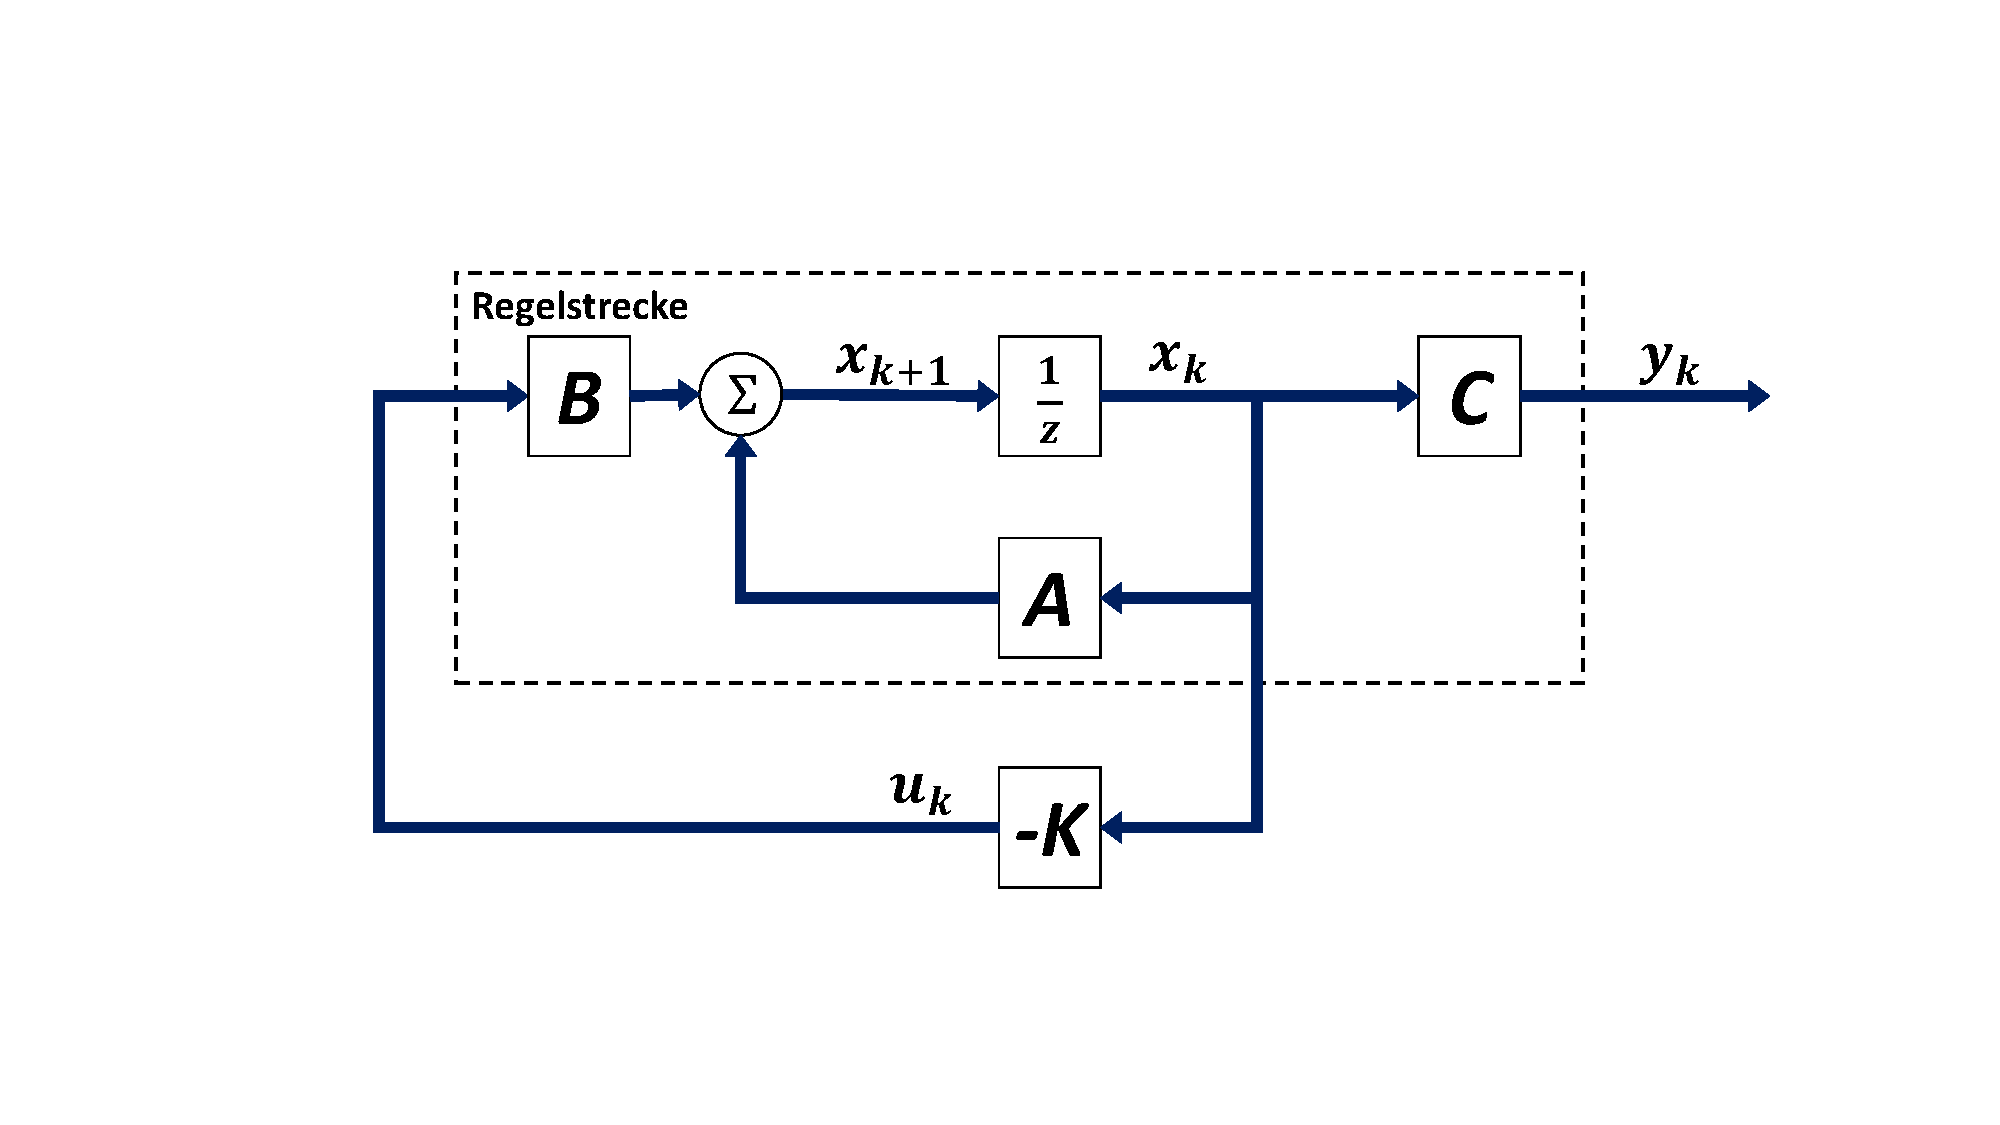
\includegraphics[width=0.8\linewidth, trim={3.5cm 3.5cm 3.5cm 3.5cm}, clip]{img/RT_ClosedLoop}
\caption{Signalfluss des geschlossenen Regelkreises, Quelle: eigene Darstellung}
\end{figure}
Aus der Abbildung gehen die Systemgleichungen des geschlossenen Regelkreises $\overline{\textfrak{D}}$($\overline{\bs{A}}$,$\bs{0}$, $\overline{\bs{C}}$) hervor.
\begin{equation}
\bs{u}(k) = -\bs{B}\bs{K}\cdot\bs{x}(k)
\end{equation}
\begin{equation}
\overline{\textfrak{D}}
: \left\{ \begin{array}{ll}
\bs{{x}}(k+1) &= \bs{A}\cdot \bs{x}(k) - \bs{B}\bs{K}\cdot \bs{x}(k) = \underbrace{(\bs{A}-\bs{B}\bs{K})}_{\equiv \bs{\overline{A}}}\cdot \bs{x}(k) \\
\bs{y}(k) &= \underbrace{\bs{C}}_{\equiv \bs{\overline{C}}}\cdot \bs{x}(k)
\end{array}
\right.
\end{equation}
Die Reglermatrix $\bs{K}$ ist nun so zu entwerfen, dass die gewünschten Eigenschaften des geschlossenen Regelkreises erreicht werden. Hierfür wird zunächst das SISO-System \dSS{A}{b}{c^T} betrachtet, wessen Systemmatrix $\bs{A}$ und Eingangsvektor $\bs{b}$ die folgende Form besitzt.
\begin{equation}
\bs{A} = \begin{bmatrix}
0 & 1 & 0 & \hdots & 0 \\
0 & 0 & 1 & \hdots & 0 \\
\vdots & \vdots & \vdots & \ddots & \vdots \\
-a\idx0 & -a\idx1 & -a\idx2 & \hdots & -a_{n-1}
\end{bmatrix}
\hspace{35pt}
\bs{b} = \begin{bmatrix}
0 \\ 0 \\ \vdots \\ 1
\end{bmatrix}
\end{equation}
Diese Darstellung heißt Regelungsnormalform und kann mittels einer Zustandstransformation erreicht werden. Diese Transformation wird hier nicht näher erläutert, da das Verfahren lediglich als Beispiel der Zustandsregelung dienen soll.\footnote{Die Bestimmung der Transformationsmatrix und der Erweiterung des Entwurfsverfahren durch Eigenwertvorgabe kann in (RT2, Lunze, S. 245) nachgelesen werden.} Der besondere Vorteil der Regelungsnormalform besteht darin, dass die Werte $a_i$ die Koeffizienten des charakteristischen Polynoms 
\begin{equation}
\text{det}(\lambda\cdot \bs{I}-\bs{A}) = \prod^n_{i=1} (\lambda-\lambda_i) = \lambda^n+a_{n-1}\cdot \lambda^{n-1} + \hdots + a\idx1\cdot \lambda + a\idx0
\end{equation}
der Systemmatrix $\bs{A}$ sind. Wird der Regelkreis über den Reglervektor
\begin{equation}
\bs{k} = \begin{bmatrix}
k_1 & k_2 & \hdots & k_n
\end{bmatrix}
\end{equation}
geschlossen, ergibt sich sich die  Systemmatrix $\bs{\overline{A}}$ des geschlossenen Regelkreises
\begin{equation}
\begin{split}
\bs{\overline{A}} = \bs{A}-\bs{b}\bs{k} &= \begin{bmatrix}
0 & 1 & 0 & \hdots & 0 \\
0 & 0 & 1 & \hdots & 0 \\
\vdots & \vdots & \vdots & \ddots & \vdots \\
-a\idx0 & -a\idx1 & -a\idx2 & \hdots & -a_{n-1}
\end{bmatrix}
-
\begin{bmatrix}
0 & 0 & 0 & \hdots & 0 \\
0 & 0 & 0 & \hdots & 0 \\
\vdots & \vdots & \vdots &  \ddots & \vdots \\
k\idx1 & k\idx2 & k\idx3 & \hdots & k_n
\end{bmatrix}
\\
&= \begin{bmatrix}
0 & 1 & 0 & \hdots & 0 \\
0 & 0 & 1 & \hdots & 0 \\
\vdots & \vdots & \vdots & \ddots & \vdots \\
-\overline{a}\idx0 & -\overline{a}\idx1 & -\overline{a}\idx2 & \hdots & -\overline{a}_{n-1}
\end{bmatrix}
\hspace{25pt} \vert \hspace{15pt} \overline{a}_i = a_i + k_{i+1} \,.
\end{split}
\end{equation}
Die Systemmatrix $\bs{\overline{A}}$ des geschlossenen Regelkreises liegt nun ebenfalls in Regelungsnormalform vor, weshalb wiederum für deren charakteristisches Polynom
\begin{equation}
\text{det}(\lambda\cdot \bs{I}-\bs{\overline{A}}) = \prod^n_{i=1} (\lambda-\overline{\lambda}_i) = \lambda^n+\overline{a}_{n-1}\cdot \lambda^{n-1} + \hdots + \overline{a}\idx1\cdot \lambda + \overline{a}\idx0
\label{eq_ew_gRK}
\end{equation}
gilt. Werden nun die Eigenwerte $\overline{\lambda}_i$ des geschlossenen Regelkreises vorgegeben können durch (\ref{eq_ew_gRK}) die Koeffizienten $\overline{a}_i$ berechnet werden. Die Koeffizienten $a_i$ der Regelstrecke werden aus der Matrix $\bs{A}$ abgelesen werden. Somit können aus der Beziehung
\begin{equation}
\overline{a}_i = a_i + k_i
\end{equation}
die einzelnen Regerfaktoren $k_i$ berechnet werden. Diese führen in dem geschlossenen Regelkreis auf die vorgegebenen Eigenwerte $\overline{\lambda}_i$. Alternativ kann auch die folgende Vektorschreibweise verwendet werden.
\begin{equation}
\underbrace{
\begin{bmatrix}
\overline{a}_0 & \overline{a}_1 & \hdots &\overline{a}_{n-1}
\end{bmatrix}}_{\equiv \bs{\overline{a}}}
=
\underbrace{
\begin{bmatrix}
a_0 & a_1 & \hdots & a_{n-1}
\end{bmatrix}}_{\equiv \bs{a}}
+
\underbrace{
\begin{bmatrix}
k_1 & k_2 & \hdots & k_n
\end{bmatrix}}_{\equiv \bs{k}}
\end{equation}
\begin{equation}
\bs{k} = \bs{\overline{a}} - \bs{a}
\end{equation}
An diesem Entwurfsverfahren werden bereits einige interessante Eigenschaften der Zustandsregelung deutlich. Zunächst können die Eigenwerte des geschlossenen Regelkreises beliebig gewählt werden wodurch das dynamische Verhalten maßgeblich bestimmt wird. Des weiteren wird der Regler durch eine Matrix-Vektor-Multiplikation realisiert. Somit werden dem Regelkreis, im Gegensatz zu PID-Reglern, keine weiteren Pole durch die Reglerdynamik hinzugefügt. Zuletzt sei die einfache Berechnung der Reglermatrix erwähnt. Sowohl die Transformation auf Regelungsnormalform als auch die Ermittlung der Regerparameter sind numerische Operationen die mit Hilfe von Matlab durchgeführt werden können.

Dennoch wird das Entwurfsverfahren in dieser Arbeit nicht verwendet. Die Gründe hierfür sind, dass das primäre Ziel darin besteht eine robuste Regelung zur Stabilisierung des Systems zu entwerfen und nicht eine spezielle Dynamik des geschlossenen Regelkreises zu erzielen. Des weiteren können bei diesem Verfahren die Verläufe der physikalischen Größen $\varphi$, $u_K$ und $u_R$ nicht direkt beeinflusst werden. Durch die Vorgabe der Eigenwerte werden lediglich die Trajektorien der kanonischen Zustandsvariablen bestimmt, welche jeweils eine Linearkombination der ursprünglichen Zustände sind. Des weiteren fließt die Stellgröße $u$ bei dieser Vorgehensweise nicht in die Bestimmung der Reglermatrix ein. Ist die Stellgröße, wie in den hier behandelten Anwendungsfällen, begrenzt müssen diese Umstände bei dem Reglerentwurf beachtet werden.

\subsection{Linear quadratisch optimale Regelung}
Im vorherigen Abschnitt wurden die Nachteile der Eigewertvorgabe aufgezeigt, weshalb hier der Entwurf eines linear quadratisch optimalen Reglers vorgestellt und an der realen Regelstrecke appliziert wird. Der Grundgedanke der optimalen Regelung ist es ein Regelgesetz zu entwerfen, welches zu einem geschlossenen Regelkreis führt, der im Sinne eines Gütekriteriums optimal ist. Hier wird das linear quadratische Gütekriterium
\begin{equation}
J = \sum^{\infty}_{k=0} \left[\bs{x}^T(k)\cdot \bs{Q} \cdot \bs{x}(k) + \bs{u}^T(k)\cdot \bs{R}\cdot \bs{u}(k)\right]
\end{equation}
verwendet. Die Matrizen $\bs{Q}$ und $\bs{R}$ dienen der Gewichtung des Zustands- bzw. Stellvektors und müssen positiv semidefinit bzw. definit sein. Durch die Gewichtungsmatrizen ist es möglich Forderung an den ursprünglichen Zustands- und Stellvektor direkt in den Reglerentwurf einfließen zu lassen. Der letztendliche Regler ergibt sich aus der Lösung des Optimierungsproblems, dass $J$ minimal wird. Nach [Ludyk, S.177] gilt für die Reglermatrix
\begin{equation}
\bs{K} = (\bs{R}+\bs{B}^T\bs{P}\bs{B})^{-1}\bs{B}^T\bs{P}\bs{A}\,,
\end{equation}
wobei $\bs{P}$ durch die Lösung der Matrix-Ricatti-Gleichung 
\begin{equation}
\bs{P} = \bs{Q}+\bs{A}^T[\bs{P}-\bs{P}\bs{B}(\bs{R}+\bs{B}^T\bs{P}\bs{B})^{-1}\bs{B}^T\bs{P}]\bs{A}
\end{equation}
bestimmt wird. Ähnlich wie bei dem Entwurf durch Eigenwertvorgabe besteht ein Vorteil der linear quadratisch optimalen Regelung darin, dass das Optimierungsproblem mittels des Matlab-Befehls \textit{dlqr()} gelöst werden kann. Somit fällt der Rechenaufwand für die Ermittlung der Reglermatrix bei der Bewertung des Entwurfverfahrens nicht weiter ins Gewicht. Deshalb werden hier lediglich die Bedeutung der Gewichtsmatrizen und die Eigenschaften des resultierenden Regelkreises diskutiert.

Hierfür müssen zunächst die Begriffe der Steuerbarkeit und Beobachtbarkeit erklärt werden. Bei einem vollständig steuerbaren System kann, durch eine passende Wahl des Stellvektors $\bs{u}$, der Zustandsvektor $\bs{x}$ in einen beliebigen Wert überführt werden. Zum Beispiel ist ein SISO-System in kanonischer Normalform mit einfachen Eigenwerten steuerbar, wenn alle Elemente $b_{i}$ des Einganvektors $\bs{\tilde{b}}$ ungleich null sind. Ist eines der Elemente $b_{i}$ gleich null kann der zugehörige Zustand $\tilde{x}_i$ nicht durch die Eingangsgröße beeinflusst werden und ist somit nicht steuerbar. Folglich kann auch dieser Eigenwert durch einen Regler nicht beeinflusst werden. Die Definition der Steuerbarkeit lautet:

\begin{quote}
\glqq Ein System $\Sigma$ heißt vollständig steuerbar, wenn es in endlicher Zeit $t_e$ von jedem beliebigen Anfangszustand $\bs{x}_0$ durch eine geeignet gewählte Eingangsgröße $\bs{u}_{[0,t_e]}$ in einen beliebig vorgegebenen Endzustand $\bs{x}(t_e)$ überführt werden kann.\grqq
\signed{LunzeRT2, S. 64}
\end{quote}

Umgekehrt beschreibt die Beobachtbarkeit die Möglichkeit den Zustandsvektor eines Systems aus dem Verlauf des Eingang- und Ausgangvektors zu rekonstruieren.

\begin{quote}
\glqq Ein System $\Sigma = (\bs{A},\bs{B},\bs{C})$ hießt vollständig beobachtbar, wenn der Anfangszustand $\bs{x}_0$ aus dem über einem endlichen Intervall $[0,t_e]$ bekannten Verlauf der Eingangsgröße $\bs{u}_{[0,t_e]}$ und der Ausgangsgröße $\bs{y}_{[0,t_e]}$ bestimmt werden kann.\grqq
\signed{LunzeRT2, S. 92}
\end{quote}

Um sowohl die Steuer- als auch Beobachtbarkeit eines Systems zu prüfen können die Kalmankritieren angewandt werden [LunzeRT2, S.93ff]. Für den Entwurf eines Zustandsregler muss ein System mindestens stabilisierbar sein. Dies bedeutet, dass alle instabilen Eingevorgänge des System sowohl steuer- als auch beobachtbar sind. Für diesen Fall lässt sich zeigen [Lunze RT2, S.301], dass der Entwurf nach dem linear qudratischen Gütekriterium zu einem asymptotisch stabilen Regelkreis führt. Hieraus folgt, dass alle Eigenwerte des geschlossenen Regelkreises im Einheitskreises liegen. Des weiteren lässt sich durch
\begin{equation}
\vert z\vert = e^{\sigma_i} \hspace{35pt} \vert \hspace{15pt} s_i = \sigma_i + \omega_i\cdot j
\end{equation}
der Abstand der Eigenwerte zum Ursprung der komplexen Ebene interpretieren. Je näher ein Eigenwert am Ursprung liegt, desto schneller wird die zugehörige Eigenbewegung. Im geschlossenen Regelkreis wird eine schnelle Systemdynamik durch hohe Stellgrößen verursacht, welche durch die Reglermatrix $\bs{K}$ bestimmt werden. Daraus folgt, dass die Erhöhung der Reglerfaktoren $k_{ij}$ die Eigenwerte des geschlossenen Regelkreises näher an den Ursprung rückt. Umgekehrt kann die Bedeutung der Gewichtungsmatrix $\bs{R}$ interpretiert werden. Je größer die Elemente von $\bs{R}$ werden, desto stärker fließt der Verlauf des Stellvektors in das Gütekriterium ein. Da dieses minimiert werden soll, resultieren kleinere Elemente der Reglermatrix und somit eine langsamere Systemdynamik.
Die Matrix $\bs{Q}$ wirkt entgegengesetzt. Da das Gütekriterium den zeitlichen Verlauf des Zustandvektors erfasst, führt eine Erhöhung der Matrix $\bs{Q}$ auf eine schnellere Eigenbewegung, welche durch erhöhte Reglerwerte erreicht wird. Hier zeigt sich ein Vorteil der linear quadratisch optimalen Regelung. Bei dem Entwurf durch Eigenwertvorgabe kann der Verlauf einer Zustandsgröße nur indirekt durch die Definition der Eigenbewegung beeinflusst werden. Im Gegensatz dazu erfolgt durch die Diagnoalelemente der Matrix $\bs{Q}$ eine direkte Gewichtung der Zustandsgrößen.\footnote{Allerdings sei angemerkt, dass sich durch die Gewichtungsmatrix $\bs{Q}$ keine Entkopplung der Zustandsgrößen erzwingen lässt. Für die Entkopplung der Zustandsgrößen müssen nicht nur die Eigenwerte sondern auch die Eigenvektoren durch den Regler beeinflusst werden. Dies ist nur möglich wenn die Reglermatrix mehr Elemente als zu regelnde Zustandsgrößen besitzt [Lunze RT2, S.254 ff]. Des weiteren sind solche System in der Realität oftmals nicht realisierbar, wären beispielsweise alle Eigenwerte und -vektoren des Würfels frei wählbar könnten die Größen $\varphi$ und $\dot{\varphi}$ voneinander entkoppelt werden.}
Da das Zeitverhalten des geschlossenen Regelkreises in dem hier behandelten Anwendungsfall eine untergeordnete Rolle spielt, wird nun die Empfindlichkeit gegenüber Störungen betrachtet. Aus dem Reglergesetzt
\begin{equation}
\bs{u} = -\bs{K}\cdot\bs{x}
\end{equation}
geht hervor, dass sich ein beliebiges Messrauschen proportional zur Reglermatrix in der Stellgröße widerspiegelt. Folglich beeinflusst das Entwurfsverfahren nicht direkt die Stör-empfindlichkeit des Regelkreises. Vielmehr wird diese durch die Lage der Eigenwerte bestimmt. Je näher diese an dem Einheitskreis liegen, desto robuster wird das System gegenüber Messrauschen.
Ein weiterer Vorteil der linear quadratisch optimalen Regelung besteht in derer Robustheit gegenüber Parameteränderungen. Diese Eigenschaft beschreibt wir groß die Abweichungen einzelner Parameter sein können um nach wie vor einen stabilen Regelkreis zu erhalten. In [Lunze RT2, S. 303ff] werden diese Eigenschaften mit Hilfe des Phasen- und Amplitudenrandes erläutert.
\newpage
\section{Erprobung des Reglers an der Regelstrecke}
Damit der Würfel auf einer Kante balancieren kann, wird ein LQ-Regler entworfen, wobei die Gewichtsmatrizen
\begin{equation}
\bs{Q} = \begin{bmatrix}
\varphi^{-2}\idx{max} & 0 & 0 \\
0 & u^{-2}\idx{K,max} & 0 \\
0 & 0 & u^{-2}\idx{R,max}
\end{bmatrix}
\hspace{35pt}
\bs{R} = \begin{bmatrix} T^{-2}\idx{M,max} \end{bmatrix}
\end{equation}
verwendet werden. Daraus resultiert das Gütekriterium
\begin{equation}
J = \sum^{\infty}_{k=0}\left( \frac{\varphi(k)^2}{\varphi^2\idx{max}} + \frac{u\idx{K}(k)^2}{u^2\idx{K,max}} + \frac{u\idx{R}(k)^2}{u^2\idx{R,max}} + \frac{T\idx{M}(k)^2}{T^2\idx{M,max}}\right)\,,
\end{equation}
in welchem der Zustandsvektor und die Stellgröße quadratisch über ihren maximalen Wert normiert werden. Die maximalen Zustandsgrößen ergeben sich aus der begrenzten Stellgröße. Beispielsweise ist das Gravitationsmoment ab dem Winkel $\varphi\idx{max}$ größer als das maximale Motormoment. 
Der geschlossene Regelkreis besitzt die Eigenwerte
\begin{equation}
\lambda_1 = 0{,}7895 \hspace{35pt} \lambda_{2,3} = 0{,}8830 \pm 0{,}0087j\,,
\end{equation}
weshalb er asymptotisch stabil ist. Im nächsten Schritt wird der Regler an der realen Regelstrecke validiert. Die folgende Abbildung zeigt den Verlauf der Zustands- und Stellgröße, wobei das System bei dem Zeitpunk $t\approx 1{,}7$ durch eine äußere Störung erregt wurde.
\begin{figure}[h!]
\centering
\includegraphics[width=0.43\textwidth]{img/edge_exp1_phi.eps}\hspace{0.7cm}
\includegraphics[width=0.43\textwidth]{img/edge_exp1_uk.eps}
\vspace{0.3cm}

\includegraphics[width=0.43\textwidth]{img/edge_exp1_ur.eps}\hspace{0.7cm}
\includegraphics[width=0.43\textwidth]{img/edge_exp1_tm.eps}\caption{Verlauf der Zustands- und Stellgrößen bei dem Versuch an der Regelstrecke}
\end{figure}
\pagebreak

Die Abbildungen zeigen, dass der Regler das System nicht in die Ruhelage $\bs{x}=\bs{0}$ überführt, sondern die Schwungmasse mit konstanter Geschwindigkeit rotieren lässt. Dieser Umstand ist darauf zurückzuführen, dass die Erfassung des Zustandsvektors von einem systematischen Messfehler betroffen ist. Im Modell wird diese Gegebenheit durch die Einführung der Zustandsgrößen
\begin{equation}
\bs{\hat{x}} = \begin{pmatrix}
\hat{\varphi} \\ \hat{u}\idx{K} \\ \hat{u}\idx{R}
\end{pmatrix}
\end{equation}
erfasst, welche die jeweiligen Messabweichungen darstellen. Der Ausgangsvektor $\bs{y}$ stellt die Messwerte dar und wird durch die Summe des ursprünglichen Zustandvektors $\bs{x}$ und der Messabweichungen $\bs{\hat{x}}$ berechnet. Aus diesen Überlegungen folgt für den offenen Regelkreis das System
\begin{equation}
\textfrak{D}\idx{o} : \left\{ \begin{split}
\bs{x}\idx{o}(k+1) &= \underbrace{\begin{bmatrix}
\bs{A} & \bs{0}^{3\times 3} \\ \bs{0}^{3\times 3} & \bs{I}^{3\times 3}\end{bmatrix}}_{\equiv \bs{A}\idx{o}}\cdot \underbrace{\begin{bmatrix}
\bs{x} \\ \bs{\hat{x}}
\end{bmatrix}}_{\equiv \bs{x}\idx{o}}(k) + \underbrace{\begin{bmatrix}
\bs{b} \\ \bs{0}^3 \end{bmatrix}}_{\equiv \bs{b}\idx{o}} \cdot u(k)
\\
\bs{y}(k) &= \underbrace{\begin{bmatrix}
\bs{I}^{3\times 3} & \bs{I}^{3\times 3}\end{bmatrix}}_{\equiv \bs{C}\idx{o}}\cdot \bs{x}\idx{o}(k)
\end{split}
\right. \,.
\end{equation}
Das Reglergesetz ergibt sich nun aus dem Produkt des Reglervektors $\bs{k}^T$ und des Ausgangsvektors $\bs{y}$
\begin{equation}
u = \bs{k}^T\cdot \bs{y} = \bs{k}^T \cdot (\bs{x} + \bs{\hat{x}}) = \underbrace{\begin{bmatrix}
\bs{k}^T & \bs{k}^T
\end{bmatrix}}_{\equiv \bs{k}^T\idx{o}} \cdot \bs{x}\idx{o} \,.
\end{equation}
Hiermit kann der Regelkreis geschlossen werden und es resultiert das System
\begin{equation}
\overline{\textfrak{D}}\idx{o} = \left\{ \begin{split}
\bs{x}\idx{o}(k+1) &= \begin{bmatrix}
\bs{A}-\bs{b}\idx{o}\bs{k}^T\idx{o} & -\bs{b}\idx{o}\bs{k}^T\idx{o} \\
\bs{0}^{3\times 3} & \bs{I}^{3\times 3}
\end{bmatrix}\cdot \bs{x}\idx{o}(k)
\\
\bs{y}(k) &= \bs{C}\idx{o}\cdot \bs{x}\idx{o}(k)
\end{split}\right.
\,.
\end{equation}
Für den geschlossenen Regelkreis ergeben sich die Eigenwerte
\begin{equation}
\lambda\idx1 = 0{,}7895 \hspace{35pt} \lambda\idx{2,3} = 0{,}8830 \pm 0{,}0087j \hspace{35pt} \lambda\idx{4,5,6} = 1
\,.
\end{equation}
Diese zeigen, dass die urpsrünglichen Eigenwerte erhalten bleiben und somit die Eigenbewegung nach wie vor stabilisiert wird. Die zusätzlichen Eigenwerte $\lambda\idx{4,5,6}=1$ sind den Messabweichungen zuzuordnen, welche als konstant modelliert wurden. Hieraus lässt sich folgern, dass der geschlossene Regelkreis als lineares System für beliebige Messabweichungen stabil ist, insofern diese nicht durch einen instabilen Vorgang verursacht werden. Um den Einfluss der Messabweichungen auf die Trajektorie $\bs{x}$ zu ermitteln wird das System $\overline{\textfrak{D}}\idx{o}$ in die kanonische Normalform transformiert.
\begin{equation}
\tilde{\overline{\bs{A}}}\idx{o} = \bs{V}^{-1}\idx{o}\overline{\bs{A}}\idx{o}\bs{V}\idx{o} = \begin{bmatrix}
\lambda\idx1 & & & \\
 & \lambda\idx2 & & \\
 & & \ddots & \\
 & & & \lambda\idx6
\end{bmatrix}
\hspace{35pt} 
\bs{x}\idx{o} = \bs{V}\idx{o}\cdot \tilde{\bs{x}}\idx{o}
\end{equation}
Interessant ist hierbei die Form der Transformationsmatrix
\begin{equation}
\renewcommand*{\arraystretch}{0.8}
\bs{V}\idx{o} = \begin{bmatrix}
\bs{V} & \begin{matrix} 0 & 0 & 0 \\ 0 & 0 & 0 \\ \gamma\idx1 & \gamma\idx2 & \gamma\idx3 \end{matrix} 
\\ \\
\bs{0}^{3\times 3} & \bs{I}^{3\times 3}
\end{bmatrix}
\,.
\end{equation}
Zunächst geht aus den unteren drei Zeilen hervor, dass es sich bei den Messabweichungen $\bs{\hat{x}}$ um kanonische Zustandsvariablen handelt. Des Weiteren bleiben die Eigenvektoren $\bs{V}$ des ursprünglichen Systems $\overline{\textfrak{D}}$ und somit auch dessen Eigenbewegung erhalten. Die Messabweichungen wirken lediglich über die Faktoren $\gamma_i$ auf die Geschwindigkeit $u\idx{R}$ des Schwungmasse ein. Unter der Annahme, dass die Messabweichungen konstant sind, führen diese zu einer verbleibenden Bewegung der Schwungmasse. Aus diesem Grund muss die vorherige Stabilitäsaussage auf das Gebiet der Zustands- und Stellgrößen begrenzt werden, für welche die Stellgröße nicht begrenzt ist. Beispielsweise kann das System nicht mehr stabilisiert werden, wenn durch einen Messfehler die maximale Drehzahl des Motors überschritten wird.

Da der Winkel $\varphi$ nach wie vor asymptotisch stabil ist, entspricht der Endwert der gemessenen Größe $\bs{y}(1)$ der Messabweichung.
\begin{equation}
\bs{y}(1) = \varphi + \hat{\varphi} \hspace{25pt} \rightarrow\hspace{25pt} \lim_{k\rightarrow\infty}\bs{y}(1) = \hat{\varphi}
\end{equation}
Deshalb wird zunächst die Messabweichung $\hat{\varphi}$ bestimmt und in einem anschließenden Versuch korrigiert. Nach dem Modell ist zu erwarten, dass die Schwungmasse beinahe zum Stillstand kommt, da lediglich die Messabweichung $\varphi$ korrigiert wird, welche allerdings den größten Einfluss auf den Endwert des Systems hat.
\begin{figure}[!ht]
\centering
\includegraphics[width=0.45\textwidth]{img/edge_exp2_phi.eps}\hspace{0.7cm}
\includegraphics[width=0.45\textwidth]{img/edge_exp2_uk.eps}
\label{plot1_edge_exp2}
\end{figure}
\begin{figure}[!ht]\ContinuedFloat
\centering
\includegraphics[width=0.45\textwidth]{img/edge_exp2_ur.eps}\hspace{0.7cm}
\includegraphics[width=0.45\textwidth]{img/edge_exp2_tm.eps}
\caption{Verlauf von $u_R$ und $T_M$ bei korrigierten Messabweichungen}
\label{plot2_edge_exp2}
\end{figure}
\newpage
Die Abbildung (\ref{plot2_edge_exp2}) zeigt den Verlauf des Systems, wobei zu dem Zeitpunkt $t=15$ die Messabweichung korrigiert wurde. Daraufhin nimmt die Geschwindigkeit $u_R$ der Schwungmasse wie erwartet ab.

\newpage
\section{Beobachtung der Messabweichungen}
Prinzipiell ist es möglich die Messabweichungen von $\varphi$ und $u_K$ empirisch zu ermitteln. Allerdings ist die Annahme, dass es sich bei den Messabweichungen um Konstanten handelt, kritisch zu betrachten. Die Ursache der Messfehler wird im Modell nicht erfasst. Werden die Größen $\bs{\hat{x}}$ von einer Zeitfunktion verursacht so werden diese ebenfalls zeitvariant. Allerdings ist die exakte Modellierung aufwendig und führt zu einer Erhöhung der Modellordnung. Um diese Problemtaik zu vermeiden wird ein Luenberger-Beobachter verwendet, welcher die Messfehler ermittelt.

Hierfür müssen zunächst die Begriffe der Steuer- und Beobachtbarkeit geklärt werden. Bei den Zustandsgrößen $\bs{\hat{x}}$ handelt es sich um so genannte nicht steuerbare Eigenvorgänge. Die Begründung liegt einerseits darin, dass die unteren drei Elemente des Eingangvektors $\bs{b}$ gleich null sind. Folglich wirkt die Stellgröße nicht direkt auf die Zustände ein. Andererseits beeinflusst keiner der Zustände $\bs{x}$ die Messabweichungen, weshalb keine indirekte Steuerung über die Stellgröße erfolgen kann. Allgemein gilt:
\begin{quote}
"\ Ein System $\Sigma$ heißt vollständig steuerbar, wenn es in endlicher Zeit $t_e$ von jedem beliebigen Anfangszustand $\bs{x}_0$ durch eine geeignet gewählte Eingangsgröße $\bs{u}_{[0,t_e]}$ in einen beliebig vorgegebenen Endzustand $\bs{x}(t_e)$ überführt werden kann."
\signed{LunzeRT2, S. 64}
\end{quote}
Zur Prüfung der Steuerbarkeit kann das Kalmankriterium angewandt werden [Lunze RT2, S.65ff]. Die nicht Steuerbarkeit der Messabweichungen begründet, weshalb kein Regler verwendet werden kann um diese zu eliminieren. Allerdings sind diese beobachtbar. Das heißt sie können aus dem Verlauf des Ausgangs- und Stellvektors rekonstruiert werden.
\begin{quote}
"\ Ein System $\Sigma = (\bs{A},\bs{B},\bs{C})$ hießt vollständig beobachtbar, wenn der Anfangszustand $\bs{x}_0$ aus dem über einem endlichen Intervall $[0,t_e]$ bekannten Verlauf der Eingangsgröße $\bs{u}_{[0,t_e]}$ und der Ausgangsgröße $\bs{y}_{[0,t_e]}$ bestimmt werden kann. "
\signed{LunzeRT2, S. 92}
\end{quote}
Zu der Prüfung der Beobachtbarkeit kann ebenfalls das Kalmankriterium genutzt werden [LunzeRT2, S.93ff]. Da das System $\overline{\textfrak{D}}_o$ vollständig beobachtbar ist, kann ein Luenberger-Beobachter verwendet werden um den Zustandsvektor $\bs{x}_o$ zu schätzen. Das Grundprizip der Beobachtung besteht darin, parallel zu der Regelstrecke das Modell zu berechnen und daraus den Zustandsvektor zu schätzen. Die Problematik dieses Ansatz besteht darin, dass ein beliebiger Modellfehler zu einem, mit der Zeit zunehmenden, Schätzfehler führt. Deshalb wir das in der Regelungstechnik bewährte Prinzip der Fehlerrückführung übernommen. Da der Zustandsvektor $\bs{x}$ der Regelstrecke nicht zur Verfügung steht wird die Differenz
\begin{equation}
\delta\bs{y} = \bs{y} - \bs{\hat{y}}
\end{equation}
der Ausgangsgrößen berechnet. Diese fließt über die Beobachtermatrix $\bs{L}$ in den Schätzwert $\bs{\hat{x}}$ des Zustandes ein.

BILD

Um das Verhalten des Beobachters zu untersuchen wird der Schätzfehler $\bs{e} = \bs{x} - \bs{\hat{x}}$ betrachtet.
\begin{equation}
\begin{split}
\bs{e}(k+1) &= \bs{x}(k+1) - \bs{\hat{x}}(k+1) \\
&= [\bs{A}\cdot \bs{x}(k) + \bs{B}\cdot \bs{u}(k)] - [\bs{A}\cdot \bs{\hat{x}}(k) + \bs{B}\cdot \bs{u}(k) +\bs{L}\bs{\hat{y}}(k)]
\\
&= [\bs{A}\cdot (\bs{x}(k) - \bs{\hat{x}}(k))] - \bs{L}\bs{C}\cdot[\bs{x}(k)-\bs{\hat{x}}(k)] 
\\
&= \bs{A}\cdot \bs{e}(k) - \bs{LC}\cdot\bs{e}(k) = (\bs{A}-\bs{LC})\cdot \bs{e}(k)
\end{split}
\end{equation}

\ifx\FORMAT\undefined
\end{document}
\fi


\ifx\FORMAT\undefined
\documentclass[11pt]{book}
\usepackage{amsmath,mathtools}
\usepackage[utf8]{inputenc}
\usepackage[ngerman]{babel}
\usepackage{acronym}
\usepackage{graphicx} 
\usepackage{epstopdf}
\usepackage{svg}
\usepackage{multirow}
\usepackage{amssymb}
\usepackage{trfsigns}
\usepackage{setspace}
\usepackage{yfonts}
%\usepackage{HsKatitle11}

\onehalfspacing


%Hyperlinks package, links aus inhaltsverzeichnis
\usepackage{hyperref}
\hypersetup{
    colorlinks=false, %set true if you want colored links
    linktoc=all,
    linkbordercolor = {white}
}
%Blattformatierung
\usepackage{geometry}
\geometry{a4paper, top=25mm, left=30mm, right=25mm, bottom=20mm}

%Listing
\usepackage{courier}
\usepackage{listings}
\usepackage{color}
 \lstset{
   frame=tb,
   framexleftmargin=2.5em,
   basicstyle=\small\linespread{0.9}\bfseries\ttfamily,
   emph={square}, 
   emphstyle=\color{blue}\texttt,
   emph={[2]root,base},
   emphstyle={[2]\color{yac}\texttt},
   showstringspaces=false,
   flexiblecolumns=false,
   tabsize=2,
   numbers=left,
   numberstyle=\small\bfseries\ttfamily,
   numberblanklines=false,
   stepnumber=1,
   numbersep=10pt,
   xleftmargin=25pt
 }
 
 \def\presuper#1#2%
	{\mathop{}%
	\mathopen{\vphantom{#2}}^{#1}%
	\kern-\scriptspace%
	#2}
%Display vecotr in a reference frame
\newcommand{\vecBS}[4]{\presuper{#1}{\begin{pmatrix}
#2 \\ #3 \\ #4
\end{pmatrix}}}
%Boldsymbol shortcut
\newcommand{\bs}[1]{\boldsymbol{#1}}
%Bezugssystemdefinition
\newcommand{\defBS}[1]{\{#1\} [ \bs{e}_{{#1}_1},\bs{e}_{{#1}_2}, \bs{e}_{{#1}_3} ]}
%Projektionsmatrix
\newcommand{\pMat}[2]{\presuper{#1}{\bs{P}}^{#2}}
%Differenation in Respekt zu BS
\newcommand{\diffIn}[3]{\frac{\presuper{#1}{d{#2}}}{d#3}}
\newcommand{\partialDiffIn}[3]{\frac{\presuper{#1}{\partial{#2}}}{\partial #3}}
%Geschwindigkeit/Beschleunigung
\newcommand{\vel}[3]{\presuper{#1}{\bs{#2}}^{#3}}

%Rightarrow with spaceing
\newcommand{\rArrow}{\hspace{5pt}\rightarrow\hspace{5pt}}
%Inneres Produkt
\newcommand{\inProd}[2]{\langle {#1}, {#2} \rangle}

%System macro
\newcommand{\cSS}[3]{\textfrak{S}($\bs{#1}$,$\bs{#2}$,$\bs{#3}$)}
\newcommand{\dSS}[3]{\textfrak{D}($\bs{#1}$,$\bs{#2}$,$\bs{#3}$)}

%Laplace transform sign with spaces
\newcommand{\myLaplace}{\hspace{15pt}\laplace\hspace{15pt}}

\newcommand*{\signed}[1]{%
        \nolinebreak[3]\hspace*{\fill}\mbox{\emph{#1}}
    }
\begin{document}
\fi

\chapter{Software}
Wie bereits in den letzten Abschnitten erläutert wird der Regler als diskretes System implementiert. Deshalb spielt die verwendete Hardware und darauf ausgeführte Software eine zentrale Rolle. Dieser Umstand wird dadurch verstärkt, dass sämtliche Versuche, wie z.B. die Justierung der Sensoren, Systemidentifikation und Erprobung verschiedener Reglerkonzepte, in Form eines Programms durchgeführt werden. Aus diesem Grund widmet sich dieser Abschnitt dem Aufbau einer Software-Infrastruktur, welche die effiziente Entwicklung von mechatronischen Anwendungen ermöglicht.

\newpage
\section{Zielplattform, Sensorik und Aktorik}
In diesem Projekt wird ein BeagleBone Black\footnote{Im weiteren wird die Kurzform BeagleBone bzw. die Abkürzung BBB verwendet.} \cite{BBBSRM} in Kombination mit einer Linux-Distribution verwendet um die digitale Regelung zu realisieren. Die Plattform basiert auf einem AM335x Sitara  Prozessor \cite{AM335x}, der mit einer Taktrate von 1GHz betrieben wird. Des weiteren steht eine single precision NEON FPU, für die Berechnung von Gleitkommaoperationen, zur Verfügung. Diese Plattform reduziert die nötige Rechenzeit für gewöhnliche Filter- und Regelungsalgorithmen auf wenige Mikrosekunden. Somit kann die durch die Berechnung resultierende Totzeitbei dem Reglerentwurf vernachlässigt werden.
Das Linux-Betriebssystem bringt weitere Vorteile für die Entwicklung des Gesamtsystems mit sich. Zunächst existiert eine Vielzahl von Werkzeugen für die Entwicklung von Embbeded-Linux-Anwendungen. Dadurch wird der nötige Zeitaufwand für die Implementierung des Reglerprogramms reduziert. Des weiteren kann bei der Entwicklung auf Pakete und Bibliotheken der Linux-Gemeinde zurückgegriffen werden. Somit können auch komplexe Subsysteme, wie z.B. der hier verwendete TCP/IP-Server, in das Gesamtsystem eingebettet werden. Zuletzt kann das Dateisystem genutzt werden um Konfigurationen für Filter- und Regleralgorithmen auszutauschen, wodurch die Erprobung von verschiedenen Reglerkonzepten vereinfacht wird. 
Allerdings muss der Einfluss des Betriebssystem auf das Zeitverhalten der Regelung kritisch betrachtet werden. Einerseits kann die Abtastung an äquidistanten Stützstellen nicht mehr garantiert werden. Anderseits entsteht durch die Verwendung von Linux-Treibern Verzögerungen, die zu weiteren Totzeiten führen.

Aus diesem Grund wird zunächst die verwendete Peripherie und deren softwareseite Auswertung vorgestellt. Auf dem Würfelgehäuse sind insgesamt sechs MPU9250-Module \cite{MPU9250} montiert. Die Module besitzen jeweils einen Beschleunigungs- und Drehratensensor, welche genutzt werden um einen Teil des Zustandvektors zu bestimmen. Die Kommunikation zwischen den Sensormodulen und dem BeagleBone Black erfolgt über einen SPI-Bus. Das das SPI-Modul des BeagleBone Black nur einen CS-Pin besitzt, wird dieser über einen Analogschalter \cite{MAX4617} mit den Sensoren verbunden.
\begin{figure}[!h]
\centering
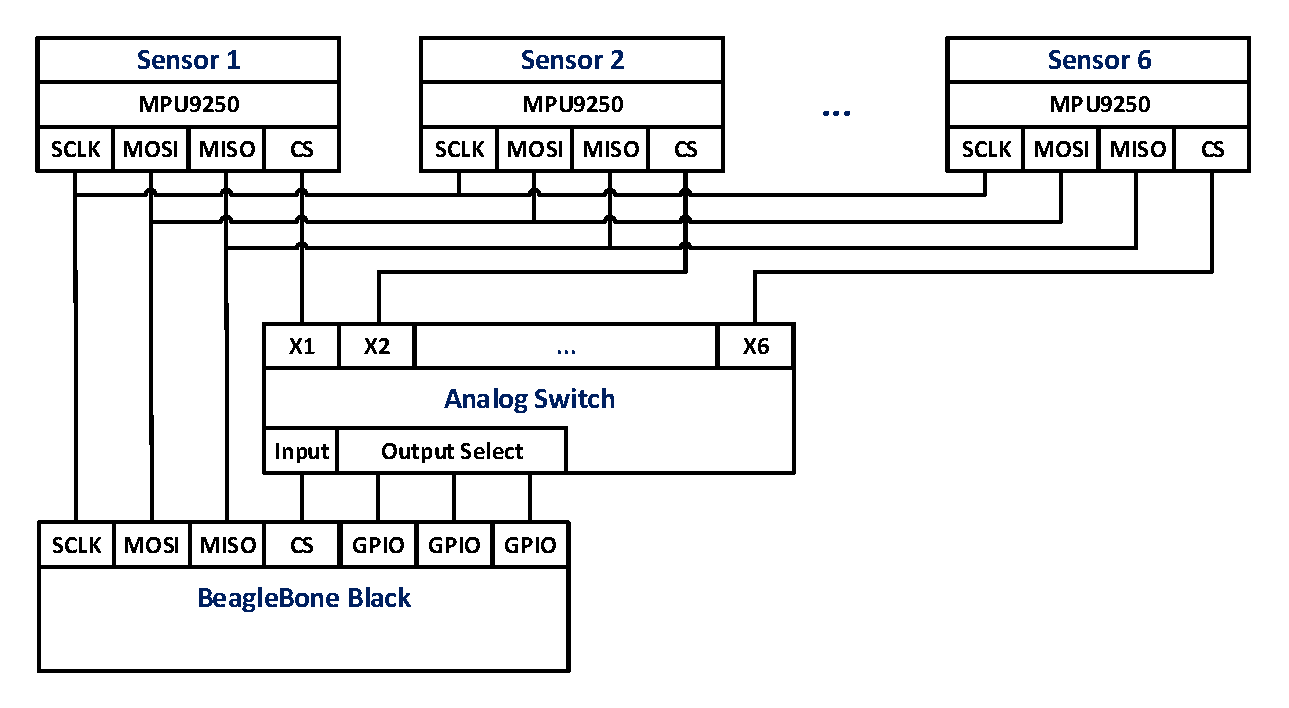
\includegraphics[width=0.7\linewidth]{img/SW_0_Sensoren_BSB.pdf}
\caption{Blockschaltbild Sensorkommunikation}
\end{figure}
Drei digitale Ausgänge des BealgeBone sind mit den Steuereingängen des Schalters verbunden um die CS-Leitung auf den Ausgang des gewünschten Sensors zu legen.
Im Quellcode werden die Peripheriegeräte durch Klassen repräsentiert. Für die Steuerung der Digitalausgänge wird die Klasse \textit{CGPIO} implementiert, welche als Konstruktorargument die Nummer des zu konfigurierenden Pins entgegennimmt. Des weiteren bietet sie Methoden zum Setzen bzw. Rücksetzen des Ausgangs. Hierfür wird die Schnittstelle des Treibers im Dateisystem verwendet. Zur Steuerung des Schalters wird die Klasse \textit{CSwitch} aus drei Instanzen des Typs \textit{CGPIO} komponiert und implementiert die Methoden \textit{selectXi()} um die Schalterausgänge auszuwählen.
Analog wird für die Konfiguration und Auswertung der Sensoren die Klasse \textit{CMPU9250} implementiert. Zur Interaktion mit dem SPI-Treiber wird die Posix-Funktion \textit{ioctl()} verwendet, welche zu einer kürzeren Ausführungszeit der Treiberaufrufe führt und im Vergleich zu der Dateisystemschnittstelle detaillierte Konfigurationsoptionen bietet. Die Klasse nutzt die SPI-Schnittstelle um die Sensoren in der \textit{init()}-Methode zu konfigurieren. Anschießend können über die Methode \textit{fetchData()} die aktuellen Beschleunigungs- und Winkelgeschwindigkeitswerte ausgelesen werden.

Die letztendliche Anwenderschnittstelle bietet die Klasse \textit{CSensorSystem}, welche aus einer Instanz des Typ \textit{CSwitch} und \textit{CMPU9250} komponiert wird. Im Konstruktur werden die sechs Sensoren initialisiert und anschließend über die Methode \textit{fetchSensorData()} ausgelesen. Die Daten werden in der Struktur \textit{SSensorData} gespeichert, welche Membervariablen für die Messwerte besitzt.
\begin{figure}[!h]
\centering
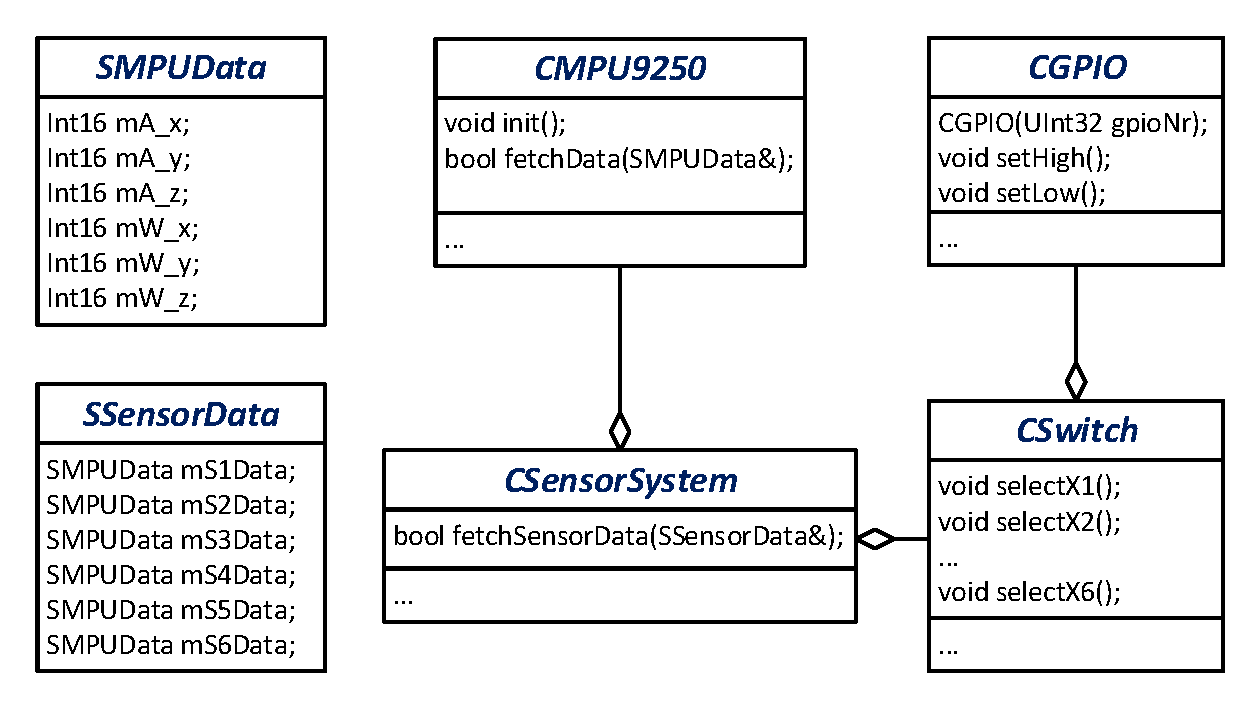
\includegraphics[width=0.7\linewidth]{img/SW_0_Sensoren_KD.pdf}
\caption{Klassendiagramm der Sensorschnittstelle}
\end{figure}

Die Stellgrößen der Regelung werden durch drei Motoren generiert, die jeweils über einen Treiberbaustein kontrolliert werden. Jeder Motortreiber ist mit zwei digitalen Ausgängen verbunden. Diese steuern die Freigabe und Drehrichtung des Motors. Die Vorgabe des Drehmoments erfolgt über ein PWM-Signal. Zusätzlich erfassen die Motortreiber die Drehzahl und geben diese in Form eines Analogsignals an das BeagleBone zurück.
\begin{figure}[!h]
\centering
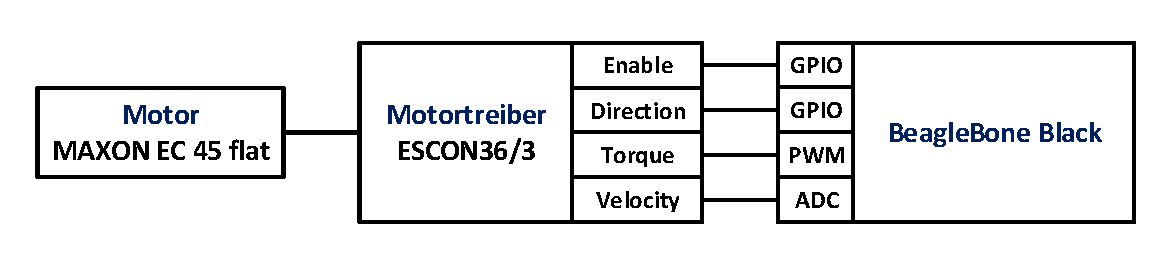
\includegraphics[width=0.7\linewidth]{img/SW_0_Motoren_BSB.pdf}
\caption{Blockschaltbild der Motoransteuerung} 
\end{figure}
Die Klasse \textit{CPWM} ermöglicht das Setzen eines Duty-Cycles, wobei die Treiberschnittstelle im Dateisystem verwendet wird. Eine Instanz dieser Klasse wird in \textit{CMotor} genutzt um das gewünschte Drehmoment einzustellen. Des weiteren werden zwei Instanz von \textit{CGPIO} genutzt um die Freigabe und Drehrichtung des Motors einzustellen. Für das Auslesen der ADC-Werte wird ebenfalls eine Klasse \textit{CADC} angelegt. Da der Linux-Treiber für die Nutzung der AD-Wandler teilweise fehlerhaft ist wird ein alternative Vorgehensweise zur Nutzung der Peripherie genutzt. Hierbei wird mittels der Posix-Funktion \textit{mmap()} der Adressbereich der ADC-Peripherie in den Userspace gelegt. Dadurch kann in der Anwendung direkt auf die ADC-Register zugegriffen werden. Durch diesen Ansatz ergeben sich zwei Vorteile. Einerseits werden dem Nutzer keine Einschränkungen durch die Treiberschnittstelle aufgezwungen. Andererseits wird die nötige Zeit der AD-Wandlung durch den direkten Zugriff auf die Register reduziert. Allerdings ist diese Vorgehensweise mit einem größeren Implementierungsaufwand verbunden und wird deshalb nur genutzt wenn die Einschränkungen des Treibers nicht annehmbar sind.
die Klasse \textit{CSensorSystem} wird um eine Instanz von \textit{CADC} erweitert und umfasst somit die vollständige Sensorik des Systems. Um die Peripherie vollständig zu kapseln wird die Klasse \textit{CHardware} aus einer Instanz von \textit{CMotor} und \textit{CSensorSystem} komponiert.
\begin{figure}[!h]
\centering
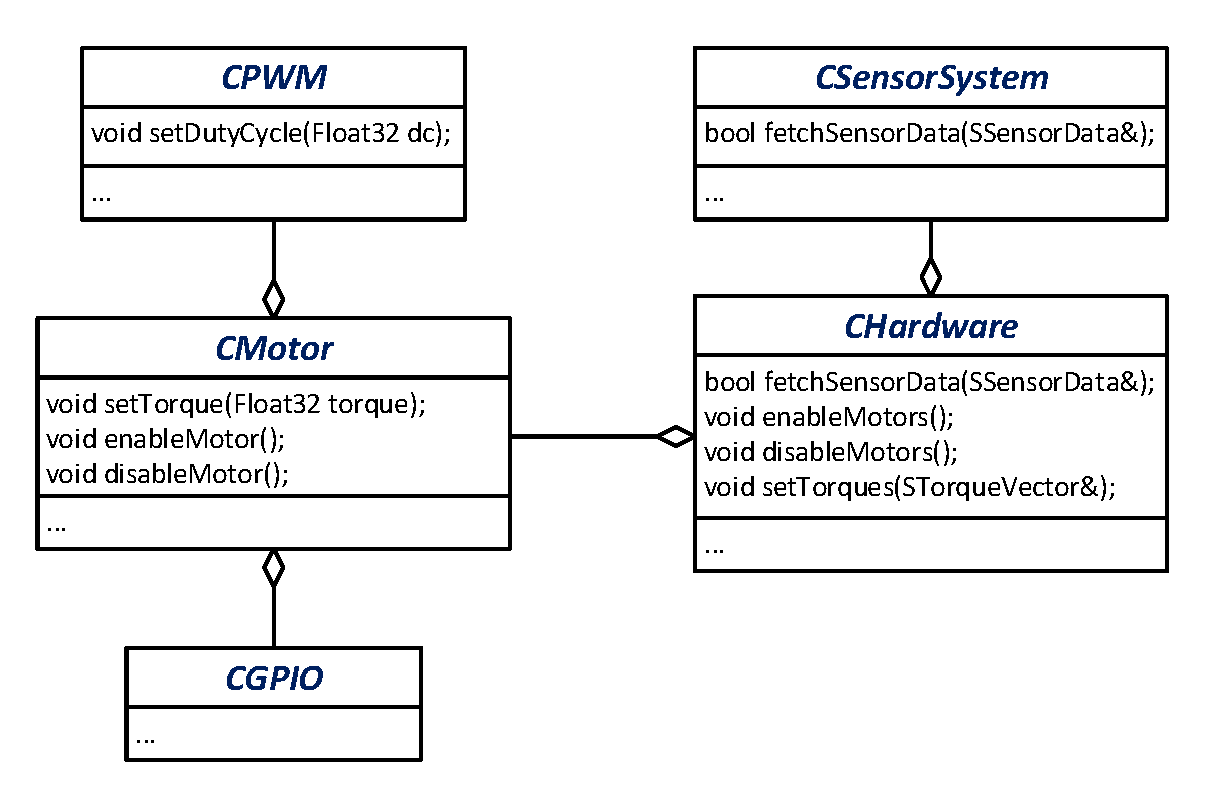
\includegraphics[width=0.7\linewidth]{img/SW_0_Hardware_KD.pdf}
\caption{Klassendiagramm der Hardwareansteuerung}
\end{figure}
\newpage
\section{Implementierung des Signalflusses}
Im nächsten Schritt muss der Signalfluss implementiert werden. Hierfür wird ein Ansatz der Template-Metaprogrammierung verwendet, um ein einheitliches Konzept für die Umsetzung von Singalverarbeitungsalgorithmen zu schaffen. Ebenso soll das Konzept Änderung im Singalfluss ermöglichen, ohne dabei größere Eingriffe im Quellcode vornehmen zu müssen. Als Beispiel wird das folgende Blockschaltbild verwendet.
Zunächst wird eine, auf den Sensorwerten basierende, Zustandsschätzung durchgeführt. Dieser Vektor wird anschließend gefiltert und zur Berechnung des Reglers genutzt.
\begin{figure}[!h]
\centering
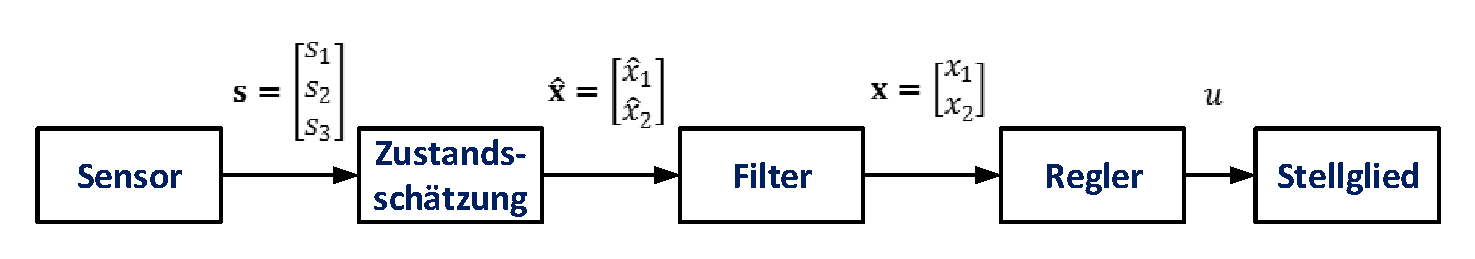
\includegraphics[width=0.9\linewidth, trim={0cm 0cm 0cm 14cm}, clip]{img/SW_1_Signalfluss_BSB.pdf}
\caption{Blockschaltbild des Signalflusses}
\end{figure}

Für die Implementierung werden die Signale als Datenobjekte implementiert. Das heißt es werden Strukturen oder Klassen entworfen, welche die Daten enthalten und ggf. Methoden für den Zugriff oder Bearbeitung bieten. Für dieses Beispiel repräsentieren die Strukturen \textit{SSensorData} und \textit{SStateVector} den Sensor- bzw. Zustandsvektor. Für die Modellierung der Stellgröße genügt eine \textit{float}-Variable.
\begin{lstlisting}[caption={Beispielhafte Implementierung eines Datenobjektes},captionpos=b]
struct SSensorData
{
	Float32 mS1;
	Float32 mS2;
	Float32 mS3;
};
struct SStateVector
{
	Float32 mX1;
	Float32 mX2;
};
using UType = Float32;
\end{lstlisting}
Die Systeme im Signalfluss werden als Klassen implementiert, die als Aktionsobjekte bezeichnet werden. Die Klassen werden nach dem folgenden Schema entworfen, wobei als Beispiel ein Objekt zur Zustandsschätzung aufgezeigt wird.
\begin{lstlisting}[caption={Beispielhafte Implementierung eines Aktionsobjektes},captionpos=b]
class CStateEstimate
{
public:
	using InputType	 = SSensorData;
	using OutputType = SStateVector;
public:
	const OutputType& calcOutput(const InputType& input);
	const OutputType& getValue() const;
	...
private:	 
	OutputType mOutput;
};
\end{lstlisting}
Die Aktionsobjekte definieren zunächst ihren Ein- und Ausgangstyp. Die Berechnung des Systems erfolgt über die Methode \textit{calcOutput()}.
Nun müssen die Aktionsobjekte zu dem vorgegebenen Signalfluss zusammengefasst werden. Um diesen Schritt im Entwicklungsprozess zu erleichtern, soll ein Konzept implementiert werden, dem eine Typenliste der Aktionsobjekte übergeben wird und daraus das Blockschaltbild erzeugt.
Für die Implementierung der Typenliste wird der Ansatz nach \cite[S. 40 ff.]{ModernCpp} verwendet. Zunächst wird die leere Struktur \textit{CNullType} definiert, welche als Terminierungssymbol in der Typenliste fungiert. Die Liste wird mit Hilfe der Templatestruktur \textit{TTypeList} implementiert, welche als Parameter einen Anfangs- und Endtypen entgegennimmt.
\begin{lstlisting}[caption={Implementierung der Typenlist},captionpos=b]
struct CNullType{};

template<class HeadType, class TailType>
struct TTypeList
{
	using Head = HeadType;
	using Tail = TailType;
};
\end{lstlisting}
Die obige Implementierung unterstützt lediglich Listen der Länge zwei. Deshalb werden Makros verwendet \cite[S. 45]{ModernCpp}, die rekursive Intanszierungen des Templates nutzen um die Listen beliebiger Länge zu erhalten. Mittels dieser Makros kann dann auch die Typenliste der Aktionsobjekte erzeugt werden.
\begin{lstlisting}[caption={Definition und Aufruf der Makors für verlängerte Typenlisten},captionpos=b]
#define TYPELIST_1(T1)         TTypeList<T1, CNullType>
#define TYPELIST_2(T1, T2) 	   TTypeList<T1, TYPELIST_1(T2)>
#define TYPELIST_3(T1, T2, T3) TTypeList<T1, TYPELIST_2(T2, T3)>
...
using ActionObjList = TYPELIST_3(CStateEstimate, CFilter, CController);
\end{lstlisting}
Um nun die Aktionstypen zu einem Signalfluss-Objekt zusammenzufügen, wird das Muster der linearen Typenhierachie nach \cite[S. 62 ff.]{ModernCpp} angewandt. Dessen Aufbau erinnert an eine verkettete Liste, wobei die Typen durch Vererbung verknüpft werden. Die Templateklasse \textit{TActionHolder} wird als Träger für die Aktionsobjekte entworfen.
Im allgemeinen Fall wird dem Template der Typ eines Aktionobjektes \textit{ActionObj} und eine beliebige Elternklasse \textit{Base} übergeben, die beide an \textit{TActionHolder} vererben. In der \textit{calcOutput()}-Methode wird zunächst die Berechnung des Aktionsobjektes durchgeführt und anschließend \textit{calcOutput()} der zweiten Elternklasse aufgerufen.
\begin{lstlisting}[caption={Templateklasse des Trägerobjektes},captionpos=b]
template<class ActionObj, class Base>
class TActionHolder : public Base, public ActionObj
{
public:
	void calcOutput(const ActionObj::InputType& input)
	{
		ActionObj::calcOutput(input);
		Base::calcOutput(ActionObj::getValue());
	}
};
\end{lstlisting}
Des weiteren besteht eine Templatespezialisierung für den Fall, dass ein Aktionstyp und \textit{CNullType}, der das Ende der Typenliste signalisiert, übergeben werden. Nun wird in der \textit{calcOutput()}-Methode lediglich das Aktionsobjekt berechnet, da das Ende der Typenliste und somit des Signalflusses erreicht ist.
\begin{lstlisting}[caption={Templatespezialisierung des Trägerobjektes für das Ende der Typenliste},captionpos=b]
template<class ActionObj>
class TActionHodler<ActionObj, CNullType> : 
	public CNullType, public ActionObj
{
public:
	void calcOutput(const ActionObj::InputType& input)
	{
		ActionObj::calcOutput(input);
	}
};
\end{lstlisting}
Die zweite Templateklasse ist \textit{TLinHierachy}, mit dem folgenden Prototyp.
\begin{lstlisting}[caption={Deklaration der Templateklasse für lineare Hierarchien {\cite[S. 63]{ModernCpp}} },captionpos=b]
template<class TList,
         template<AtomicType, class Base> class Unit,
         class Root = CNullType>
class TLinHierachy;
\end{lstlisting} 
Der erste Templateparameter ist die Typenliste, welche die zu generierende Typenhierachie vorgibt. Der zweite Parameter ist eine Templateklasse, die als Träger der Objekte aus der Typenliste agiert. In diesem Anwendungsfall wird die zuvor definierte Templateklasse \textit{TActionHolder} verwendet. Der letzte Parameter ist der Terminierungstyp der Hierarchie, welcher als Standardargument \textit{CNullType} übergeben wird. Analog zu \textit{TActionHolder} werden durch Spezialisierungen zwei Fälle unterschieden. Zunächst sei der Fall betrachtet, dass der Parameter \textit{TList} eine Typenliste aus zwei beliebigen Typen ist.
\begin{lstlisting}[caption={Erste Templatespezialisierung der linearen Hierarchie {\cite[S. 64]{ModernCpp}} },captionpos=b]
template<class T1, 
         class T2, 
         template<class, class> class Unit, 
         class Root>
class TLinHierachy<TTypeList<T1, T2>, Unit, Root>
	: public Unit<T1, TLinHierachy<T2, Unit, Root> >
{};
\end{lstlisting}
Diese Instanziierung wird solange genutzt bist das Ende der ursprünglichen Typenliste erreicht ist. Die instantiierte Klasse von \textit{TLinHierachy}, ist eine leere Klasse die von \textit{Unit} erbt. \textit{Unit} wird wiederum mit \textit{TLinHierachy} instantiiert, wobei lediglich der zweite Parameter \textit{T2} übergeben wird. Dadurch wird die ursprüngliche Typenliste schrittweise abgearbeitet.
Die zweite Templatespezialisierung wird genutzt um die Generation am Ende der Typenliste zu terminieren. Dies ist der Fall wenn \textit{TLinHierachy} mit einer Typeliste der Länge eins instantiiert wird.
\begin{lstlisting}[caption={Zweite Templatespezialisierung der linearen Hierarchie {\cite[S. 64]{ModernCpp}} },captionpos=b]
template<class T, template<class, class> class Unit, class Root>
class TLinHierachy<TYPELIST_1(T), Unit, Root>
	: public Unit<T, Root>
{};
\end{lstlisting}
Für das hier aufgeführte Beispiel ergibt sich die folgende Vererbungshierarchie.
\begin{figure}[!h]
\centering
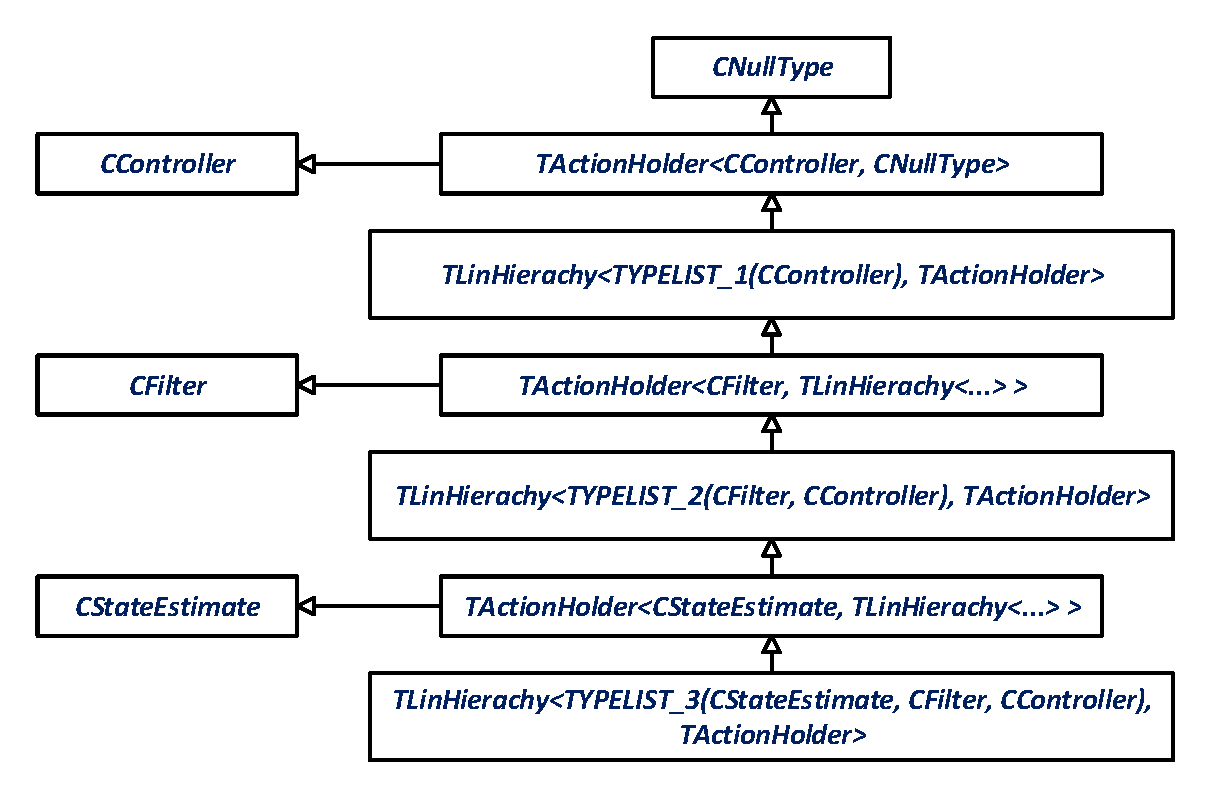
\includegraphics[width=0.7\linewidth]{img/SW_1_Signalfluss_KD.pdf}
\caption{Klassendiagramm der generierten Hierarchie}
\end{figure}
Der Vorteil dieses Konzept, welches mit einem nicht zu vernachlässigenden Programmieraufwand verbunden ist, zeigt sich bei der letztendlichen Nutzung. Sind die Aktionsobjekte definiert können sie in wenigen Zeilen zu dem Signalfluss zusammengesetzt werden.
\begin{lstlisting}[caption={Anwendungsbeispiel der linearen Hierarchie},captionpos=b]
using ActionList = TYPELIST_3(CStateEstimate, CFilter, CController);
using SignalFlow = TLinHierachy<ActionList, TActionHandler>;
SignalFlow mySF;
\end{lstlisting}
Sollen nun im Projektverlauf einzelne Elemente ausgetauscht oder erweitert werden muss lediglich die Typendefinition von \textit{ActionList} geändert werden. Da die Hierarchie mittels Vererbung realisiert wird, können durch die Angabe des Namensraum die Methoden aller Elternklassen verwendet werden. Beispielsweise zeigt der folgende Ausschnitt die Abfrage aller berechneten Signale.
\begin{lstlisting}[caption={Beispiel für den Zugriff auf Aktionsobjekte in der Hierarchie},captionpos=b]
SStateVector x_estimate = mySF.CStateEstimate::getValue();
SStateVector x_filtered = mySF.CFilter::getValue();
UType        u          = mySF.CController::getValue();
\end{lstlisting}
Ebenso können zur Laufzeit konfigurierbare Elemente oder Verzweigungen implementiert werden. Angenommen zur Filterung sollen entweder ein Komplementär-Filter (\textit{CCompFilter}) oder ein Tiefpass erster Ordnung (\textit{CPT1}) genutzt werden. Dann kann eine Klasse \textit{CFilterSystem} aus diesen beiden komponiert werden, die zusätzliche Methoden zur Filterauswahl bietet.
\begin{lstlisting}[caption={Beispiel für die komponierte Aktionsobjekte},captionpos=b]
class CFilterSystem
{
public:
	using InputType  = SStateVector;
	using OutputType = SStateVector;
public:
	const OutputType& calcOutput(const InputType& input)
	{
		mCompFilter.calcOutput(input);
		mPT1Filter.calcOutput(input);
		
		return this->getValue();
	}
	const OutputType& getValue()
	{
		switch(mActiveFilter)
		{
			case EFilter::CompFilter:
				return mCompFilter.getValue();
			case EFilter::PT1Filter:
				return mPT1Filter.getValue();
			default:
				return input;
		}
	}
	void setFilter(EFilter filter)
	{
		mActiveFilter = filter;
	}
private:
	CCompFilter mCompFilter;
	CPT1        mPT1Filter;
	EFilter     mActiveFilter;
};
\end{lstlisting}
Analog können auch komplexere Verzweigungen realisiert werden, wobei \textit{TLinHierachy} zur Generation von Teilzweigen des Blockschaltbildes verwendet werden kann.
\newpage
\section{Aufbau der Komponentenarchitektur}
In dem letzten Abschnitt wurden die elementaren Funktionen des Regelkreises, wie die Peripherieinteraktion und der Signalfluss, implementiert. Um eine effiziente Versuchsdurchführung zu ermöglichen müssen allerdings weitere Funktionalitäten bereitstehen. Einerseits müssen einzelne Elemente des Regelkreises während der Ausführung konfigurierbar sein. Beispielsweise soll zwischen unterschiedlichen Regler umgeschaltet werden und einzelne Parameter geändert werden können. Des weiteren müssen die gemessen und berechneten Werte des Signalflusses an einen Entwicklungsrechner übertragen werden. Dort werden die Daten visualisiert und für eine spätere Analyse gespeichert.
Folglich muss ein Kommunikationskonzept implementiert werden um Daten zwischen der Ziel- und Entwicklungsplattform auszutauschen. Um die Berechnung des Regelkreises und die Kommunikationsaufgaben voneinander zu trennen wird eine Komponentenarchitektur eingeführt (\cite{Wietzke1}, S. 279 ff.). Die erste Komponente, welche als Regelungskomponente bezeichnet wird, führt die Berechnung des Signalflusses und die Interaktion mit den Peripheriegeräten durch. Des weiteren übernimmt sie die logische Steuerung der Versuchsabläufe. Die Kommunikationskomponente ist für die Verbindung mit dem Entwicklungsrechner verantwortlich und ermöglicht den Datenaustausch zwischen den beiden Plattform. Hierfür wird ein TCP/IP-Server verwendet.
\begin{figure}[!h]
\centering
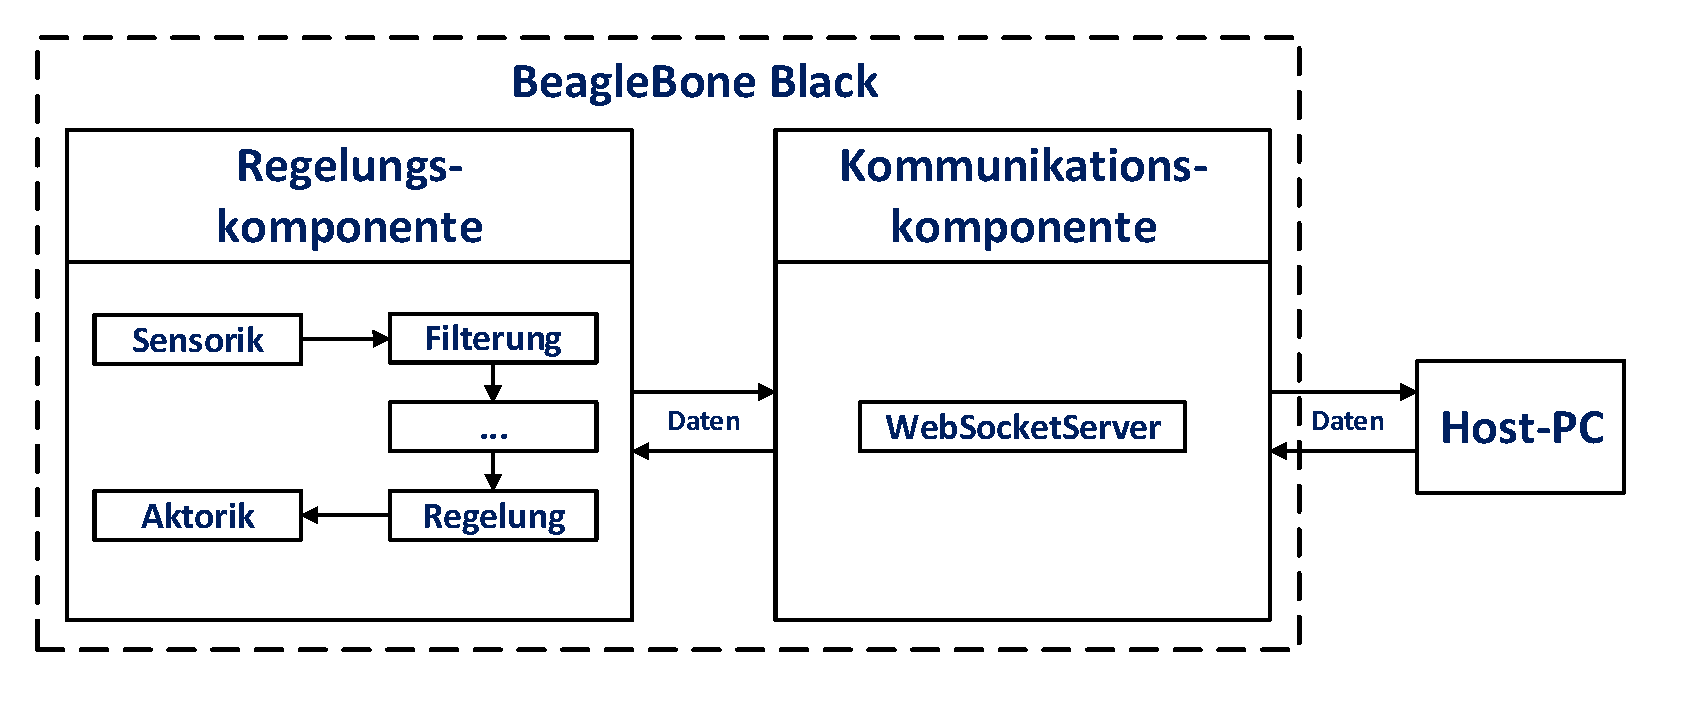
\includegraphics[width=\linewidth]{img/SW_1_KA_BSB.pdf}
\caption{Blockschaltbild Gesamtsystem}
\end{figure}
Durch die Verwendung der Komponentenarchitektur entstehen einige Vorteile. Zunächst können die beiden Komponenten in unterschiedlichen Threads ausgeführt werden. Dadurch wird die Bearbeitung der beiden Aufgabenbereiche zum Großteil entkoppelt. Der Datenaustausch zwischen den Komponenten reduziert sich auf eine kontrollierte Schnittstelle, wodurch die Fehleranfälligkeit des Gesamtsystems minimiert wird. Des weiteren können die Aufgaben priorisiert werden, da der Scheduler eine preemptive Round-Robin-Strategie verfolgt (\cite{Wietzke1}, S. 19). Somit kann die Ausführung der Regelungskomponente, welche für die Bearbeitung der zeit- und sicherheitsrelevanten Aufgaben zuständig ist, gegenüber der Kommunikationseinheit priorisiert werden. Hieraus resultiert, dass das Zeitverhalten der Regelung als deterministisch angenommen werden kann. 

Für die Implementierung wird das Interface \textit{IRunnable} definiert, welches virtuelle Methoden zur Initialisierung und Ausführung der Komponenten vorschreibt. Diese Schnittstelle wird von der abstrakten Klasse \textit{AComponentBase} geerbt, welche Membervariablen zum Datenaustausch besitzt. Die letzendlichen Komponenten werden in Form der beiden Klassen \textit{CControlComp} und \textit{CCommComp} realisiert. Die Erzeugung der Threads erfolgt mit Hilfe der Klasse \textit{CThread}, deren Instanz als Trägerobjekte der Threads agieren (\cite{Wietzke1}, S. 108 ff.).
\begin{figure}[!h]
\centering
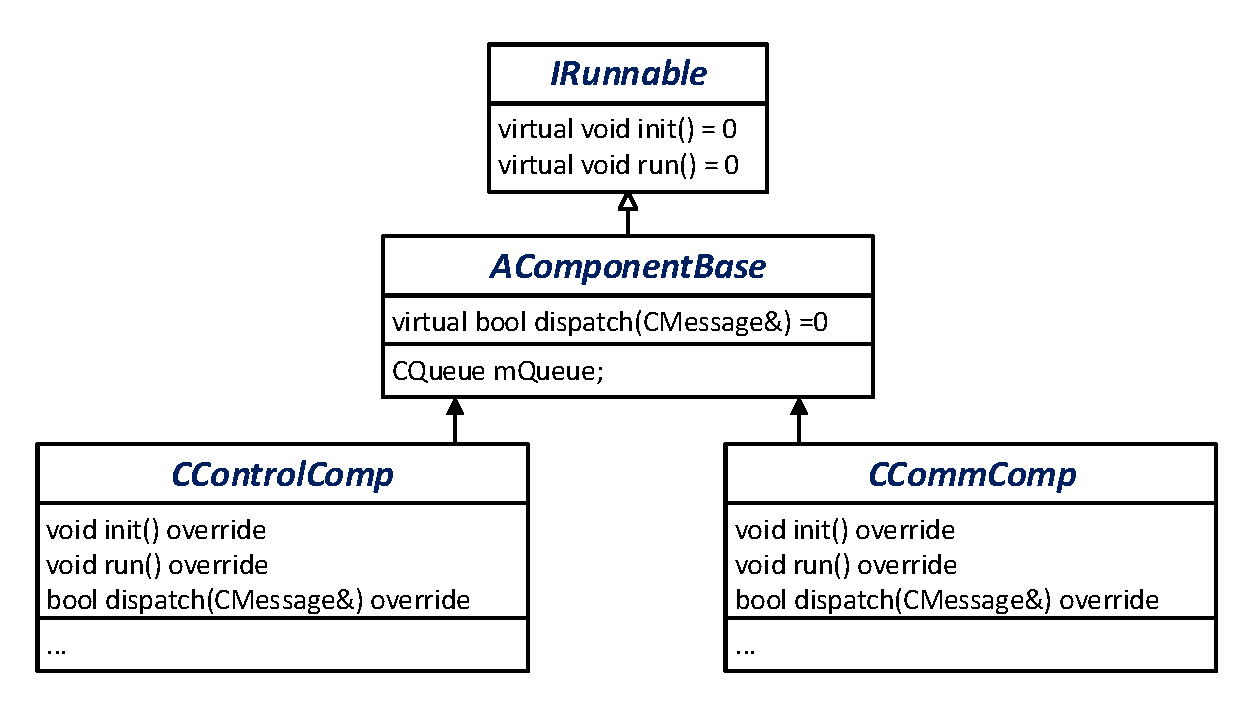
\includegraphics[width=0.6\linewidth]{img/SW_1_KA_KD.pdf}
\caption{Klassendiagramm der Komponenten}
\end{figure}

Im nächsten Schritt muss ein Weg zum Datenaustausch zwischen den Komponenten etabliert werden. Einerseits müssen Messdaten und Signale aus dem Regelkreis von der Regelungs- and die Kommunikationseinheit gesendet werden, welche diese anschließend an den Host-PC weiterleitet. Andererseits werden die Steuerbefehle des Host-PCs von der Kommunikationskomponente empfangen und an die Regelungskomponente gereicht. Da in diesem Anwendungsfall lediglich kleine Datenmengen versendet werden, werden Nachrichten für deren Austausch verwendet (\cite{Wietzke1}, S. 196). Die Nachrichten werden in Form der Klasse \textit{CMessage} implementiert, welche aus einem Datenfeld, einem Ereignis und einem Zeitstempel komponiert werden. Das Ereignis wird als Enumeration realisiert und gibt den Inhalt der Daten bzw. den jeweiligen Befehl wieder. Der Zeitstempel gibt den Abtastzeitpunkt der Signale aus dem Regelkreis wieder. 
\begin{lstlisting}[caption={Beispielhafte Implementierung der Events und Nachrichten},captionpos=b]
enum class EEvent
{
	DEFAULT_IGNORE = 0,
	TIMER_TICK     = 1,
	STATE_DATA     = 2,
	...
}
class CMessage
{
public:
	EEvent getEvent() const;
	UInt8* getDataPtr();
	...
public:

private:
	static constexpr UInt32 sDataSize = 32U;

	EEvent  mEvent;
	Float32 mTime;	
	UInt8   mData[sDataSize];
};
\end{lstlisting}
Des weiteren besitzt die Klasse \textit{CMessage}Methoden und Konstruktoren um die Datenfelder entsprechend zu füllen und auszulesen. Um die Nachrichten zu empfangen besitzen die Komponenten Eingangspuffer die als Queues implementiert werden. Die Erzeugung der Nachrichten wird von einem Proxy übernommen (\cite{Wietzke1}, S. 285 ff.), der Methoden für die unterschiedlichen Ereignisse bereitstellt. Des weiteren kennt der Proxy die Queues der Komponenten und legt neue Nachrichten, in Abhängigkeit von dem jeweiligen Event, in die Eingangspuffers des zugehörigen Empfängers.
\begin{lstlisting}[caption={Aufbau der Proxy-Klasse},captionpos=b]
class CProxy
{
	public:
		bool transmitStateVector(const StateVector& x);
		bool onTimerTick();
		bool onClientConnect();
		...
};
\end{lstlisting}
Mit Hilfe der Nachrichtenkommunikation kann auch das Ablaufschema der Komponenten verallgemeinert werden. Beim Starten der Threads werden die Komponenten zunächst über den Aufruf ihrer \textit{init()}-Methoden initialisiert, anschließend wird die \textit{run()}-Methode ausgeführt, welche in diesem Fall eine Endlosschleife darstellt. In einem Durchlauf wird geprüft ob neue Nachrichten vorhanden sind, trifft dies zu wird die Nachricht über die \textit{dispatch()}-Methode verarbeitet. Andernfalls legt sich der Thread schlafen bis neue Nachrichten zur Verfügung stehen. Hieraus ergeben sich zwei Vorteile. Einerseits werden die Komponenten nach einem einheitlichen Konzept entworfen, lediglich die Implementierung der \textit{init()}- und \textit{dispatch()}-Methode unterscheiden sich, andererseits wird durch die Synchronisation der Komponenten deren Laufzeit reduziert.
\newpage
\section{Entwurf der Regelungskomponente}
Die Aufgabe der Regelungskomponente besteht darin den Kontroll- und Signalfluss der verschiedenen Versuche zu steuern. Diese Umsetzung erfolgt mit Hilfe eines Zustandautomats, welcher die Trennung der Kontrolllogik und der auszuführenden Aktionen ermöglicht. Des weiteren kann die Applikation bei diesem Ansatz problemlos durch weitere Versuche und Anwendungsfälle erweitert werden. 
Prinzipiell lässt sich der logische Ablauf der Komponente mit einem einfachen Zustandsdiagramm modellieren. Auf der obersten Ebene existiert ein \textit{Standby}-Zustand, der die Inaktivität der Komponente widerspiegelt. Des weiteren enthält diese Ebene Zustände für die verschiedenen Versuche. Diese werden betreten, wenn die Komponente ein Event mit dem entsprechenden Befehl zur Ausführung des Versuchs erhält.
\begin{figure}[h!]
\centering
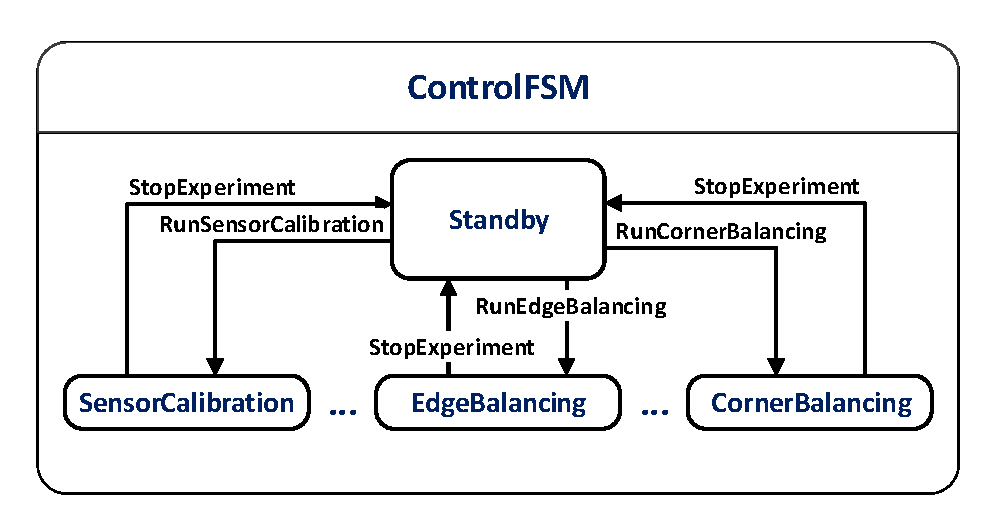
\includegraphics[width=0.7\linewidth]{img/SW_2_ControlComp_SC.pdf}
\caption{Zustandsdiagramm der Kontrol-Komponente}
\end{figure}

Ein solches Zustandsdiagramm kann z.B. mit einer objektorientierten Adaption der Methode von Samek \cite[S. 246 ff.]{Wietzke1} implementiert werden. Hierbei werden Zustände als Methoden der FSM realisiert, wobei für Oberzustände eigene Klassen entworfen werden, die wiederum Methoden für die jeweiligen Unterzustände besitzen. Die Referenzierung des aktuellen Zustandes erfolgt über einen Funktionenzeiger, der auf die Methode des entsprechenden Zustandes gerichtet ist. 

Als Basis der Typenhierachie dient die abstrakte Klasse \textit{AState}, welche den Zustandstypen als Methodenzeiger definiert, eine Standardimplementierung der \textit{dispatch()}-Methode vorgibt und statische Membervariablen deklariert um die Verarbeitung interner Events zu ermöglichen.
\begin{lstlisting}[caption={Abstrakte Basisklasse für die Zustände},captionpos=b]
class AState
{
protected:
	using StatePtr = bool (AState::*)(CMessage&);
public:
	virtual bool onInitial(CMessage& msg) = 0;
	virtual bool dispatch(CMessage& msg);
	...
protected:
	StatePtr mStatePtr;
	static constexpr StatePtr sInitial = 
			static_cast<StatePtr>(AState::onInitial);
	static CMessage sInternalQueue;
	static UInt32   sQueueSize;
};
\end{lstlisting}
Die Methode \textit{onInitial()} wird verwendet um die FSM und Oberzustände über ein \textit{Init}-Event zu initialisieren. Die \textit{dispatch()}-Methode beschränkt sich auf den Aufruf des aktuellen Zustands.

\begin{lstlisting}[caption={Defintion der \textit{dispatch()}-Methode},captionpos=b]
bool AState::dispatch(CMessage& msg)
{
	return *(this->mStatePtr)(msg);
}
\end{lstlisting} 

Die auszuführenden Aktionen, wie z.B. die Berechnung des Regelkreises, werden in der Klasse \textit{CActionHandler} gekapselt \cite[S. 225]{Wietzke1}. Dadurch erfolgt eine klare Trennung des Kontroll- und Signalflusses. Prinzipiell besitzt \textit{CActionHandler} Methoden, die jeweils beim Betreten und Verlassen der Zustände aufgerufen wird. Zusätzlich kann er um nötige Hilfsmethoden erweitert werden.
\begin{lstlisting}[caption={Beispielhafte Implementierung des Actionhandlers},captionpos=b]
class CActionHandler
{
public:
	void enterStandby();
	void exitStandby();
	void enterSensorCalibration();
	void exitSensorCalibration();
	...
	void sampleSensorCalibration();
	void sampleEdgeBalancing();
	...
private:
	CThread    mTimerThread;
	CTimerTask mTimerTask;
	
	CHardware         mHardware;
	EdgeBalancingSF   mEdgeBalancingSF;
	ConrnerBalacingSF mCornerBalacingSF;
};
\end{lstlisting}
Für die Zeitgebung wird einer separater Timer-Task \textit{CTimerTask} verwendet, der von \textit{CActionHandler} verwaltet wird. Die Timerklasse kann mittels der Methoden \textit{pause()} und \textit{resume()} pausiert bzw. gestartet werden. Während der Ausführung schläft der Timer für eine konfigurierbare Abtastzeit und erzeugt anschließend über den Proxy ein \textit{TimerTick}-Event, welches an die Regelungskomponente weitergeleitet wird.
\begin{lstlisting}[caption={Aufbau des Timer-Tasks},captionpos=b]
class CTimerTask : public IRunnable
{
public:
	void run() override
	{
		while(true)
		{
			mRunningSem.take(true);
			mRunningSem.give();
			usleep(mPeriod);
			mProxyPtr->timerTick();
		}
	}
	bool pause(bool waitForever){return mRunningSem.take(waitForever);}
	bool resume(){mRunningSem.give();}
	void setPeriod(Int32 period){mPeriod = period;};
	...
private:
	CBinarySemaphore mRunningSem;
	Int32            mPeriod;
	CProxy*          mProxyPtr;
};
\end{lstlisting}
Der Ansatz nach Samek bringt bei diesen Anwendungsfall einen Nachteil mit sich. Für die meisten Versuche genügt eine simple Kontrolllogik, weshalb diese als einfacher Unterzustand realisiert werden. Das hat eine flache Zustandshierarchie zur Folge, die der Anzahl von Versuchen entsprechend breit ist. In der Implementierung resultiert hieraus eine umfangreiche Klasse \textit{CFSM}, da diese für jeden Unterzustand um eine Methode erweitert wird. Ebenso nimmt der Umfang der Klasse \textit{CActionHandler} mit der Anzahl der Versuche kontinuierlich zu. Dieses Problem kann zwar durch die Aufteilung in mehrere Actionhandler vermieden werden, allerdings wird dadurch die Komplexität von \textit{CFSM} weiter erhöht. Diese Problematik wird dadurch verschärft, dass es sich bei der Zustandsmaschine um den Kern der Anwendung und somit kritischen Abschnitt der Anwendung handelt. Die zu Grunde liegende Komponentenarchitektur wird zu Projektbeginn erstellt und danach kaum manipuliert. Im Gegensatz dazu wird die Zustandmaschine während des Projektsverlaufes ständig verändert und erweitert, weshalb eine unübersichtliche Implementierung besonders negativ auffällt. Aus diesem Grund wird im nächsten Schritt eine alternative Vorgehensweise vorgestellt, die sich die spezielle Struktur des Zustandsdiagrammes zu Nutze macht um eine effiziente Implementierung zu schaffen.

Zunächst sei angemerkt, dass es nicht möglich ist direkt zwischen zwei Versuchszuständen zu wechseln. Ein Versuchszustand kann nur aus dem Zustand \textit{Standby} betreten werden. Des weiteren wird nach dem Verlassen eines Versuchszustandes immer in \textit{Standby} gewechselt. Dadurch kann die Kontrolllogik der Zustandsmaschine verallgemeinert werden. Ist der momentane Unterzustand nicht \textit{Standby} und es trifft ein \textit{StopExperiment}-Event ein, so wird der Zustand verlassen und in \textit{Standby} gewechselt. Befindet sich die FSM in \textit{Standby} wird bei Eintreffen eines Events geprüft ob ein Zustandswechsel erfolgen muss. Diese Prüfung kann an die Zustände abgegeben werden. Somit stellt die Zustandsmaschine in diesem Fall lediglich eine Anfrage an alle Versuchszustände ob diese betreten werden möchten.

Die Implementierung der Zustandsmaschine setzt sich folglich aus einem \textit{Standby}-Zustand und einer Liste von Versuchszuständen zusammen. Um eine übersichtliche Codestruktur zu erhalten werden diese als Klassen entworfen, die von der abstrakten Basisklasse \textit{AState} erben.
\begin{lstlisting}[caption={Angepasste Implementierung der abstrakten Zustandsklasse},captionpos=b]
class AState
{
public:
	virtual bool dispatch(CMessage&) = 0;
	virtual bool tryEntry(CMessage&, AState*&) = 0;
	virtual void onEntry() = 0;
	virtual void onExit()  = 0;
private:
	static CMessage sInternalQueue;
	static UInt32   sQueueSize;
};
\end{lstlisting}
Die Methode \textit{dispatch()} dient zur Verteilung von eintreffenden Nachrichten. Mit Hilfe von \textit{tryEntry()} kann die Zustandmaschine prüfen ob der Zustand, in Abhängigkeit des Events, betreten werden möchte. Der folgende Ausschnitt zeigt eine mögliche Implementierung für den Zustand \textit{SensorCalibration}.
\begin{lstlisting}[caption={Beispielhafte Definition der Methode \textit{tryEntry()}},captionpos=b]
bool CSensorCalibration::tryEntry(CMessage& msg, AState*& statePtr)
{
	EEvent event = msg.getEvent();
	if(EEvent::RUN_SENSORCALIBRATION == event)
	{
		statePtr = this;
		return true;
	}
	return false;
}
\end{lstlisting}
Das zweite Argument ist eine Zeigerreferenz auf den Zustandszeiger der FSM. Falls ein Zustand betreten werden soll überschreibt er die Referenz mit seinem this-Zeiger und gibt \textit{true} zurück um den Konsum des Events zu signalisieren. Die Methoden \textit{onEntry()} und \textit{onExit()} werden zum Betreten bzw. Verlassen des Zustandes verwendet. Um auch die auszuführenden Aktionen zu trennen, wird für jede Zustandsklasse ein Actionhandler implementiert. Diese erben von der Klasse \textit{CActionBase}, die gemeinsame Ressourcen als statische Membervariablen deklariert. Ein Beispiel wären hierfür Instanzen der Klassen \textit{CHardware} oder \textit{CTimerTask}.

Um die Zustandsklassen zu einer Liste zusammenzufassen wird wieder eine lineare Typenhierarchie verwendet. Hierfür muss zunächst ein Trägerobjekt \textit{TStateHolder} entworfen werden. 
\begin{lstlisting}[caption={Implementierung der Trägerklasse für Zustände},captionpos=b]
template<class State, class Base>
class TStateHolder : public Base
{
	bool tryEntry(CMessage& msg, AState*& statePtr)
	{
		bool consumed = mState.tryEntry(msg, statePtr);
		if(consumed == false)
		{
			return Base::tryEntry(msg, statePtr);
		}
		return consumed;
	}
private:
	State mState;
};
template<class State>
class TStateHolder<State, CNullType> : public CNullType
{
public:
	bool tryEntry(CMessage& msg, AState*& statePtr)
	{
		return mState.tryEntry(msg, statePtr);
	}
private:
	State mState;
};
\end{lstlisting}
Analog zu \textit{TActionHolder} wird mittels einer Templatespezialisierung unterschieden ob das Ende der Typenliste erreicht ist. Ist dies nicht der Fall wird zunächst geprüft ob der getragene Zustand betreten werden soll. Trifft dies nicht zu wird  die \textit{tryEntry()}-Methode des nächsten Elements in der Hierarchie aufgerufen. Ein Unterschied zu \textit{TActionHolder} ist, dass eine Komposition aus dem Zustandsobjekt verwendet wird. Dadurch werden die Methoden des Zustandes geschützt. Die FSM kann lediglich auf den, über ihren Zustandszeiger referenzierten, Zustand zugreifen.
Die Implementierung der Zustandsmaschine basiert ebenfalls auf einem Template, welchem die Typenliste der Versuchszustände übergeben wird. Des weiteren erbt die Templateklasse von \textit{AState} um Zugriff auf die interne Queue zu erhalten.
\begin{lstlisting}[caption={Implementierung der Templateklasse für die Zustandsmaschine},captionpos=b]
template<class StateList>
class TFSM : public AState
{
public:
	bool dispatch(CMessage& msg) override;
	bool tryEntry(CMessage& msg, AState*& statePtr) override;
	void onEntry() override;
	void onExit() override;
	bool onStandby(CMessage& msg);
	void handleUnconsumedEvent(CMessage& msg);
private:
	AState*                mStatePtr;
	TLinHierach<StateList> mStateList;
	CAction                mAction;
};
\end{lstlisting}
Neben dem Interface von \textit{AState} besitzt die Klasse zwei weitere Methoden. Wobei die erste den Zustand \textit{Standby} repräsentiert. Die zweite Methode wird genutzt um nicht konsumierte Events, was für gewöhnlich einem Fehlverhalten der FSM entspricht, abfängt. Zunächst wird die \textit{dispatch()}-Methode betrachtet. Zu Beginn wird der aktuelle Unterzustand aufgerufen. Falls das Ereignis nicht konsumiert wird und es sich um \textit{StopExperiment} handelt, wird der aktuelle Unterzustand verlassen und in \textit{Standby gewechselt}. Zuletzt wird die interne Queue abgearbeitet.
\begin{lstlisting}[caption={Definition der Methode \textit{dispatch()}},captionpos=b]
template<class StateList>
bool TFSM<StateList>::dispatch(CMessage& msg)
{
	bool consumed = false;
	if(mStatePtr == nullptr)
	{
		consumed = this->onStandby(msg);
	}
	else
	{
		consumed = mStatePtr->dispatch(msg);
	}
	
	if(consumed == false)
	{
		EEvent event = msg.getEvent();
		if(EEvent::StopExperiment == event)
		{
			mStatePtr->onExit();
			mStatePtr = nullptr;
			mAction.entryStandby();
		}
	}
	
	while(squeueSize > 0U)
	{
		CMessage internalMsg(sInternalQueue);
		sQueueSize = 0U;
		consumed = mStatePtr->dispatch(internalMsg);
	}
	return consumed;
}
\end{lstlisting}
Im Zustand \textit{Standby} wird das Ereignis an alle Unterzustände übergeben um zu prüfen, ob diese betreten werden sollen. 
\begin{lstlisting}[caption={Implementierung der Methode \textit{onStandby()}},captionpos=b]
template<class StateList>
bool TFSM<StateList>::onStandby(CMessage& msg)
{
	bool consumed = this->tryEntry(msg);
	if(consumed == true)
	{
		mAction.exitStandby();
		mStatePtr->onEntry();
	}
	return consumed;
}
\end{lstlisting}
Die Methode \textit{tryEntry()} stößt lediglich die Abfrage der Unterzustände an.
\begin{lstlisting}[caption={Implementierung der Methode \textit{tryEntry()}},captionpos=b]
template<class StateList>
bool TFSM<StateList>::tryEntry(CMessage& msg, AState*& statePtr)
{
	return mStateList.tryEntry(mg, statePtr);
}
\end{lstlisting}
Die Vorteile dieses Konzept verdeutlichen sich wieder bei der Anwendung. Für jeden Versuch wird eine Zustandsklasse und Actionhandler entworfen, wodurch eine übersichtliche Projektstruktur entsteht. Um die letztendliche Zustandsmachine zu erhalten wird lediglich \textit{TFSM} mit der gewünschten Liste von Zustandstypen instantiiert.
\begin{lstlisting}[caption={Beispielhafte Instantiierung der Zustandsmaschine},captionpos=b]
using StateList  = TYPELIST_4(CSensorCalib, CADCCalib, 
                              CEdgeBalance, CCornerBalance);
using ControlFSM = TFSM<StateList>;
ControlFSM myFSM;
\end{lstlisting}
Sollen weitere Zustände hinzugefügt oder entfernt werden muss lediglich die Typdefinition von \textit{StateList} angepasst werden. Um Coderedundanzen zu vermeiden kann für die Unterzustände auch eine Templateklasse entworfen werden, die das Eintrittsereignis und den Actionhandler als Parameter entgegennimmt. 
\begin{lstlisting}[caption={Templateklasse für einfache Versuchszustände},captionpos=b]
/* TSubState.h */
template<const EEvent entryEvent, class Action>
class TSubState : public AState
{
public:
	bool tryEntry(CMessage& msg, AState*& statePtr) override
	{
		if(entryEvent == msg.getEvent())
		{
			statePtr = this;
			return true;
		}
		return false;
	};
	bool dispatch(CMessage& msg) override;
	void onEntry() override;
	void onExit() override;
private:
	Action mAction;
};
\end{lstlisting}
Die Unterzustände spezialisieren dann lediglich die Methoden \textit{dispatch()}, \textit{onEntry()} und \textit{onExit()}, wie das folgende Beispiel zeigt.
\begin{lstlisting}[caption={Beispielhafte Instantiierung des Versuchstemplate},captionpos=b]
/* CADCCalib.cpp */
using CADCCalib = TSubState<EEvent::RunADCCalib, CADCCalibAction>;
template<>
bool CADCCalib::dispatch(CMessage& msg)
{
	EEvent event = msg.getEvent();
	if(EEvent::TIMERTICK == event)
	{
		mAction.sampleADCCalib();
		return true;
	}
	...
	return false;
}
template<>
void CADCCalib::onEntry()
{
	cout << "Entering ADC-Calibration . . . " << endl;
	mAction.resumeTimer();
}
template<>
void CADCCalib::onExit()
{
	cout << "Exiting ADC-Calibration . . . " << endl;
	mAction.pauseTimer();
}
\end{lstlisting}

\ifx\FORMAT\undefined
\end{document}
\fi

\documentclass[11pt]{book}
\usepackage{amsmath,mathtools}
\usepackage[utf8]{inputenc}
\usepackage[ngerman]{babel}
\usepackage{acronym}
\usepackage{graphicx} 
\usepackage{epstopdf}
\usepackage{svg}
\usepackage{multirow}
\usepackage{amssymb}
\usepackage{trfsigns}
\usepackage{setspace}
\usepackage{yfonts}

\onehalfspacing


%Hyperlinks package, links aus inhaltsverzeichnis
\usepackage{hyperref}
\hypersetup{
    colorlinks=false, %set true if you want colored links
    linktoc=all
}
%Blattformatierung
\usepackage{geometry}
\geometry{a4paper, top=25mm, left=30mm, right=25mm, bottom=20mm}

%Listing
\usepackage{courier}
\usepackage{listings}
\usepackage{color}
 \lstset{
   frame=tb,
   framexleftmargin=2.5em,
   basicstyle=\small\linespread{0.9}\bfseries\ttfamily,
   emph={square}, 
   emphstyle=\color{blue}\texttt,
   emph={[2]root,base},
   emphstyle={[2]\color{yac}\texttt},
   showstringspaces=false,
   flexiblecolumns=false,
   tabsize=2,
   numbers=left,
   numberstyle=\small\bfseries\ttfamily,
   numberblanklines=false,
   stepnumber=1,
   numbersep=10pt,
   xleftmargin=25pt
 }

\begin{document}

\def\presuper#1#2%
	{\mathop{}%
	\mathopen{\vphantom{#2}}^{#1}%
	\kern-\scriptspace%
	#2}
%Display vecotr in a reference frame
\newcommand{\vecBS}[4]{\presuper{#1}{\begin{pmatrix}
#2 \\ #3 \\ #4
\end{pmatrix}}}
%Boldsymbol shortcut
\newcommand{\bs}[1]{\boldsymbol{#1}}
%Bezugssystemdefinition
\newcommand{\defBS}[1]{\{#1\} [ \bs{e}_{{#1}_1},\bs{e}_{{#1}_2}, \bs{e}_{{#1}_3} ]}
%Projektionsmatrix
\newcommand{\pMat}[2]{\presuper{#1}{\bs{P}}^{#2}}
%Differenation in Respekt zu BS
\newcommand{\diffIn}[3]{\frac{\presuper{#1}{d{#2}}}{d#3}}
\newcommand{\partialDiffIn}[3]{\frac{\presuper{#1}{\partial{#2}}}{\partial #3}}
%Geschwindigkeit/Beschleunigung
\newcommand{\vel}[3]{\presuper{#1}{\bs{#2}}^{#3}}

%Rightarrow with spaceing
\newcommand{\rArrow}{\hspace{5pt}\rightarrow\hspace{5pt}}
%Inneres Produkt
\newcommand{\inProd}[2]{\langle {#1}, {#2} \rangle}

%System macro
\newcommand{\cSS}[3]{\textfrak{S}($\bs{#1}$,$\bs{#2}$,$\bs{#3}$)}
\newcommand{\dSS}[3]{\textfrak{D}($\bs{#1}$,$\bs{#2}$,$\bs{#3}$)}

%Laplace transform sign with spaces
\newcommand{\myLaplace}{\hspace{15pt}\laplace\hspace{15pt}}

\newcommand*{\signed}[1]{%
        \nolinebreak[3]\hspace*{\fill}\mbox{\emph{#1}}
    }

\chapter{Modellbildung Würfel auf Ecke}
Das nächste Ziel besteht darin ein Regelungskonzept zu entwickeln, welches das Balancieren des Würfels auf einer Ecke ermöglicht. Hierfür werden drei Motor verwendet, wodurch das gesamte System über sechs Freiheitsgrade verfügt. Die Vorgehensweise erfolgt analog zu dem Reglerentwurf der Würfelseite. Somit besteht der erste Schritt in dem Entwurf eines mechanischen Modells, welches wiederum zu einer Zustandsraumdarstellung führt, die als Grundlage für den Reglerentwurf verwendet wird.
Zu Beginn dieses Kapitels werden die Systemparameter vorgestellt, deren Bestimmung diskutiert und erste Annahmen getroffen um die weitere Modellbildung zu vereinfachen. Im zweiten Abschnitt wird die Kinematik des Systems untersucht. Hierbei werden zunächst die nötigen Bezugssysteme und generalisierten Koordinaten definiert, die anschließend für die Bestimmung der generalisierten und partiellen Geschwindigkeiten benötigt werden.
Der nächste Abschnitt widmet sich der Kinematik. Hierunter fallen sowohl die wirkenden Kräfte und die draus resultierenden Drehmomente als auch die Trägheitsmomente der Körper. Daraus werden die generalisierten Kräfte und Trägheitskräfte ermittelt, welche nach Kanes Gleichungen auf die Bewegungsgleichungen führen. Diese werden anschließend in eine Zustandsraumdarstellung überführt.

\section{Systemparameter}\label{TM_3D_Systemparameter}
Zunächst werden die Parameter des mechanischen Systems vorgestellt. Das System setzt sich aus drei Schwungmassen und dem Würfelkörper zusammen. Unter dem Würfelkörper ist das Würfelgehäuse inklusive der montierten Motoren, Sensoren und Elektrik zu verstehen und wird mit $K$ bezeichnet. Bei der Herleitung der Bewegungsgleichungen wird die Annahme getroffen, dass der Würfelkörper nicht translativ bewegt wird, sondern lediglich um Punkt $O$ rotiert. Der Punkt $O$ ist hierbei die Ecke auf welcher der Würfel balanciert. Des weiteren beschreiben alle Ortsvektoren den Vektor von $O$ zu dem jeweiligen Zielpunkt. Die drei Schwungmassen $R_i$ sind mit jeweils einem rotatorischem Freiheitsgrad auf den Motorwellen gelagert. Die Position der Lagerung wird mit $M_i$ bezeichnet und fällt auf Grund des symmetrischen Aufbau der Schwungmassen mit deren Schwerpunkt zusammen.
Die Massen
\begin{equation}
m_R = 0{,}155\text{ kg}
\end{equation}
und Trägheitstensoren $\bs{I}^{Ri/Mi}$ der Schwungmassen werden mit Hilfe der CAD-Anwendung ermittelt. 
Die Trägheitstensoren werden dabei aus der Perspektive des körperfesten Bezugssystem $K$ relativ zu den Punkten $M_i$ bestimmt. Für den Trägheitstensor der Schwungmasse $R_1$ ergibt sich der Wert
\begin{equation}
 \bs{I}^{R1/M1} = \begin{bmatrix}
3.358\cdot 10^{-4} & 2{,}641\cdot 10^{-11} & 0 
\\
2{,}651\cdot 10^{-11} & 1{,}961\cdot 10^{-4} & 4{,}527\cdot 10^{-9} 
\\
0 & 4.527\cdot 10^{-9} & 1{,}691\cdot 10^{-4}
\end{bmatrix} \text{ kg}\cdot \text{m}^2 \,.
\end{equation}
Hieran ist zu erkennen, dass die Vektorbasis des Bezugssystem $K$ nahezu den Haupträgheitsachsen der Schwungmasse entspricht, da die Devitationsmomente um die Größenordnung $10^{5}$ kleiner als die Haupträgheitsmomente sind. Deshalb wird bei der  
folgenden Untersuchung die Annahme getroffen, dass die Devitationsmomente vernachlässigt werden können und es gilt 
\begin{equation}
\begin{split}
\bs{I}^{R1/M1} &\equiv \begin{bmatrix}
I^{R1}_{11} & 0 & 0 \\ 0 & I^{R1}_{22} & 0 \\ 0 & 0 & I^{R1}_{33}
\end{bmatrix} = 
\begin{bmatrix}
3.358\cdot 10^{-4} & 0 & 0 \\
0 & 1{,}961\cdot 10^{-4} & 0 \\
0 & 0 & 1{,}691\cdot 10^{-4}
\end{bmatrix} \text{ kg}\cdot \text{m}^2
\\
\bs{I}^{R2/M2} &\equiv \begin{bmatrix}
I^{R2}_{11} & 0 & 0 \\ 0 & I^{R2}_{22} & 0 \\ 0 & 0 & I^{R2}_{33}
\end{bmatrix} = 
\begin{bmatrix}
1{,}691\cdot 10^{-4} & 0 & 0 \\
0 & 3.358\cdot 10^{-4} & 0 \\
0 & 0 & 1{,}961\cdot 10^{-4}
\end{bmatrix} \text{ kg}\cdot \text{m}^2
\\
\bs{I}^{R3/M3} &\equiv \begin{bmatrix}
I^{R3}_{11} & 0 & 0 \\ 0 & I^{R3}_{22} & 0 \\ 0 & 0 & I^{R3}_{33}
\end{bmatrix} = 
\begin{bmatrix}
1{,}961\cdot 10^{-4} & 0 & 0 \\
0 & 1{,}691\cdot 10^{-4} & 0 \\
0 & 0 & 3.358\cdot 10^{-4}
\end{bmatrix} \text{ kg}\cdot \text{m}^2 \,.
\end{split}
\end{equation}
Für die Masse des Würfelkörpers $m_K$ und des Gesamtsystems $m$ ergibt sich
\begin{equation}
m_K = 1{,}07 \text{ kg} \hspace{35pt} m = m_K + 3\cdot m_R = 1{,}532 \text{ kg}\,.
\end{equation}
Bei der Berechnung des Trägheittensors $\bs{I}^{GH/0}$ des Würfelkörpers um den Punkt $O$ wird der Einfluss der Schwungmassen nicht beachtet. Dies erfolgt bei der Berechnung der Trägheitsmomente in den folgenden Abschnitten. Somit ergibt sich für den Trägheitstensor
\begin{equation}
\begin{split}
\bs{I}^{GH/O} &= \begin{bmatrix}
I^{GH}_{11} & I^{GH}_{12} & I^{GH}_{13} \\
I^{GH}_{21} & I^{GH}_{22} & I^{GH}_{23} \\
I^{GH}_{31} & I^{GH}_{32} & I^{GH}_{33}
\end{bmatrix} \\
&=
\begin{bmatrix}
1{,}520\cdot 10^{-2} & -5{,}201\cdot 10^{-3} & 5{,}375\cdot 10^{-3} \\
-5{,}201\cdot 10^{-3} & 1{,}52\cdot 10^{-2} & 5{,}225\cdot 10^{-3} \\
5{,}375\cdot 10^{-3} & 5{,}225\cdot 10^{-3} & 1{,}542\cdot 10^{-2}
\end{bmatrix}\text{ kg}\cdot \text{m}^2 \,.
\end{split}
\end{equation}
Der Ortsvektor $\bs{c}$ des Schwerpunkt des Gesamtsystems wird ebenfalls numerisch ermittelt. Da sich die Komponenten des Ortsvektors $\bs{c}$ lediglich um $10^{-1}\text{mm}$ unterscheiden werden diese als identischen angenommen.
\begin{equation}
\bs{c} = \vecBS{K}{-6,61}{-6,60}{-6,57}\text{ cm} \approx \vecBS{K}{l_C}{l_C}{l_C} \hspace{15pt} \vert \hspace{15pt} l_C = 6,6\text{ cm}
\end{equation}
Des weiteren entsteht durch die Bewegung der Schwungmassen ein Reibmoment,welches als proportional zu den Winkelgeschwindigkeiten der Schwungmassen modelliert wird. Für Proportionalitätsfaktor $C_{\psi}$ wurde experimentell der  Wert 
\begin{equation}
C_{\psi} = 3,1176\cdot 10^{-5}\text{ kg}\cdot \text{m}^2 \cdot \text{s}^{-1}
\end{equation}
ermittelt.

\section{Untersuchung der Kinematik}
Der erste Schritt in der Modellbildung besteht in der Definition der Bezugssysteme, welche zur Beschreibung der Systembewegung dienen. Der Ausgangspunkt ist das Inertialsystem $A$, welches durch die drei Einheitsvektoren $\bs{a}\idx1$, $\bs{a}\idx2$ und $\bs{a}\idx3$ definiert wird. Das Würfelgehäuse verfügt über drei rotatorische Freiheitsgrade, welche durch die Winkel $\varphi\idx1$, $\varphi\idx2$ und $\varphi\idx3$ beschrieben werden. 
\begin{figure}[!h]
\centering
\includegraphics[width=0.75\textwidth]{img/tm_corner_drawing.eps}
\caption{Mechanische Skizze des Würfels}
\end{figure}
Durch die Rotation des Würfels um den Winkel $\varphi\idx1$ in Richtung des Vektors $\bs{a}\idx1$ entsteht das Hilfsbezugssystem $B$, welches durch die Einheitsvektoren $\bs{b}\idx1$, $\bs{b}\idx2$ und $\bs{b}\idx3$ definiert wird. Für die Abbildungsmatrix gilt
\begin{equation}
\pMat{A}{B} = \begin{bmatrix}
1 & 0 & 0 \\ 0 & c_{\varphi\idx1} & s_{\varphi\idx1} \\ 0 & -s_{\varphi\idx1} & c_{\varphi\idx1}
\end{bmatrix} \,.
\end{equation}
Die Rotation um den Winkel $\varphi\idx2$ in Richtung des Vektors $\bs{b}\idx2$ führt zu dem zweiten Hilfsbezugssystem $C$ mit den drei Einheitsvektoren $\bs{c}\idx1$, $\bs{c}\idx2$ und $\bs{c}\idx3$ und der Projektionsmatrix
\begin{equation}
\pMat{B}{C} = \begin{bmatrix}
c_{\varphi\idx2} & 0 & -s_{\varphi\idx2} \\
0 & 1 & 0 \\
 s_{\varphi\idx2} & 0 & c_{\varphi\idx2}
\end{bmatrix} \,.
\end{equation}
Die letzte Rotation des Würfels in Richtung von $\bs{c}\idx3$ um den Winkel $\varphi\idx3$ führt zu dem körperfesten Bezugssystem $K$, welches durch die drei Vektoren $\bs{k}\idx1$, $\bs{k}\idx2$ und $\bs{k}\idx3$ definiert ist. Für die Abbildungsmatrix gilt 
\begin{equation}
\pMat{C}{K} = \begin{bmatrix}
c_{\varphi\idx3} & s_{\varphi\idx3} & 0 \\ -s_{\varphi\idx3} & c_{\varphi\idx3} & 0 \\ 0 & 0 & 1
\end{bmatrix} \,.
\end{equation}
Hier sei angemerkt, dass es sich bei den Bezugssystemen $B$ und $C$ um theoretische Konstrukte handelt, für die kein physisches Gegenstück existiert. Sie werden lediglich als Hilfsmittel zur Beschreibung des Systems verwendet (\cite{KaneBook}, S. 24 ff.).

Durch die Rotation der Schwungmassen besitzt das System drei weitere Freiheitsgrade, welche von den Winkeln $\psi\idx1$, $\psi\idx2$ und $\psi\idx3$ beschrieben werden. Somit entstehen drei weitere Bezugssysteme, deren Vektorbasen jeweils an den Schwungmassen fixiert sind. Allerdings spielen diese keine weitere Rolle, da es sich bei den Winkeln $\psi_i$ um zyklische Koordinaten handelt. Das heißt, dass der Impuls des Systems nicht von der Ausrichtung der Schwungmassen beeinflusst wird. Lediglich die Winkelgeschwindigkeiten $\dot{\psi}_i$ wirken auf Grund der Reibung auf das System.

Die Position und Ausrichtung des Systems wird von den sechs Winkeln $\varphi_i$ und $\psi_i$ vollständig beschrieben. Deshalb werden diese als generalisierte Koordinaten 
\begin{equation}
q_i \equiv \varphi_i \hspace{35pt} q_j \equiv \psi_i \hspace{35pt} (i=1,2,3, j=4,5,6) \,.
\end{equation}
Mit Hilfe der Bezugssysteme und generalisierten Koordinaten können nun die Winkelgeschwindigkeit des Würfels $\vel{A}{\omega}{K}$ und der Schwungmassen $\vel{A}{\omega}{R_i}$ bestimmt werden. Diese ergeben sich aus der Addition der relativen Rotationsgeschwindigkeiten der Bezugssysteme zueinander (\cite{KaneBook}, S. 24).
\begin{equation}
\begin{split}
\vel{A}{\omega}{K} &= \vel{A}{\omega}{B}+\vel{B}{\omega}{C}+\vel{C}{\omega}{K} = \vecBS{A}{\dot{\varphi}\idx1}{0}{0} + \vecBS{B}{0}{\dot{\varphi}\idx2}{0} + \vecBS{C}{0}{0}{\dot{\varphi}\idx3} \\
&= \vecBS{K}
{\dot{\varphi}\idx2\cdot s_{\varphi\idx3} + \dot{\varphi}\idx1 \cdot c_{\varphi\idx2}\cdot c_{\varphi\idx3}}
{\dot{\varphi}\idx2\cdot c_{\varphi\idx3} - \dot{\varphi}\idx1 \cdot c_{\varphi\idx2}\cdot s_{\varphi\idx3}}
{\dot{\varphi}\idx3 + \dot{\varphi}\idx1\cdot s_{\varphi\idx2}}
\end{split}
\end{equation}
Die Winkelgeschwindigkeiten der Schwungmassen $\vel{K}{\omega}{R_i}$ relativ zu dem Würfel entsprechen der ersten Ableitung der Winkel $\psi_i$. Mit Hilfe des Additionstheorems für Winkelgeschwindigkeiten kann daraus auch die absolute Winkelgeschwindigkeit der Schwungmassen 
\begin{equation}
\vel{K}{\omega}{R_1} = \vecBS{K}{\dot{\psi}\idx1}{0}{0} \hspace{35pt}
\vel{K}{\omega}{R_2} = \vecBS{K}{0}{\dot{\psi}\idx2}{0} \hspace{35pt}
\vel{K}{\omega}{R_3} = \vecBS{K}{0}{0}{\dot{\psi}\idx3} 
\end{equation}
\begin{equation}
\vel{A}{\omega}{R_i} = \vel{A}{\omega}{K} + \vel{K}{\omega}{R_i} \hspace{35pt} (i=1,2,3)
\end{equation}
berechnet werden. Im nächsten Schritt werden die absoluten Geschwindigkeiten der Teilsysteme in Komponenten zerlegt, welche sich aus den generalisierten Geschwindigkeiten $u_i$ und partiellen Geschwindigkeiten $\vel{A}{\omega}{j}_i$ zusammensetzen. Hierfür müssen zu nächst die generalisierten Geschwindigkeiten $u_i$ definiert werden. An dieser Stelle sei erwähnt, dass die Definition der generalisierten Geschwindigkeiten die Form der resultierenden Bewegungsgleichungen stark beeinflusst. Das letztendliche Ziel bei der Wahl der generalisierten Geschwindigkeiten ist es möglichst einfache Bewegungsgleichungen zu erhalten. Dies wird erreicht , in dem die generalisierten Geschwindigkeiten so gewählt werden, dass die Geschwindigkeiten der Körper im Intertialsystem auf möglichst einfache Terme reduziert werden (\cite{KanePaper}). Nach diesem Ansatz werden die  generalisierten Geschwindigkeiten 
\begin{equation}
\begin{split}
u\idx1 &= \dot{\varphi}\idx2\cdot s_{\varphi\idx3} + \dot{\varphi}\idx1\cdot c_{\varphi\idx2}\cdot c_{\varphi\idx3} \\
u\idx2 &= \dot{\varphi}\idx2\cdot c_{\varphi\idx3} - \dot{\varphi}\idx1\cdot c_{\varphi\idx2}\cdot s_{\varphi\idx3} \\
u\idx3 &= \dot{\varphi}\idx3 + \dot{\varphi}\idx1\cdot s_{\varphi\idx2} \\
u_4 &= \dot{\varphi}\idx2\cdot s_{\varphi\idx3} + \dot{\varphi}\idx1\cdot c_{\varphi\idx2}\cdot c_{\varphi\idx3} + \dot{\psi}\idx1 \\
u_5 &= \dot{\varphi}\idx2\cdot c_{\varphi\idx3} - \dot{\varphi}\idx1\cdot c_{\varphi\idx2}\cdot s_{\varphi\idx3} + \dot{\psi}\idx2 \\
u_6 &= \dot{\varphi}\idx3 + \dot{\varphi}\idx1\cdot s_{\varphi\idx2} + \dot{\psi}\idx3
\end{split}
\end{equation}
gewählt. Mit diesen Definitionen können die Winkelgeschwindigkeiten der Körper im A in die Form 
\begin{equation}
\vel{A}{\omega}{K} = \vecBS{K}{u\idx1}{u\idx2}{u\idx3}, \vel{A}{\omega}{R1} = \vecBS{K}{u\idx4}{u\idx2}{u\idx3}, \vel{A}{\omega}{R2} = \vecBS{K}{u\idx1}{u\idx5}{u\idx3}, \vel{A}{\omega}{R3} = \vecBS{K}{u\idx1}{u\idx2}{u\idx6}
\end{equation}
gebracht werden. Die Einführung der generalisierten Geschwindigkeiten führt einerseits zu einem einfachen  Ausdruck der absoluten Winkelgeschwindigkeiten aus Perspektive des körperfesten Bezugssystem $K$. Andererseits können dadurch auch die partiellen Geschwindigkeiten $\vel{A}{\omega}{j}_i$ in einfachen Termen ausgedrückt werden. Für diese gilt 
\begin{align}
\vel{A}{\omega}{K} &= u\idx1 \cdot \bs{k}\idx1 + u\idx2 \cdot \bs{k}\idx2 + u\idx3 \cdot \bs{k}\idx3 &\rArrow &\vel{A}{\omega}{K}\idx1 = \bs{k}\idx1, \vel{A}{\omega}{K}\idx2 = \bs{k}\idx2, \vel{A}{\omega}{K}\idx3 = \bs{k}\idx3 \\
& & &\vel{A}{\omega}{K}\idx4 = 0, \vel{A}{\omega}{K}\idx5 = 0, \vel{A}{\omega}{K}\idx6 = 0 \nonumber
\\
\vel{A}{\omega}{R\idx1} &= u\idx4 \cdot \bs{k}\idx1 + u\idx2 \cdot \bs{k}\idx2 + u\idx3 \cdot \bs{k}\idx3 &\rArrow 
&\vel{A}{\omega}{K}\idx1 = 0, \vel{A}{\omega}{K}\idx2 = \bs{k}\idx2, \vel{A}{\omega}{K}\idx3 = \bs{k}\idx3 \\
& & &\vel{A}{\omega}{K}\idx4 = \bs{k}\idx1, \vel{A}{\omega}{K}\idx5 = 0, \vel{A}{\omega}{K}\idx6 = 0 \nonumber
\\
\vel{A}{\omega}{R\idx2} &= u\idx1 \cdot \bs{k}\idx1 + u\idx5 \cdot \bs{k}\idx2 + u\idx3 \cdot \bs{k}\idx3&\rArrow 
&\vel{A}{\omega}{K}\idx1 = \bs{k}\idx1, \vel{A}{\omega}{K}\idx2 = 0, \vel{A}{\omega}{K}\idx3 = \bs{k}\idx3 \\
& & &\vel{A}{\omega}{K}\idx4 = 0, \vel{A}{\omega}{K}\idx5 = \bs{k}\idx2, \vel{A}{\omega}{K}\idx6 = 0 \nonumber
\\
\vel{A}{\omega}{R\idx3} &= u\idx1 \cdot \bs{k}\idx1 + u\idx2 \cdot \bs{k}\idx2 + u\idx6 \cdot \bs{k}\idx3&\rArrow 
&\vel{A}{\omega}{K}\idx1 = \bs{k}\idx1, \vel{A}{\omega}{K}\idx2 = \bs{k}\idx2, \vel{A}{\omega}{K}\idx3 = 0 \\
& & &\vel{A}{\omega}{K}\idx4 = 0, \vel{A}{\omega}{K}\idx5 = 0, \vel{A}{\omega}{K}\idx6 = \bs{k}\idx3 \nonumber \,
\end{align}
Die Beudeutung der generalisierten und partiellen Geschwindigkeiten kann so interpretiert werden, dass sie eine Unterteilung der Bewegung in Betrag und Richtung darstellen. Die generalisierten Geschwindigkeiten geben als skalare Größen den Betrag der Geschwindigkeit wieder, wobei die entsprechenden partiellen Geschwindigkeiten die Bewegungsrichtung darstellen.


\section{Untersuchung der Kinetik}
Der nächste Schritt besteht darin die Kräfte zu modellieren, welche auf den Würfelkörper und die drei Schwungmassen wirken. Aus diesen können im Anschluss mit Hilfe der partiellen Geschwindigkeiten die generalisierten aktiven Kräfte $F_i$ ermittelt werden.
Zunächst sollen die resultierenden Drehmomente $\bs{T}^{Ri/Mi}$ der Schwungmassen $R_i$ um ihren jeweiligen Drehpunkt $M_i$ bestimmt werden. Hierfür muss einerseits das Drehmoment $\bs{T}^{Ri/Mi}_M$ des antreibenden Motors und das verzögernde Reibmoment $\bs{T}^{Ri/Mi}_R$ beachtet werden.
Diese ergeben sich aus der Summe der Drehmomente $\bs{T}^{Ri/Mi}$, welche durch die antreibenden Motoren verursacht werden, und der verzögernden Reibmomente $\bs{T}^{Ri/Mi}$
\begin{equation}
\bs{T}^{R1/M1} = \bs{T}^{R1/M1}_M + \bs{T}^{R1/M1}_R = \vecBS{K}{T_{M1}}{0}{0} + \vecBS{K}{-C_{\psi}\cdot (u_4 - u_1)}{0}{0}
\end{equation}
\begin{equation}
\bs{T}^{R2/M2} = \bs{T}^{R2/M2}_M + \bs{T}^{R2/M2}_R = \vecBS{K}{0}{T_{M2}}{0} + \vecBS{K}{0}{-C_{\psi}\cdot (u_5 - u_2)}{0}
\end{equation}
\begin{equation}
\bs{T}^{R3/M3} = \bs{T}^{R3/M3}_M + \bs{T}^{R3/M3}_R = \vecBS{K}{0}{0}{T_{M3}} + \vecBS{K}{0}{0}{-C_{\psi}\cdot (u_6 - u_3)}\,.
\end{equation}
Der Würfelkörper wird einerseits durch das Gravitationsmoment $\bs{T}^{K/O}_G$ und die resultierenden Momente der Schwungmassen $\bs{T}^{Ri/Mi}$, welche in umgekehrter Richtung auf den Würfel wirken, beeinflusst.
Das Gravitationsmoment hängt von der Gewichtskraft $\bs{G}$ und der Position des Schwerpunktes $\bs{c}$ ab.
\begin{equation}
\begin{split}
\bs{T}^{K/O}_G &= \bs{c} \times \bs{G} = \vecBS{K}{l_C}{l_C}{l_C} \times \vecBS{K}{-m\cdot g \cdot c_{\varphi_2} \cdot c_{\varphi_3}}{-m\cdot g\cdot c_{\varphi_2}\cdot s_{\varphi_3}}{-m\cdot g\cdot s_{\varphi_2}} 
\\
&= -m\cdot l_C \cdot g \vecBS{K}{s_{\varphi_2}+c_{\varphi_2}s_{\varphi_3}}
{-s_{\varphi_2}+c_{\varphi_2}c_{\varphi_3}}
{-c_{\varphi_2}c_{\varphi_3} - c_{\varphi_2}\cdot s_{\varphi_3}}
\end{split}
\end{equation}
Somit folgt für das resultierende Drehmoment
\begin{equation}
\begin{split}
\bs{T}^{K/O}&=\bs{T}^{K/O}_G - \bs{T}^{R1/M1} - \bs{T}^{R2/M2} - \bs{T}^{R3/M3} \\
&= -m\cdot l_C \cdot g \vecBS{K}{s_{\varphi_2}+c_{\varphi_2}s_{\varphi_3}}
{-s_{\varphi_2}+c_{\varphi_2}c_{\varphi_3}}
{-c_{\varphi_2}c_{\varphi_3} - c_{\varphi_2}\cdot s_{\varphi_3}} - \vecBS{K}{T_{M1}-C_{\psi}(u_4 - u_1)}{T_{M2}-C_{\psi}(u_5 - u_2)}{T_{M3}-C_{\psi}(u_6 - u_3)}
\end{split}\,.
\end{equation}
Im nächsten Schritt können die generalisierten aktiven Kräfte berechnet werden. Diese entsprechen der Summe der inneren Produkte der resultierenden Drehmomente und der  partiellen Geschwindigkeit der Körper. Wenn die partiellen Geschwindigkeiten als die  Bewegungsrichtungen der Körper betrachtet werden, so stellt die Skalarmultiplikation der partiellen Geschwindigkeit und dem resultierenden Drehmoments dessen Abbildung in die Bewegungsrichtung dar. Folglich handelt es sich bei den generalisierten aktiven Kräften um skalare Größen, welche den Einfluss der wirkenden Drehmomente in Richtung der Freiheitsgrade wiedergeben.
\begin{align}
F_1 &= \inProd{\vel{A}{\omega}{K}_1}{\bs{T}^{K/O}} + \sum^3_{i=1} \inProd{\vel{A}{\omega}{Ri}_1}{\bs{T}^{Ri/Mi}} 
\\
&= m\cdot l_C \cdot g (-s_{\varphi_2}-c_{\varphi_2}s_{\varphi_3}) - T_{M1} + C_{\psi}(u_4 - u_1) \nonumber
\\
F_2 &= \inProd{\vel{A}{\omega}{K}_2}{\bs{T}^{K/O}} + \sum^3_{i=1} \inProd{\vel{A}{\omega}{Ri}_2}{\bs{T}^{Ri/Mi}} 
\\
&= m\cdot l_C \cdot g (s_{\varphi_2}-c_{\varphi_2}c_{\varphi_3})-T_{M2}+C_{\psi}(u_5 - u_2) \nonumber
\\
F_3 &= \inProd{\vel{A}{\omega}{K}_3}{\bs{T}^{K/O}} + \sum^3_{i=1} \inProd{\vel{A}{\omega}{Ri}_3}{\bs{T}^{Ri/Mi}} 
\\
&= m\cdot l_C \cdot g (c_{\varphi_2}c_{\varphi_3} + c_{\varphi_2}s_{\varphi_3}) - T_{M3} + C_{\psi}(u_6 - u_3) \nonumber
\\
F_4 &= \inProd{\vel{A}{\omega}{K}_4}{\bs{T}^{K/O}} + \sum^3_{i=1} \inProd{\vel{A}{\omega}{Ri}_4}{\bs{T}^{Ri/Mi}} = T_{M1}-C_{\psi}(u_4 - u_1)
\\
F_5 &= \inProd{\vel{A}{\omega}{K}_5}{\bs{T}^{K/O}} + \sum^3_{i=1} \inProd{\vel{A}{\omega}{Ri}_5}{\bs{T}^{Ri/Mi}} = T_{M2}-C_{\psi}(u_5 - u_2)
\\
F_6 &= \inProd{\vel{A}{\omega}{K}_6}{\bs{T}^{K/O}} + \sum^3_{i=1} \inProd{\vel{A}{\omega}{Ri}_6}{\bs{T}^{Ri/Mi}} = T_{M3}-C_{\psi}(u_6 - u_3)
\end{align}
Neben den aktiven Kräften müssen auch die generalisierten Trägheitskräfte $F^*_i$ ermittelt werden um die Bewegungsgleichungen zu bestimmen. Hierfür werden zunächst die Trägheitsmomente $\bs{T}_*$ der Körper ermittelt werden. Nach (\cite{KaneBook}, S. 124 ff.) gilt für die Trägheitsmomente der  Zusammenhang
\begin{equation}
\bs{T}_* = -\bs{\alpha}\cdot \bs{I} - \bs{\omega}\times(\bs{I}\cdot\bs{\omega}) \,.
\end{equation}
Wobei $\bs{\alpha}$ und $\bs{\omega}$ die Winkelbeschleunigung bzw. -geschwindigkeit des Körpers und $\bs{I}$ dessen Trägheitstensor bezeichnet. 
Die Winkelgeschwindigkeiten der Körper sind bereits bekannt, die Winkelbeschleunigung ergeben sich durch die Ableitung der Winkelgeschwindigkeiten relativ zu dem Intertialsystem $A$.
\begin{equation}
\vel{A}{\alpha}{K} = \frac{\presuper{A}d}{dt}\vel{A}{\omega}{K}, \vel{A}{\alpha}{R1} = \frac{\presuper{A}d}{dt}\vel{A}{\omega}{R1}, \vel{A}{\alpha}{R2} = \frac{\presuper{A}d}{dt}\vel{A}{\omega}{R2}, \vel{A}{\alpha}{R3} = \frac{\presuper{A}d}{dt}\vel{A}{\omega}{R3}
\end{equation}
Zunächst sollen die Trägheitsmomente $\bs{T}^{Ri/Mi}_*$ der Schwungmassen bestimmt werden. Deren Trägsheitstensoren $\bs{I}^{Ri/Mi}$ im Bezug auf die Drehpunkte $M_i$ wurde, wie in Abschnitt (\ref{TM_3D_Systemparameter}) erläutert, mit Hilfe einer CAD-Anwendung ermittelt.
\begin{equation}
\bs{I}^{Ri/Mi} = \begin{pmatrix}
I^{Ri}_{11} & 0 & 0 \\ 0 & I^{Ri}_{22} & 0 \\ 0 & 0 & I^{Ri}_{33}
\end{pmatrix}
\end{equation}
\begin{equation}
\bs{T}^{Ri/Mi}_* = - \vel{A}{\alpha}{Ri} - \vel{A}{\omega}{Ri}\times(\bs{I}^{Ri/Mi} \cdot \vel{A}{\omega}{Ri})
\end{equation}
Der Trägheitstensor $\bs{I}^{K/O}$ des Würfelkörpers um den Punkt $O$ setzt sich aus mehreren Komponenten zusammen. Einerseits wird er durch den Trägheitstensor $\bs{I}^{GH/O}$ des Gehäuses um den Punkt $O$ beeinflusst, dieser Tensor beschreibt die Trägheitseigenschaften des Würfels ohne die Schwungmassen zu berücksichtigen. Andererseits beeinflussen die Schwungmassen das Trägheitsmoment des Würfelkörpers. Um diesen Einfluss nachzuvollziehen wird die Bewegung der Schwungmassen in zwei Komponenten zerlegt. Einerseits rotieren die Schwungmassen $R_i$ um die Punkte $M_i$, welche die Schwerpunkte der Schwungmassen sind. Andererseits bewegen sich die Schwerpunkte $M_i$ um den Punkt $O$ und sind bei der Betrachtung der Trägheitseigenschaften dem Würfelkörper zuzuordnen. Der Grund hierfür ist, dass die Schwerpunkte der Schwungmassen auf dem Würfelkörper fixiert sind. Im Modell werden die Schwerpunkte als Punktmassen mit der Masse $m_R$ behandelt. Diese Interpretation entspricht der Aussage des Steiner'schen Satzes.
Somit ist der Trägheitstensor $\bs{I}^{K/O}$ gleich der Summe von $\bs{I}^{GH/O}$ und den Trägheitstensoren der drei Massepunkte $M_i$ mit der Masse $m_R$ um $O$, wobei $\bs{r}_i$ den Ortsvektor des Punktes $M_i$ beschreibt.
\begin{equation}
\bs{I}^{K/O} = \bs{I}^{GH/O} + \sum^3_{i=1}m_R(\inProd{\bs{r}_i}{\bs{r}_i}-\bs{r}_i\otimes\bs{r}_i)
\end{equation}
\begin{equation}
\bs{T}^{K/O}_* = - \vel{A}{\alpha}{K}\cdot\bs{I}^{K/O} - \vel{A}{\omega}{K}\times(\bs{I}^{K/O}\cdot \vel{A}{\omega}{K})
\end{equation}
Prinzipiell können nun die generalisierten Trägheitskräfte $F^*_i$ durch die Skalarmultiplikation mit den partiellen Geschwindigkeiten berechnet werden. Allerdings handelt es sich bei den Trägheitsmomenten um nichtlineare Terme. Diese führen einerseits auf schwer nachzuvollziehende Bewegungsgleichungen. Andererseits werden für die Transformation in eine Zustandsraumdarstellung lineare Differentialgleichungen benötigt. In diesem Fall kann eine vorzeitige Linearisierung durchgeführt werden (\cite{KaneBook}, S. 171 ff.). Das heißt an Stelle die vollständigen, nicht linearen Bewegungsgleichungen zu bestimmen und anschließend zu linearisieren, werden bereits die generalisierten  Geschwindigkeiten $\hat{\bs{\omega}}$, sowie die resultierenden Dreh- und Trägheitsmomente $\hat{F}_i$ und $\hat{F}^*_i$ linearisiert und daraus die linearen Bewegungsgleichungen bestimmt.
Hierfür muss zunächst der Arbeitspunkt des Systems festgelegt werden, welcher der Position auf eine rEcke entspricht. Die Winkel $\varphi_i$ müssen folglich so gewählt werden, dass der Ortsvektor des Schwerpunktes $\bs{c}$ aus Perspektive des Inertialsystems lediglich eine Komponente in Richtung von $\bs{a}_1$ besitzt.
\begin{equation}
\vecBS{A}{\vert \bs{c} \vert}{0}{0} \overset{!}= \pMat{K}{A}\cdot \vecBS{K}{l_C}{l_C}{l_C} \rArrow \varphi_{10} = 0, \hspace{10pt} \varphi_{20} =-2\cdot \text{atan}(\sqrt{2}-\sqrt{3}), \hspace{10pt} \varphi_{30}=\frac{-\pi}{4}
\end{equation}
\begin{equation}
\hat{\varphi}_i = \varphi_{i0} + \bar{\varphi}_i
\end{equation}
In dem Gleichgewichtspunkt verschwinden die Winkelgeschwindigkeiten des Systems, folglich gilt für die generalisierten Geschwindigkeiten im Arbeitspunkt $u_{i0} = 0$
\begin{align}
\hat{u}_1 &= \dot{\varphi}_2\cdot s_{\varphi_{30}} + \dot{\varphi}_1\cdot c_{\varphi_{20}}c_{\varphi_{30}} \\
\hat{u}_2 &= \dot{\varphi}_2\cdot c_{\varphi_{30}} - \dot{\varphi}_1\cdot c_{\varphi_{20}} s_{\varphi_{30}} \\
\hat{u}_3 &= \dot{\varphi}_3 + \dot{\varphi}_1\cdot s_{\varphi_{20}} \\
\hat{u}_4 &= \dot{\varphi}_2\cdot s_{\varphi_{30}} + \dot{\varphi}_1\cdot c_{\varphi_{20}} c_{\varphi_{30}} + \dot{\psi}_1 \\
\hat{u}_5 &= \dot{\varphi}_2\cdot c_{\varphi_{30}} - \dot{\varphi}_1\cdot c_{\varphi_{20}}s_{\varphi_{30}} + \dot{\psi}_2 \\
\hat{u}_6 &= \dot{\varphi}_3 + \dot{\varphi}_1\cdot s_{\varphi_{20}} + \dot{\psi}_3
\end{align}
\begin{equation}
\vel{A}{\hat{\omega}}{K} = \vecBS{K}{\hat{u}_1}{\hat{u}_2}{\hat{u}_3}, \hspace{10pt} \vel{A}{\hat{\omega}}{R1} = \vecBS{K}{\hat{u}_4}{\hat{u}_2}{\hat{u}_3}, \hspace{10pt}
\vel{A}{\hat{\omega}}{R2} = \vecBS{K}{\hat{u}_1}{\hat{u}_5}{\hat{u}_3}, \hspace{10pt}
\vel{A}{\hat{\omega}}{R3} = \vecBS{K}{\hat{u}_1}{\hat{u}_2}{\hat{u}_6} \,.
\end{equation}
Insbesondere die Winkelbeschleunigungen werden durch die linearisierten Winkelgeschwindigkeiten stark vereinfacht.
\begin{align}
\vel{A}{\hat{\alpha}}{K} &= {\presuper{A}d}{dt}\vel{A}{\hat{\omega}}{K}
 &&= \vecBS{K}{\ddot{\varphi}_2\cdot s_{\varphi_{30}} + \ddot{\varphi}_1\cdot c_{\varphi_{20}}c_{\varphi_{30}}}{\ddot{\varphi}_2\cdot c_{\varphi_{30}} - \ddot{\varphi}_1\cdot c_{\varphi_{20}} s_{\varphi_{30}}}{\ddot{\varphi}_3 + \ddot{\varphi}_1\cdot s_{\varphi_{20}}} &&= \vecBS{K}{\hat{\dot{u}}_1}{\hat{\dot{u}}_2}{\hat{\dot{u}}_3}
\\
\vel{A}{\hat{\alpha}}{R1} &= \frac{\presuper{A}d}{dt}\vel{A}{\hat{\omega}}{R1} &&= \vecBS{K}{\ddot{\varphi}_2\cdot s_{\varphi_{30}} + \ddot{\varphi}_1\cdot c_{\varphi_{20}}c_{\varphi_{30}}+\ddot{\psi}_1}{\ddot{\varphi}_2\cdot c_{\varphi_{30}} - \ddot{\varphi}_1\cdot c_{\varphi_{20}} s_{\varphi_{30}}}{\ddot{\varphi}_3 + \ddot{\varphi}_1\cdot s_{\varphi_{20}}} &&= \vecBS{K}{\hat{\dot{u}}_4}{\hat{\dot{u}}_2}{\hat{\dot{u}}_3}
\\
\vel{A}{\hat{\alpha}}{R2} &= \frac{\presuper{A}d}{dt}\vel{A}{\hat{\omega}}{R2} &&= \vecBS{K}{\ddot{\varphi}_2\cdot s_{\varphi_{30}} + \ddot{\varphi}_1\cdot c_{\varphi_{20}}c_{\varphi_{30}}}{\ddot{\varphi}_2\cdot c_{\varphi_{30}} - \ddot{\varphi}_1\cdot c_{\varphi_{20}} s_{\varphi_{30}} + \ddot{\psi}_2}{\ddot{\varphi}_3 + \ddot{\varphi}_1\cdot s_{\varphi_{20}}} &&= \vecBS{K}{\hat{\dot{u}}_1}{\hat{\dot{u}}_5}{\hat{\dot{u}}_3}
\\
\vel{A}{\hat{\alpha}}{K} &= \frac{\presuper{A}d}{dt}\vel{A}{\hat{\omega}}{K} &&= \vecBS{K}{\ddot{\varphi}_2\cdot s_{\varphi_{30}} + \ddot{\varphi}_1\cdot c_{\varphi_{20}}c_{\varphi_{30}}}{\ddot{\varphi}_2\cdot c_{\varphi_{30}} - \ddot{\varphi}_1\cdot c_{\varphi_{20}} s_{\varphi_{30}}}{\ddot{\varphi}_3 + \ddot{\varphi}_1\cdot s_{\varphi_{20}} + \ddot{\psi}_3} &&= \vecBS{K}{\hat{\dot{u}}_1}{\hat{\dot{u}}_2}{\hat{\dot{u}}_6}
\end{align}
Somit können nun die linearisierten Trägheitsmomente berechnet werden, wobei der zweite Term auf Grund der Linearisierung entfällt.
\begin{equation}
\hat{\bs{T}}^{R1/M1}_* = -\vel{A}{\hat{\alpha}}{R1}\cdot \bs{I}^{R1/M1} = \vecBS{K}{-\hat{\dot{u}}_4\cdot I^{R1}_{11}}{-\hat{\dot{u}}_2\cdot I^{R1}_{22}}{-\hat{\dot{u}}_3\cdot I^{R3}_{33}}
\end{equation}
\begin{equation}
\hat{\bs{T}}^{R2/M2}_* = -\vel{A}{\hat{\alpha}}{R2}\cdot \bs{I}^{R2/M2} = \vecBS{K}{-\hat{\dot{u}}_1\cdot I^{R2}_{11}}{-\hat{\dot{u}}_5\cdot I^{R2}_{22}}{-\hat{\dot{u}}_3\cdot I^{R2}_{33}}
\end{equation}
\begin{equation}
\hat{\bs{T}}^{R3/M3}_* = -\vel{A}{\hat{\alpha}}{R3}\cdot \bs{I}^{R3/M3} = \vecBS{K}{-\hat{\dot{u}}_1\cdot I^{R3}_{11}}{-\hat{\dot{u}}_2\cdot I^{R3}_{22}}{-\hat{\dot{u}}_6\cdot I^{R3}_{33}}
\end{equation}
Bei der Berechnung des Trägheitsmomentes $\hat{\bs{T}}^{K/O}$ muss beachtet werden, dass die Devitationsmomente des Tensors $\bs{I}^{K/O}$ nicht verschwinden und deshalb ein  komplexerer Ausdruck für das Trägheitsmoment resultiert.
\begin{equation}
\hat{\bs{T}}^{K/O}_* = -\vel{A}{\hat{\alpha}}{K}\cdot \bs{I}^{K/O} = -\vecBS{K}
{\hat{\dot{u}}_1\cdot I^{K}_{11} + \hat{\dot{u}}_2\cdot I^{K}_{21} + \hat{\dot{u}}_3\cdot I^{K}_{31}}
{\hat{\dot{u}}_1\cdot I^{K}_{12} + \hat{\dot{u}}_2\cdot I^{K}_{22} + \hat{\dot{u}}_3\cdot I^{K}_{32}}
{\hat{\dot{u}}_1\cdot I^{K}_{13} + \hat{\dot{u}}_2\cdot I^{K}_{23} + \hat{\dot{u}}_3\cdot I^{K}_{33}}
\end{equation}
Nun können mit Hilfe der partiellen Geschwindigkeiten, welche durch die Linearisierung nicht beeinflusst werden, die generalisierten Trägheitskräfte $\hat{F}^*_i$ berechnet werden.
\begin{align}
\hat{F}^*_1 &= \inProd{\hat{\bs{T}}^{K/O}_*}{\vel{A}{\omega}{K}_1} + \sum^3_{i=1}\inProd{\hat{\bs{T}}^{Ri/Mi}_*}{\vel{A}{\omega}{Ri}_1} 
\\
&= -\hat{\dot{u}}_1(I^K_{11}+I^{R2}_{11}+I^{R3}_{11}) - \hat{\dot{u}}_2\cdot I^{K}_{21} - \hat{\dot{u}}_3\cdot I^{K}_{31} \nonumber
\\
\hat{F}^*_2 &= \inProd{\hat{\bs{T}}^{K/O}_*}{\vel{A}{\omega}{K}_2} + \sum^3_{i=1}\inProd{\hat{\bs{T}}^{Ri/Mi}_*}{\vel{A}{\omega}{Ri}_2} 
\\
&= -\hat{\dot{u}}_1\cdot I^{K}_{12} - \hat{\dot{u}}_2(I^{K}_{22}+I^{R1}_{22}+I^{R3}_{33}) - \hat{\dot{u}}_3\cdot I^{K}_{13} \nonumber
\\
\hat{F}^*_3 &= \inProd{\hat{\bs{T}}^{K/O}_*}{\vel{A}{\omega}{K}_3} + \sum^3_{i=1}\inProd{\hat{\bs{T}}^{Ri/Mi}_*}{\vel{A}{\omega}{Ri}_3} 
\\
&= -\hat{\dot{u}}_1\cdot I^{K}_{13} - \hat{\dot{u}}_2\cdot I^{K}_{23} - \hat{\dot{u}}_3(I^{K}_{33}+I^{R1}_{33}+I^{R2}_{33}) \nonumber
\\
\hat{F}^*_4 &= \inProd{\hat{\bs{T}}^{K/O}_*}{\vel{A}{\omega}{K}_4} + \sum^3_{i=1}\inProd{\hat{\bs{T}}^{Ri/Mi}_*}{\vel{A}{\omega}{Ri}_4} -\hat{\dot{u}}_4\cdot I^{R1}_{11}
\\
\hat{F}^*_5 &= \inProd{\hat{\bs{T}}^{K/O}_*}{\vel{A}{\omega}{K}_5} + \sum^3_{i=1}\inProd{\hat{\bs{T}}^{Ri/Mi}_*}{\vel{A}{\omega}{Ri}_5} = -\hat{\dot{u}}_5\cdot I^{R2}_{22}
\\
\hat{F}^*_6 &= \inProd{\hat{\bs{T}}^{K/O}_*}{\vel{A}{\omega}{K}_6} + \sum^3_{i=1}\inProd{\hat{\bs{T}}^{Ri/Mi}_*}{\vel{A}{\omega}{Ri}_6} = -\hat{\dot{u}}_6\cdot I^{R3}_{33}
\end{align}
Zuletzt müssen die generalisierten aktiven Kräfte linearisiert werden um mit Hilfe von Kanes Gleichungen die Bewegungsgleichungen zu ermitteln. Hierbei muss lediglich das Gravitationsmoment $\bs{T}^{K/O}_G$ linearisiert werden, da die restlichen Momente bereits in linearer Form vorliegen.
\begin{align}
\hat{\bs{T}}^{K/0}_G = \bs{\Delta T_G} \cdot \bs{\overline{\varphi}}
\end{align}
\begin{align*}
\bs{\Delta T_G} = -m\cdot g\cdot l_C\cdot \begin{bmatrix}
0 & (c_{\varphi_{20}}-s_{\varphi_{20}}c_{\varphi_{30}}) & c_{\varphi_{20}}c_{\varphi_{30}} 
\\
0 & -c_{\varphi_{20}}-s_{\varphi_{20}}c_{\varphi_{20}} & -c_{\varphi_{20}}s_{\varphi_{30}} 
\\
0 & s_{\varphi_{20}}s_{\varphi_{30}}+s_{\varphi_{20}}c_{\varphi_{30}} & c_{\varphi_{20}}s_{\varphi_{30}}-c_{\varphi_{20}}c_{\varphi_{30}}
\end{bmatrix},\hspace{10pt}
\bs{\overline{\varphi}}&= \begin{bmatrix}
\overline{\varphi}_1 \\ \overline{\varphi}_2 \\ \overline{\varphi}_3
\end{bmatrix} \nonumber
\end{align*}
\begin{align}
\hat{F}_1 &= \inProd{\hat{\bs{T}}^{K/O}}{\bs{k}_1} &&\hspace{15pt}\hat{F}_4 = T_{M1} - C_{\psi}(\hat{u}_4 - \hat{u}_1)
\\
\hat{F}_2 &= \inProd{\hat{\bs{T}}^{K/O}}{\bs{k}_2} &&\hspace{15pt}\hat{F}_5 = T_{M2} - C_{\psi}(\hat{u}_5 - \hat{u}_2)
\\
\hat{F}_3 &= \inProd{\hat{\bs{T}}^{K/O}}{\bs{k}_3} &&\hspace{15pt}\hat{F}_6 = T_{M3} - C_{\psi}(\hat{u}_6 - \hat{u}_3)
\end{align}
An dieser Stelle können nun prinzipiell nach Kanes Gleichung
\begin{equation}
F_i + F^*_i = 0
\end{equation}
die Bewegungsgleichungen bestimmt werden. Allerdings wird in diesem Fall eine vektorielle Vorgehensweise gewählt, welche einen eleganten Weg zur gewünschten Zustandsraumdarstellung darstellt. Zunächst werden die folgenden Definition getroffen.
\begin{equation}
\bs{u}_K \equiv \begin{bmatrix} \hat{u}_1 \\ \hat{u}_2 \\ \hat{u}_3 \end{bmatrix}
\hspace{35pt}
\bs{u}_R \equiv \begin{bmatrix} \hat{u}_4 \\ \hat{u}_5 \\ \hat{u}_6 \end{bmatrix}
\end{equation}
\begin{equation}
\begin{split}
\bs{F}^*_K &\equiv \begin{bmatrix}-F^*_1 \\ -F^*_2 \\ -F^*_3\end{bmatrix} = 
\begin{bmatrix}
\hat{\dot{u}}_1(I^K_{11}+I^{R2}_{11}+I^{R3}_{11}) + \hat{\dot{u}}_2\cdot I^{K}_{21} + \hat{\dot{u}}_3\cdot I^{K}_{31}
\\
\hat{\dot{u}}_1\cdot I^{K}_{12} + \hat{\dot{u}}_2(I^{K}_{22}+I^{R1}_{22}+I^{R3}_{33}) + \hat{\dot{u}}_3\cdot I^{K}_{13} 
\\
\hat{\dot{u}}_1\cdot I^{K}_{13} + \hat{\dot{u}}_2\cdot I^{K}_{23} + \hat{\dot{u}}_3(I^{K}_{33}+I^{R1}_{33}+I^{R2}_{33})
\end{bmatrix} \\
&= 
\underbrace{
\begin{bmatrix}
I^K_{11}+I^{R1}_{11}+I^{R2}_{11} & I^K_{21} & I^K_{31} \\
I^K_{12} & I^K_{22}+I^{R1}_{22}+I^{R3}_{22} & I^K_{32} \\
I^K_{13} & I^K_{23} & I^K_{33}+I^{R1}_{33}+I^{R2}_{33}
\end{bmatrix}}_{\equiv \bs{I}_K} \cdot \underbrace{\begin{bmatrix}
\hat{\dot{u}}_1 \\ \hat{\dot{u}}_2 \\ \hat{\dot{u}}_3
\end{bmatrix}}_{\equiv \bs{\dot{u}}_K}
\end{split}
\end{equation} 
\begin{equation}
\begin{split}
\bs{F}^*_R &\equiv \begin{bmatrix}-F^*_4 \\ -F^*_5 \\ -F^*_6 \end{bmatrix} = 
\begin{bmatrix}
\hat{\dot{u}}_4 \cdot I^{R1}_{11} \\ \hat{\dot{u}}_5\cdot I^{R2}_{22} \\ \hat{\dot{u}}_6\cdot I^{R3}_{33}
\end{bmatrix} = \underbrace{\begin{bmatrix}
I^{R1}_11 & 0 & 0 \\ 0 & I^{R2}_{22} & 0 \\ 0 & 0 & I^{R3}_{33}
\end{bmatrix}}_{\equiv \bs{I}_R} \cdot \underbrace{\begin{bmatrix}
\hat{\dot{u}}_4 \\ \hat{\dot{u}}_5 \\ \hat{\dot{u}}_6
\end{bmatrix}}_{\equiv \bs{\dot{u}}_R}
\end{split}
\end{equation}
\begin{equation}
\begin{split}
\bs{F}_K &\equiv \bs{\Delta T_G}\cdot \overline{\bs{\varphi}} + C_{\psi}\cdot \begin{bmatrix}
\hat{u}_4 - \hat{u}_1 \\ \hat{u}_5 - \hat{u}_2 \\ \hat{u}_6 - \hat{u}_3
\end{bmatrix} - \underbrace{\begin{bmatrix}
T_{M1} \\ T_{M2} \\ T_{M3}
\end{bmatrix}}_{\equiv \bs{T}_M}
\\
&= \bs{\Delta T_G} \cdot \overline{\bs{\varphi}} + C_{\psi} \cdot \bs{u}_R - C_{\psi} \cdot \bs{u}_K  - \bs{T}_M
\end{split}
\end{equation}
\begin{equation}
\bs{F}_R \equiv \begin{bmatrix} F_4 \\ F_5 \\ F_6 \end{bmatrix} = \sum^3_{i=1} \presuper{K}{\bs{T}^{Ri/Mi}} = \begin{bmatrix}
T_{M1} \\ T_{M2} \\ T_{M3}
\end{bmatrix} - C_{\psi}\cdot \begin{bmatrix}
\hat{u}_4 - \hat{u}_1 \\ \hat{u}_5 - \hat{u}_2 \\ \hat{u}_6 - \hat{u}_3
\end{bmatrix}
\end{equation}
Nach Kanes Gleichung gilt $F_i=-F^*_i$, woraus sowohl $\bs{F}_K=\bs{F}^*_K$ als auch $\bs{F}_R=\bs{F}^*_R$ folgt. Daraus resultieren die Gleichungen
\begin{align}
\label{eq_ZRD3D_zeile2}
\bs{\dot{u}}_K &= \bs{I}^{-1}_K \cdot \bs{F}^*_K = \bs{I}^{-1}_K \cdot \bs{F}_K 
\\
&= \bs{I}^{-1}_K \cdot \bs{\Delta G} \cdot \bs{\overline{\varphi}} - C_{\psi}\cdot \bs{I}^{-1}_K \cdot \bs{u}_K + C_{\psi}\cdot \bs{I}^{-1}_K \cdot \bs{u}_R - \bs{I}^{-1}_K \cdot \bs{T}_M \nonumber
\\
\label{eq_ZRD3D_zeile3}
\bs{\dot{u}}_R &= \bs{I}^{-1}_R \cdot \bs{F}^*_R = \bs{I}^{-1}_R \cdot \bs{F}_K =
 C_{\psi}\cdot \bs{I}^{-1}_R \cdot \bs{u}_K - C_{\psi}\cdot \bs{I}^{-1}_R \cdot \bs{u}_R + \bs{I}^{-1}_R \cdot \bs{T}_M \,.
\end{align}
Wenn nun ein Zustandsvektor $\bs{x} \equiv \begin{bmatrix} \bs{\overline{\varphi}} & \bs{u}_K & \bs{u}_R\end{bmatrix}^T$ und ein Eingangsvektor $\bs{u} \equiv \bs{T}_M$ definiert werden, geben die obigen Gleichungen bereits zwei Drittel der gesuchten Zustandsraumdarstellung wieder. Der letzte Teil ergibt sich durch die Ableitung des Winkelvektors $\bs{\overline{\varphi}}$. Hierfür wird die Definition der generalisierten Geschwindigkeiten $\bs{u}_K$ nach den Winkeln $\bs{\overline{\varphi}}$ aufgelöst.
\begin{equation}
\label{eq_ZRD3D_zeile1}
\dot{\bs{\overline{\varphi}}} = \underbrace{\begin{bmatrix}
\frac{c_{\varphi_{30}}}{c_{\varphi_{20}}} & \frac{-s_{\varphi_{30}}}{c_{\varphi_{20}}} & 0 
\\
s_{\varphi_{30}} & c_{\varphi_{30}} & 0 
\\
\frac{-s_{\varphi_{20}}c_{\varphi_{30}}}{c_{\varphi_{20}}} &
\frac{s_{\varphi_{20}}s_{\varphi_{30}}}{c_{\varphi_{20}}} & 1
\end{bmatrix}}_{\equiv \bs{\Delta\varPhi}}\cdot \bs{u}_K
\end{equation}
Nun können die Gleichungen (\ref{eq_ZRD3D_zeile1}), (\ref{eq_ZRD3D_zeile2}) und (\ref{eq_ZRD3D_zeile3}) zu einer Zustandsraumdarstellung zusammengeführt werden.
\begin{equation}
\underbrace{\begin{bmatrix} \dot{\bs{\overline{\varphi}}} \\ \dot{\bs{u}}_K \\ \dot{\bs{u}}_R \end{bmatrix}}_{\equiv \dot{\bs{x}}} 
= 
\underbrace{\begin{bmatrix}
0^{3\times 3} & \bs{\Delta\varPhi} & 0^{3\times 3} \\
\bs{I}^{-1}_K \cdot \bs{\Delta T_G} & -C_{\psi}\cdot \bs{I}^{-1}_K & C_{\psi}\cdot \bs{I}^{-1}_K \\
0^{3\times 3} & C_{\psi}\cdot \bs{I}^{-1}_R & -C_{\psi}\cdot \bs{I}^{-1}_R
\end{bmatrix}}_{\equiv \bs{A}}
\cdot
\underbrace{\begin{bmatrix}\bs{\overline{\varphi}} \\ \bs{u}_K \\ \bs{u}_R\end{bmatrix}}_{\equiv \bs{x}}
+
\underbrace{\begin{bmatrix}
0^{3\times 3} \\ -\bs{I}^{-1}_K \\ \bs{I}^{-1}_R
\end{bmatrix}}_{\equiv \bs{B}}
\cdot
\underbrace{\begin{bmatrix}
T_{M1} \\ T_{M2} \\ T_{M3}
\end{bmatrix}}_{\equiv \bs{u}}
\end{equation}


\end{document}


\end{document}
